%%%%%%%%%%%%%%%%%%%%%%%%%%%%%%%%%%%%%%%%%

% Version 2.5 (27/8/17)
%
% This template was downloaded from:
% http://www.LaTeXTemplates.com
%
% Version 2.x major modifications by:
% Vel (vel@latextemplates.com)
%
% This template is based on a template by:
% Steve Gunn (http://users.ecs.soton.ac.uk/srg/softwaretools/document/templates/)
% Sunil Patel (http://www.sunilpatel.co.uk/thesis-template/)
%
% Template license:
% CC BY-NC-SA 3.0 (http://creativecommons.org/licenses/by-nc-sa/3.0/)
%
%%%%%%%%%%%%%%%%%%%%%%%%%%%%%%%%%%%%%%%%%

%----------------------------------------------------------------------------------------
%	PACKAGES AND OTHER DOCUMENT CONFIGURATIONS
%----------------------------------------------------------------------------------------

\documentclass[
11pt, % The default document font size, options: 10pt, 11pt, 12pt
%oneside, % Two side (alternating margins) for binding by default, uncomment to switch to one side
english, % ngerman for German
singlespacing, % Single line spacing, alternatives: onehalfspacing or doublespacing
%draft, % Uncomment to enable draft mode (no pictures, no links, overfull hboxes indicated)
%nolistspacing, % If the document is onehalfspacing or doublespacing, uncomment this to set spacing in lists to single
%liststotoc, % Uncomment to add the list of figures/tables/etc to the table of contents
%toctotoc, % Uncomment to add the main table of contents to the table of contents
%parskip, % Uncomment to add space between paragraphs
%nohyperref, % Uncomment to not load the hyperref package
headsepline, % Uncomment to get a line under the header
%chapterinoneline, % Uncomment to place the chapter title next to the number on one line
%consistentlayout, % Uncomment to change the layout of the declaration, abstract and acknowledgements pages to match the default layout
]{MastersDoctoralThesis} % The class file specifying the document structure

\usepackage[utf8]{inputenc} % Required for inputting international characters
\usepackage[T1]{fontenc} % Output font encoding for international characters

\usepackage{mathpazo} % Use the Palatino font by default

\usepackage[backend=biber,style=numeric,natbib=true,sorting=none]{biblatex} % Use the bibtex backend with the authoryear citation style (which resembles APA)

\addbibresource{paperpile.bib} % The filename of the bibliography

\usepackage[autostyle=true]{csquotes} % Required to generate language-dependent quotes in the bibliography
\usepackage{algorithmic}
\usepackage{graphicx}
\usepackage{textcomp}
\usepackage{xcolor}
\usepackage{tabularx}
% \usepackage{minted}
\usepackage{listings}
\usepackage{ragged2e}

\newcommand{\todo}[1]{\colorbox{yellow}{#1}}
\newcommand{\pjs}[1]{\marginpar{\textcolor{blue}{\textsc{Pjs}}}\textcolor{blue}{#1}}
\newcommand{\chameleon}{ChameleonIDE}


%----------------------------------------------------------------------------------------
%	MARGIN SETTINGS
%----------------------------------------------------------------------------------------

\geometry{
	paper=a4paper, % Change to letterpaper for US letter
	inner=2.5cm, % Inner margin
	outer=3.8cm, % Outer margin
	bindingoffset=.5cm, % Binding offset
	top=1.5cm, % Top margin
	bottom=1.5cm, % Bottom margin
	%showframe, % Uncomment to show how the type block is set on the page
}


\tolerance=1
\emergencystretch=\maxdimen
\hyphenpenalty=10000
\hbadness=10000

%----------------------------------------------------------------------------------------
%	THESIS INFORMATION
%----------------------------------------------------------------------------------------

\thesistitle{Interactive Haskell Type Inference Exploration} % Your thesis title, this is used in the title and abstract, print it elsewhere with \ttitle
\supervisor{Tim \textsc{Dwyer}, Peter James \textsc{Stuckey}} 
% Your supervisor's name, this is used in the title page, print it elsewhere with \supname
\examiner{} % Your examiner's name, this is not currently used anywhere in the template, print it elsewhere with \examname
\degree{Doctor of Philosophy} % Your degree name, this is used in the title page and abstract, print it elsewhere with \degreename
\author{Shuai \textsc{Fu}} % Your name, this is used in the title page and abstract, print it elsewhere with \authorname
\addresses{} % Your address, this is not currently used anywhere in the template, print it elsewhere with \addressname

\subject{Biological Sciences} % Your subject area, this is not currently used anywhere in the template, print it elsewhere with \subjectname
\keywords{} % Keywords for your thesis, this is not currently used anywhere in the template, print it elsewhere with \keywordnames
\university{\href{http://www.university.com}{Monash University}} % Your university's name and URL, this is used in the title page and abstract, print it elsewhere with \univname
\department{\href{http://department.university.com}{Department of Human-Centred Computing}} % Your department's name and URL, this is used in the title page and abstract, print it elsewhere with \deptname
\group{\href{http://researchgroup.university.com}{Embodied Visualisation Group}} % Your research group's name and URL, this is used in the title page, print it elsewhere with \groupname
\faculty{\href{http://faculty.university.com}{Faculty of Information Technology}} % Your faculty's name and URL, this is used in the title page and abstract, print it elsewhere with \facname

\AtBeginDocument{
\hypersetup{pdftitle=\ttitle} % Set the PDF's title to your title
\hypersetup{pdfauthor=\authorname} % Set the PDF's author to your name
\hypersetup{pdfkeywords=\keywordnames} % Set the PDF's keywords to your keywords
}

\begin{document}
% \RaggedRight
\frontmatter % Use roman page numbering style (i, ii, iii, iv...) for the pre-content pages

\pagestyle{plain} % Default to the plain heading style until the thesis style is called for the body content

%----------------------------------------------------------------------------------------
%	TITLE PAGE
%----------------------------------------------------------------------------------------

\begin{titlepage}
\begin{center}

\vspace*{.06\textheight}
% {\scshape\LARGE \univname\par}\vspace{1.5cm} % University name
\begin{figure}
    \centering
	\includegraphics[width=0.75\linewidth]{Figures/Monash}
\end{figure}
\textsc{\Large Doctoral Thesis}\\[0.5cm] % Thesis type

\HRule \\[0.4cm] % Horizontal line
{\LARGE \bfseries \ttitle\par}\vspace{0.4cm} % Thesis title
\HRule \\[1.5cm] % Horizontal line
 
\begin{minipage}[t]{0.3\textwidth}
\begin{flushleft} \large
\emph{Author:}\\
\authorname % Author name - remove the \href bracket to remove the link
\end{flushleft}
\end{minipage}
\begin{minipage}[t]{0.6\textwidth}
\begin{flushright} \large
\emph{Supervisors:} \\
Professor Tim \textsc{Dwyer} \\
Professor Peter James \textsc{Stuckey} 

\end{flushright}
\end{minipage}\\[3cm]
 
\vfill

\large \textit{A thesis submitted for the degree  \degreename{ at Monash University}}\\[0.4cm] % University requirement text
\groupname\\\deptname\\ % Research group name and department name
\href{http://abc.com}{Faculty of Information Technology}\\[2cm]
 
\vfill

{\large \today}\\[4cm] % Date
%\includegraphics{Logo} % University/department logo - uncomment to place it
 
\vfill
\end{center}
\end{titlepage}

%----------------------------------------------------------------------------------------
%	COPYRIGHT NOTICE
%----------------------------------------------------------------------------------------
\begin{copyright}
	
	© \authorname  (2024)
	
I certify that I have made all reasonable efforts to secure copyright permissions for third-party content included in this thesis and have not knowingly added copyright content to my work without the owner's permission.
	
\end{copyright}

%----------------------------------------------------------------------------------------
%	DECLARATION PAGE
%----------------------------------------------------------------------------------------

\begin{declaration}
\addchaptertocentry{\authorshipname} % Add the declaration to the table of contents
\noindent I, \authorname, declare that this thesis titled, \textit{\ttitle} and the work presented in it are my own. I confirm that:

This thesis is an original work of my research and contains no material which has been accepted for the award of any other degree or diploma at any university or equivalent institution and that, to the best of my knowledge and belief, this thesis contains no material previously published or written by another person, or any use of generative artificial intelligence technologies, except where due reference is made in the text of the thesis.

\vspace{1cm}

\noindent Signature: \includegraphics[height=2cm, trim={4cm 2cm 0 0},clip]{Figures/signature.png}\\
\rule[0.5em]{25em}{0.5pt} % This prints a line for the signature

 \noindent Print Name: Shuai Fu\\
\rule[0.5em]{25em}{0.5pt} % This prints a line for the signature

\noindent Date: May 2024\\
\rule[0.5em]{25em}{0.5pt} % This prints a line to write the date
\end{declaration}

\cleardoublepage

%----------------------------------------------------------------------------------------
%	QUOTATION PAGE
%----------------------------------------------------------------------------------------

%\vspace*{0.2\textheight}
%
%\noindent\enquote{\itshape Thanks to my solid academic training, today I can write hundreds of words on virtually any topic without possessing a shred of information, which is how I got a good job in journalism.}\bigbreak
%
%\hfill Dave Barry

%----------------------------------------------------------------------------------------
%	ABSTRACT PAGE
%----------------------------------------------------------------------------------------

\begin{abstract}
\addchaptertocentry{\abstractname} 
% 

Static typing is a fundamental feature embedded in the origins of programming languages and is recognized for its numerous advantages, such as bug prevention, improved code quality, and decreased maintenance costs. Nevertheless, it presents considerable challenges, including a steep learning curve and slowed development pace, leading to a preference in recent years for lightweight dynamic languages like Python and JavaScript over statically typed languages such as Java and C++.  Paradoxically, while stronger and more advanced type systems prevent a greater number of bugs, they also make resolving type errors more difficult and pose a larger barrier for non-expert programmers. Over the years, significant efforts, including contributions of our own, have been made toward augmenting the usability of static types and type errors.

My research investigates the tasks of resolving type errors in Haskell, a function programming languages, and how these tasks can be improved. We propose a method of categorization of type errors by anlalyzing the patterns of the locations that lead to the type errors. This categorization reveals different challenges associated with different kinds of type errors. This understanding led to the development of three key interventions: \chameleon{}, Goanna, and GeckoGraph. \chameleon{} is a type error debugger that visualizes conflicting locations of type errors and provides a step-by-step interactive exploration of their occurrences. Goanna focuses on presenting all possible causes of a type error and, for each cause, offers a minimal yet comprehensive set of changes to resolve it. GeckoGraph, a graphical notation for types, offers a more concise language for representing type signatures in source code, documentation, and type errors. These contributions allow us to generalize the task of debugging type errors into several idiomatic interactions supported by common user interface design patterns. Building on this foundation, we envision a debugging system called \textit{TypeTutor} that integrates these idioms to create a natural and user-friendly approach to type error resolution.


By adopting multiple human-centered design methods, our research identifies promising avenues for enhancing our interaction with static-type systems in modern programming environments. We hope these findings will inform future studies aimed at improving type error debugging and inspire the development of next-generation programming tools to overcome the challenges of resolving type errors.

\end{abstract}

\begin{publications}
\addchaptertocentry{Publications during enrolment}

This thesis uses content from the following publications. The co-authors of these works are primarily my supervisors, and the collaboration occurs mainly within my supervisory team. I fully acknowledge and deeply appreciate the contributions of all co-authors; without their input, the quality of this work would have been significantly diminished.




\vspace{20px}

\noindent
\textbf{Interactive Haskell Type Inference Exploration --- Extended Abstract}

\noindent
Authors: \textbf{Shuai Fu}, Tim Dwyer, Peter J. Stuckey
\vspace{10px}

This extended abstract was published and presented at the International Conference on Functional Programming (ICPC) 2021 - Type Driven Development (TyDe) workshop.  Although the thesis does not directly incorporate the content of this work, the research development closely follows the outline presented in this abstract.  I contributed 70\% of writing this abstract.
 
\vspace{30px}

\noindent
\textbf{ChameleonIDE: Untangling Type Errors Through Interactive Visualization and Exploration}

\noindent
Authors: \textbf{Shuai Fu}, Tim Dwyer, Peter J. Stuckey, Jackson Wain, Jesse Linossier
\vspace{10px}

This paper was published and presented at the International Conference on Program Comprehension (ICPC) 2023. Chapter \ref{chap:chameleon} incorporates content from this paper, with slight modifications to ensure coherence within this thesis. As the first author, I contributed 65\% of the work, including development, experimentation, analysis, and writing the paper.
 

\vspace{30px}

\noindent
\textbf{Goanna: Resolving Haskell Type Errors With Minimal Correction Subsets}

\noindent
Authors: \textbf{Shuai Fu}, Tim Dwyer, Peter J. Stuckey, John Grundy
\vspace{10px}

When submitting this thesis, this paper was under review for the International Conference on Functional Programming (ICFP) 2024. Chapter \ref{chap:goanna} incorporates content from this paper, with slight modifications to ensure coherence within this thesis. As the first author, I contributed 65\% of the work, including development, experimentation, analysis, and writing the paper.



\vspace{30px}


\noindent
\textbf{GeckoGraph: A Visual Language for Polymorphic Types}

\noindent
Authors: \textbf{Shuai Fu}, Tim Dwyer, Peter J. Stuckey
\vspace{10px}

When submitting this thesis, this paper was under review for the International Conference on Functional Programming (ICFP) 2024. Chapter \ref{chap:gecko-graph} incorporates content from this paper, with slight modifications to ensure coherence within this thesis. As the first author, I contributed 65\% of the work, including development, experimentation, analysis, and writing the paper.

\end{publications}


%----------------------------------------------------------------------------------------
%	ACKNOWLEDGEMENTS
%----------------------------------------------------------------------------------------


\begin{acknowledgements}
\addchaptertocentry{\acknowledgementname} % Add the acknowledgements to the table of contents

I owe a huge debt of gratitude to many individuals for their support and guidance. I extend my deepest thanks to my supervisors, Professor Tim Dwyer and Professor Peter J. Stuckey, for their scholarly mentorship and friendly banter throughout my candidature. I am immensely grateful to Professor John Grundy for his kindness and wealth of knowledge. I wish to express my thanks to my milestone panel members, Associate Professor Bernhard Jenny, Associate Professor Michael Wybrow, and Associate Professor Guido Tack, for informing my research with their expert insights. My gratitude goes to Julie Holden, Research Communication and Academic Language Specialist, for guiding me through the often complex terrain of academic writing. Most importantly, I owe a huge thank-you to my dear wife, Nina, for her unwavering financial and emotional support over the years.
 
All text and figures in this thesis are my own. I received editing advice from my supervisors and the university's academic language service. Generative AI (OpenAI ChatGPT-4) was only used as a research tool to explore the prospects and limitations of large language models in programming assistance. The specific prompts and their context are detailed in Chapter \ref{chap:conclusion}.

\end{acknowledgements}

%----------------------------------------------------------------------------------------
%	LIST OF CONTENTS/FIGURES/TABLES PAGES
%----------------------------------------------------------------------------------------

\tableofcontents % Prints the main table of contents

\listoffigures % Prints the list of figures

% \listoftables % Prints the list of tables

%----------------------------------------------------------------------------------------
%	ABBREVIATIONS
%----------------------------------------------------------------------------------------

% \begin{abbreviations}{ll} % Include a list of abbreviations (a table of two columns)

% \textbf{MUS} & \textbf{M}inimal \textbf{U}nsatisfiable \textbf{S}ubset\\
% \textbf{MSS} & \textbf{M}aximal \textbf{S}atisfiable \textbf{S}ubset\\
% \textbf{MCS} & \textbf{M}inimal \textbf{C}orrection \textbf{S}ubset\\
% \textbf{GHC} & \textbf{G}lasgow \textbf{H}askell \textbf{C}ompiler\\
% \textbf{IDE} & \textbf{I}nteractive \textbf{D}evelopment \textbf{E}nvironment\\
% \textbf{CHR} & \textbf{C}onstraint \textbf{H}andling \textbf{R}ules\\
% \textbf{CLI} & \textbf{C}ommand \textbf{L}ine \textbf{I}nterface\\
% \textbf{GUI} & \textbf{G}raphical \textbf{U}ser \textbf{I}nterface\\
% \textbf{ECEM} & \textbf{E}nhanced \textbf{C}ompiler \textbf{E}rror \textbf{M}essage\\
% \end{abbreviations}


%----------------------------------------------------------------------------------------
%	SYMBOLS
%----------------------------------------------------------------------------------------

%\begin{symbols}{lll} % Include a list of Symbols (a three column table)
%
%$a$ & distance & \si{\meter} \\
%$P$ & power & \si{\watt} (\si{\joule\per\second}) \\
%%Symbol & Name & Unit \\
%
%\addlinespace % Gap to separate the Roman symbols from the Greek
%
%$\omega$ & angular frequency & \si{\radian} \\
%
%\end{symbols}

%----------------------------------------------------------------------------------------
%	DEDICATION
%----------------------------------------------------------------------------------------

%\dedicatory{For/Dedicated to/To my\ldots} 

%----------------------------------------------------------------------------------------
%	THESIS CONTENT - CHAPTERS
%----------------------------------------------------------------------------------------

\mainmatter % Begin numeric (1,2,3...) page numbering

\pagestyle{thesis} % Return the page headers back to the "thesis" style

% Include the chapters of the thesis as separate files from the Chapters folder
% Uncomment the lines as you write the chapters

% Chapter 1

\chapter{Introduction}

\label{chap:introduction} 

\graphicspath{{Figures/Introduction}}

Programming languages are the media through which we communicate our ideas with machines, be it mathematical formulae or video games. Like human languages, programming languages consist of words, grammar, and meaning. Unlike conversing with humans, machines tolerate very little ambiguity and are not skillful at navigating confusion. Furthermore, sometimes inconsistencies glossed over by humans can indicate bigger oversights; for example, mismatched expression types can indicate an ill-defined mapping. 

In this chapter, we will delve into two critical aspects of programming language design: their typing disciplines and the paradigms to which they subscribe. Through this, we hope to illustrate a common trade-off in programming: the more certainty a programmer attains through programming language rules and checks that their program will run correctly, the more difficulty the programmer has in conforming to those rules and checks. Further, when these rules and checks are violated, we meet the anguish of the machine in arcane jargon, sometimes all in uppercase letters.

We will discuss the nature of these compiler errors, their characteristics, and the inherent complexities associated with improving them. Furthermore, this chapter will review the evolution of tools designed to aid programmers in deciphering and resolving program errors, addressing the notable gap between the tools to support compile-time errors and runtime errors. Through these discussions, we seek to illuminate both the challenges and the ongoing efforts to enhance programming error diagnostics.

Our interventions -- most notably, \chameleon{} (Chapter \ref{chap:chameleon}), Goanna (Chapter~\ref{chap:goanna}), and GeckoGraph (Chapter~\ref{chap:gecko-graph}) -- aim to transform the traditional, often terse, error feedback into a dynamic and clear diagnostic system enhanced by interactive user interfaces. Our goals are to provide programmers with clarity, intuition, and confidence. In this:

\begin{itemize}
  \item \textbf{Clarity}: We aim to provide succinct and accurate explanations of errors, cutting through unfamiliar terminologies, awkwardly phrased sentences, and excessive amounts of unhelpful information that often obscure the underlying issues.
  \item \textbf{Intuitiveness}: Our systems are designed with user-friendly interfaces that are easy to learn, comprehend, and use, ensuring that programmers of all skill levels can efficiently navigate and rectify errors.
  \item \textbf{Confidence}: Building on solid foundations in programming language theory and constraint satisfiability research, our tools maintain the rigorous program safety features expected from traditional compilers, while enhancing the user experience.
\end{itemize}

Through these innovative systems, we strive to demystify error messages and equip programmers with better tools to write correct programs. 


\section{From types to program correctness}

In programming language theory and practice, type systems are a widely adopted program validation method where types of expressions are checked against their usage. In the early history of programming, types were used to inform the compiler of how much memory needed to be allocated for each value. Now, type systems are much more powerful; programmers can express complex ideas, like communication protocols and concurrency characteristics. Conventionally, the discipline of typing is identified by the existence of a compile-time checking stage. A programming language is said to be \textbf{statically typed} if checks are performed before a program is executed.  On the other hand, \textbf{dynamically typed} languages (colloquially called dynamic languages) will not complain about type mismatch prior to the program being run, and they do not facilitate describing the types (Fig.\ \ref{fig:typed-vs-untyped}). In dynamic languages, expressions like \texttt{4 + "2"} may produce unintended consequences, for example, a runtime error causing the program to terminate early, or some languages may try to perform unexpected coercion of data types, producing the answer ``42'' (i.e.\ string concatenation instead of numeric addition). 

Statically typed languages have a long history and are extremely popular, with examples among both the earliest of programming languages (such as FORTRAN \cite{Backus1978-xt} and ALGOL) and the most widely used languages across all platforms (such as C~\cite{Ritchie1978-pa}---and its derivatives, including Java and C\#). Static typing is also a core feature of the most advanced and renowned academic languages (such as ML and Haskell~\cite{Hudak2007-kn} --- as well as their derivatives, such as OCaML and Agda, respectively). In practice, statically typed programming languages offer many advantages. Type declarations and annotations add important contextual information about the expected use of variables and expressions. This additional context allows early error detection but also enhances code readability and promotes maintainability \cite{Kleinschmager2012-bg}, especially in large collaborative projects. Explicitly written type annotation also creates opportunities to improve tooling support through intelligent compiler services and IDE (interactive development environment). Additionally, static typing enhances code documentation by clarifying contracts between library authors and users and, more generally, enhancing code reusability \cite{Endrikat2014-uz}.


In comparison, dynamic typing has its own benefits and has an equal, if not stronger, influence in the computing world. In dynamically typed languages, a variable can hold different types of values because the type is checked during runtime. This often provides more flexibility than static typing since a function can be used to process different types of input values without any special semantics. However, this flexibility also carries risks, such as the example expression \texttt{4 + "2"}, where continuing execution with an incorrect value could have dire outcomes, especially when running in a production environment.
%: expressions like \texttt{4 + "2"} will not be identified before executing the program; some languages try to perform unexpected coercion of data types to avoid errors, producing the answer ``42''. 

Languages within the Lisp family, such as Common Lisp and Scheme, epitomize the advantages of dynamic typing. In these languages, a prevalent design pattern involves functions accepting potentially different Lisp data types: atoms, lists, or symbolic expressions (S-expressions). The function's behavior changes based on the runtime inspection of these inputs. Additionally, dynamic languages often have a lower learning curve. Programmers are not burdened with declaring and adhering to strict type constraints, allowing them to focus more on immediate computational tasks. In the modern computing landscape, the popularity of dynamic languages like JavaScript and Python can be attributed to their flexibility and ease of use, which significantly lowers the barrier to entry for new programmers \cite{Chatley2019-uq}.


It comes as no surprise that large amounts of work were dedicated to deciding which one of the two typing disciplines is superior. Over the years, numerous studies have attempted to compare these typing disciplines and their impact on various aspects of software development, including code quality \cite{Ray2017-gq, Gao2017-xn}, maintainability \cite{Kleinschmager2012-bg}, error resolution \cite{Prechelt1998-pd}, development speed for new features \cite{Prechelt2000-bf, Mayer2012-ko}, and comprehensibility \cite{Endrikat2014-uz}. Unfortunately, these studies have not led to a consensus, as the impacts of the typing disciplines can often be overshadowed by more dominating factors such as the style of the programming languages used and the skill levels of the programmers involved.

Despite the lack of universal agreement, conventional wisdom suggests that dynamically typed languages are often more suited for beginners and rapid prototyping, thanks to their flexibility and ease of use. Conversely, statically typed languages are typically favored in larger projects or environments where ongoing feature development and team collaboration are prevalent. This preference is due to the inherent type safety features, which help manage complexity and reduce certain errors as projects scale \cite{Chatley2019-uq}.


\begin{figure}[htbp]
  \centering
  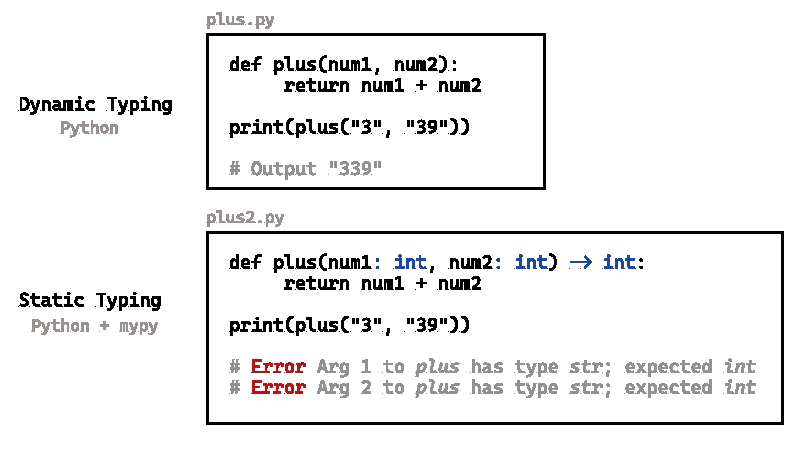
\includegraphics[width=\linewidth]{TypedVsUntyped.pdf}
  \caption[Comparison of the same program dynamically typed in Python and with mypy—a static typing tool for Python]{
    \label{fig:typed-vs-untyped}
    Comparison of the same program dynamically typed in Python (Top) and with mypy—a static typing tool for Python (Bottom).  The dynamic-typing rules of the Python interpreter apply, at run-time, the string concatenating version of the `+' operator -- regardless of the programmer's intention.  By contrast, mypy static-typing checks the type of the values passed to the {\tt plus} function against the intention declared by the programmer through the type annotations on the function parameters (both {\tt int}) and its return type (also {\tt int}).  The type check will fail until the programmer amends the function call with numeric arguments or otherwise explicitly converts the values from {\tt str} to {\tt int}.
    }
\end{figure}



\section{Functional Programming}

Alongside static typing, \textbf{functional programming} represents another rigorous approach to software development, drawing inspiration from Alonzo Church's lambda calculus in the 1930s \cite{Church1985-bx}. In functional programming languages, functions are the fundamental building blocks. They can be used as ordinary values, serving as both inputs and outputs for other functions, and can be combined to construct new functions. Programming in these languages centers around the composition of functions to perform high-level tasks. 
% Pure functional programming languages, characterized by immutable values and referential transparency, promote mathematical rigor. Immutable values ensure that once a value is declared, it cannot be altered. Referential transparency guarantees that functions will always produce the same output for identical inputs, providing predictable and testable code.

 A specific subset of functional programming languages, known as `pure' functional programming languages, incorporates additional mathematical rigor through concepts such as immutable values and referential transparency. Immutable values mean all values, once declared, cannot be modified. Referential transparency ensures that functions do not perform tasks that depend on external systems, such as reading from a global state, connecting to network resources, or even printing to the console.  These properties help mitigate undesirable programming behaviors similar to the way static typing does. For example, functional programming avoids issues like misaligned pointers and race conditions by disallowing mutable pointers and shared memory. Consequently, programs developed using these languages are more predictable and can be robustly tested and reasoned about \cite{Hu2015-ch}. This significantly reduces the risks that external factors could unpredictably affect program behavior, such as network fluctuations or even the passing of time \cite{Suzuki2019-bi}.

Functional programming is often advocated as an excellent choice for introductory programming courses due to its emphasis on mathematical reasoning and strict programming discipline \cite{Joosten1993-be, Chakravarty2004-ux}. This discipline includes the clear separation of data from its transformations, fostering a structured approach to problem-solving.


\begin{figure}[htbp]
  \centering
  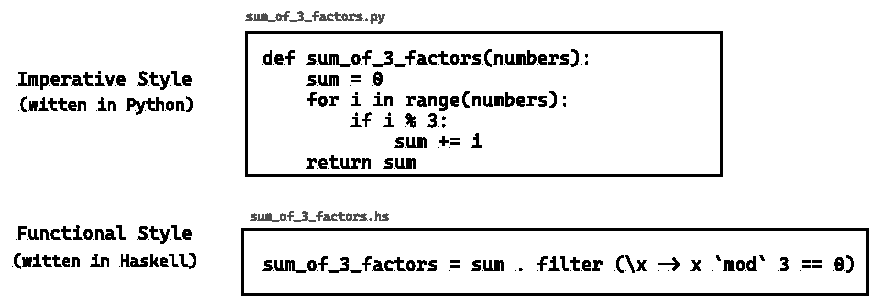
\includegraphics[width=\linewidth]{ImperativeFunctional}
  \caption[Comparing two approaches to implementing the same function specification in different programming paradigms: imperative and functional]{
    \label{fig:imperative-vs-functional}
    The figure compares two approaches to implementing the same function specification in different programming paradigms: imperative (top) and functional (bottom). The top section presents Python code, utilizing a loop and a mutable variable to accumulate sums. Conversely, the bottom section illustrates Haskell code, using a composition of two functions: \texttt{sum} and \texttt{filter}, the latter using a specified predicate in the form of an anonymous function. This exemplifies how imperative programming relies on mutable state (the \texttt{sum} variable) to track progress, whereas functional programming leverages high-level abstractions and recursion to achieve similar outcomes.    
    }
\end{figure}


Functional programming contrasts with other mainstream paradigms like object-oriented programming, which structures programs around objects combining data and behavior, and procedural programming, which focuses on a sequence of procedural steps. Despite the strengths of functional programming, object-oriented and procedural paradigms, exemplified by Java and C, respectively, remain more prevalent in commercial environments \cite{StackOverflow2023-cp, Cass2023-fa}. These paradigms benefit from extensive legacy codebases, broad third-party library support, robust tooling, and familiarity. Lastly, the rigor in functional programming languages may raise the barrier to entry for beginners. For example, in many pure functional languages, printing to the terminal window, generally considered a basic technique to observe the execution of the program, exposes programmers to profound concepts like monad and side effects, which can be daunting to those who are new to the language.  


\section{Statically-Typed Functional Languages, The Best Of Both Worlds}
Combining the disciplines described above, \textbf{statically-typed functional languages} employ both static typing and the principles of functional programming. The most common statically typed functional languages include Haskell,  ML (with the OCaml dialect being the most popular among the family of ML languages), and F\#. 
Of these, Haskell is the only ``pure'' functional language, with all variables being immutable by default.
Descendents of Haskell, like Idris and Agda, include more advanced type-level features like dependent type and session type, allowing programmers to express extremely granular checks of potential software behavior before running the program. These languages often provide the strongest level of programming safety. It is often advertised that programs in these languages will be error-free if the source code passes the compiling stage, indicating that compilers are able to weed out a large number of programming errors. These safety properties allow statically-typed functional languages to be used as proof assistants or formal verification tools. They prove the correctness (or incorrectness) of many systems, from web public key infrastructure \cite{Bhargavan2021-no} to microcontrollers used in space programs \cite{Mokhov2019-zj}. 

Despite these safety benefits, these languages' presence in the mainstream programming world remains underwhelming. This modest popularity is often attributed to high entry barriers, unfamiliarity with the paradigms, and advanced type systems that can be overwhelming for newcomers.

\section{Symptoms of Type Errors}
\label{sec:symptoms}
 The compiler is the medium through which programmers transform human intention into machine instructions. When encountering errors, compilers often act like Oracles in ancient history, revealing to programmers obscure messages that can lead to confusion and the wrong course of action. Many studies have investigated the ineffectiveness of compiler error messages \cite{Barik2017-gy, Becker2019-cs, Becker2016-kc}.  Our exploration is centered around type error messages (a subclass of compiler error messages) in the Haskell programming language and its leading compiler, Glasgow Haskell Compiler (GHC). It is vital to mention that the challenges discussed here concerning error messages are common across compilers for various statically typed languages. Below, we delve into specific issues often observed in type error messages.


 \subsection{Bias in Type Errors} 
 \label{subsec:bias}
 
A significant issue in type error messages is their inherent bias. Often, type errors can arise from multiple causes, but the error message might only highlight one. This issue is known as left-to-right bias in traditional type-checking algorithms—a notable shortcoming that limits the usability of error messages \cite{McAdam2002-vb, Lee1998-fx, Chen2014-ev}.  For instance, as shown in Figure \ref{fig:type-error-example}, a programmer likely intended to add two numbers using the \texttt{+} operator instead of mistakenly using the concatenation operator \texttt{++}. However, the type error reported by the compiler mistakenly points to the application of the integer literal \texttt{3}, failing to suggest the more probable cause. We will explore left-to-right bias further in Chapter \ref{chap:haskell-type-checking}.

 \begin{figure}[htbp]
  \centering
  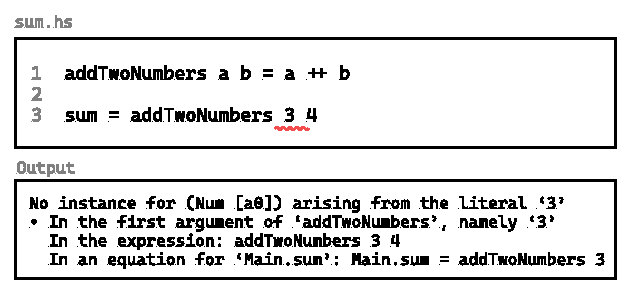
\includegraphics[width=\linewidth]{TypeErrorExample}
  \caption[Illustrating a programming error in Haskell, featuring a function named \texttt{addTwoNumbers} with a type error and the corresponding compiler output]{
    \label{fig:type-error-example}
    The figure illustrates a programming error scenario featuring the source code with a type error (Top) and the corresponding compiler output (Bottom). The error likely arises from the inappropriate use of the concatenation operator \texttt{++}, rather than the addition operator \texttt{+}, on line 1, as inferred from the function name \texttt{addTwoNumbers}. Despite this, the compiler erroneously highlights line 3, where the function \texttt{addTwoNumbers} is applied to the integer \texttt{3}, boldly assuming the correctness of the \texttt{addTwoNumbers} definition. This misdirection suggests a less likely source of error, potentially complicating the debugging process.
    }
\end{figure}


\subsection{Type Error Suggests Incomplete Cause}
\label{subsec:imcomplete}

Often, type error messages do not fully present all the locations relevant to the type error. Addressing the error at the recommended location might not suffice to resolve the underlying problem. Consider the scenario in Figure \ref{fig:type-error-example-2}, where a function intended for list concatenation is erroneously applied to integer values. Here, the error message only reports the first argument \texttt{3}, neglecting the second. This partial reporting leads to a situation where correcting the first argument to a list format, say \texttt{[3]}, doesn't rectify the error entirely; rather, it only updates to a slightly different error message. 



\begin{figure}[htbp]
    \centering
    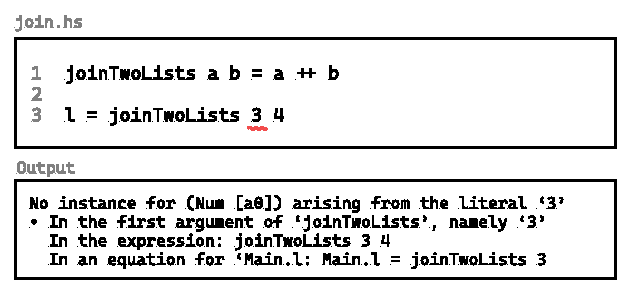
\includegraphics[width=\linewidth]{TypeErrorExample2}
  \caption[Illustrating a programming error in Haskell, featuring a function named \texttt{joinTwoLists} with a type error and the corresponding compiler output]{
    \label{fig:type-error-example-2}
    This figure depicts the same program as in Figure \ref{fig:type-error-example}, with one modification being the renaming of the function from \texttt{addTwoNumbers} to \texttt{joinTwoLists}. This change shifts the implied intent towards concatenating two \texttt{List} type values. The compiler still identifies an error at the same location—the integer literal \texttt{3}—aligning more closely with the programmer's understanding than in the previous example. However, the error message still misleadingly overlooks the erroneous type of the second argument, \texttt{4}, as it, too, is an invalid input for a list concatenation operation. Therefore, modifying only the first argument is insufficient to correct the type error.
    }
\end{figure}

\subsection{Missing Links In Type Errors}
\label{subsec:missing-link}

One of the most frustrating aspects of type errors is that they do not show the complete pathway of how the compiler decided on the type error. In the example in Fig \ref{fig:type-error-example-3}, the programmer may intend to compare to a char literal \texttt{' '} instead of string literal \texttt{" "} on line 1 in the function \texttt{isSpace}. However, multiple clues contribute to this conclusion. The definition of the function \texttt{trimWhiteSpace}, the application of \texttt{filter isSpace a}, the definition of \texttt{isSpace}, and even the type signature of \texttt{filter} all contribute to the logical reasoning. However, none of these are included in the actual error message.


\begin{figure}[htbp]
\centering  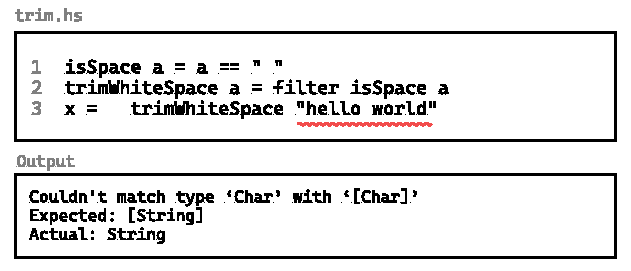
\includegraphics[width=\linewidth]{TypeErrorExample3}
  \caption[A type error in Haskell involving a type mismatch across multiple functions]{
    \label{fig:type-error-example-3}
    In Haskell, the \texttt{String} type is an alias for \texttt{[Char]}, meaning the two types are equivalent. The function \texttt{trimWhiteSpace}, as used on line 3, processes a \texttt{String} (or list of \texttt{Char} values) to filter out whitespace characters. However, the function’s filter condition, \texttt{isSpace}, erroneously compares two \texttt{String} values instead of \texttt{Char} types. This is likely a type intending the char literal \texttt{' '} rather than the string literal \texttt{" "}. While the type error message correctly identifies the mismatch, it fails to provide crucial contextual clues that would obscure the nature of this error.
    }
\end{figure}


\subsection{The Use of Obscure Language}

Error messages are frequently plagued by technical jargon and convoluted phrasing, which can be particularly off-putting for novices. An example is the error message, \texttt{No instance for (Num a) arising from the literal `3'}, which is an inept way of suggesting a type mismatch involving character and numeric types. In fact, this is often the common behavior across many programming languages and has been shown in many studies \cite{Barik2017-gy, Tirronen2015-nr, Prather2017-dg}. Thus, concerted efforts \cite{Becker2016-kc, Barik2014-ib}  show that rephrasing the error message to be clearer and more structured positively affects programmers' ability to solve these errors.


\section{The Challenges Of Making Good Type Errors}

After introducing some typical symptoms of bad type error messages, we will now explore some fundamental challenges to improve type error messages.

\subsection{Types Are Complex}

The advantages of statically typed languages derive from their robust type-checking systems, which, ironically, also introduce significant complexities. Language and tool designers frequently overlook the intrinsic complexity of type systems.  Type checking in these languages can exhibit Turing-complete characteristics, which might lead to non-terminating processes~\cite{Wells1999-ob}. TypeScript introduces `conditional types', a feature that allows sophisticated computations at the type level (Fig. \ref{fig:ts-conditional}), posing challenges in explaining errors when these type-level computations fail due to a lack of adequate debugging tools.



\begin{figure}[htbp]
  \centering
  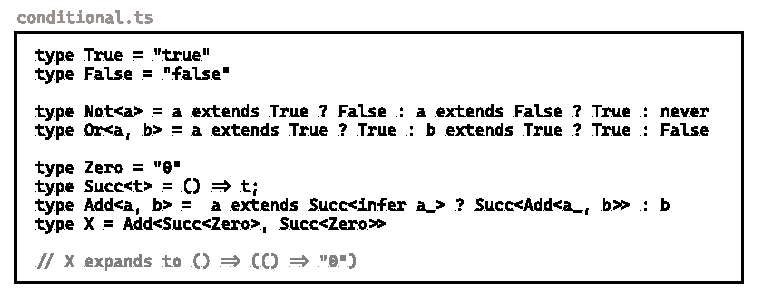
\includegraphics[width=\linewidth]{Conditional}
  \caption[An example of encoding propositional logic operators and church numerals in  TypeScript's conditional types]{
    \label{fig:ts-conditional}
    TypeScript includes a type-level feature known as `conditional types,' which enables the declaring of a type based on the outcome of a condition check. This capability is sufficient to construct a Turing-complete language within the TypeScript type system. The figure illustrates a simple language that supports booleans, numbers (using Church encoding), and functions that operate on these values. Since this implementation is implemented entirely at the type level, it does not generate any executable code for runtime evaluation, functioning purely within the compile-time environment. The recreational value aside, these type-level features often lead to elaborated ``essay of types'', hindering understanding and usability.
    }
\end{figure}

\subsection{Clues For Type Checking May Be Implicit}

The task of understanding how types are assigned in a program grows notably more complex when the programming language employs type inference. Type inference \cite{Damas1982-zw} is a technique that allows programmers to forgo the task of writing type annotations. Instead, the type checker automatically deduces the appropriate types for each expression based on the context. Although it succeeded in providing rigorous type checking without the hassle of manually writing type annotations, type inference has been shown to bring many usability issues \cite{Jun2002-xp, Wand1986-lu} for its implicitness.  

Even in programming languages that do not utilize implicit typing, certain typing rules remain opaque to programmers. For instance, rules on permissible values for equality check using the \texttt{==} operator vary across programming languages; some languages disallow comparison of lists, and others are fine with lists but disallow comparison of floating-point numbers. In languages that support a record data type, programmers must navigate additional complexities, such as whether adding or removing a field from a record maintains type correctness (Fig. \ref{fig:row-polymophism}). This often involves an understanding of nuanced language-specific rules, including concepts like covariance, contravariance, and subsumption.

\begin{figure}[htbp]
  \centering
  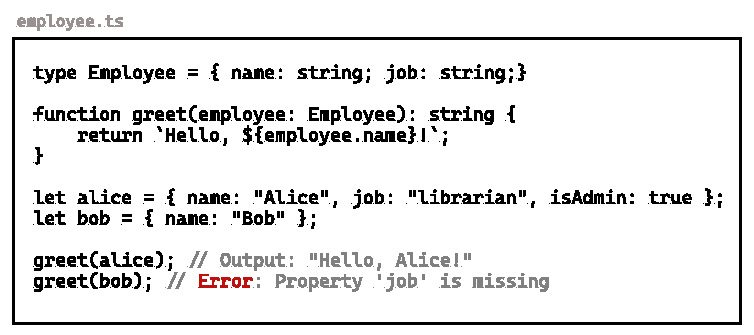
\includegraphics[width=\linewidth]{RowPolymorphism.pdf}
  \caption[An example of a correct usage and a wrong usage of row polymorphism in TypeScript]{
    \label{fig:row-polymophism}
Row polymorphism is a common type-level feature, allowing record values with optional more fields to be a subtype of the record without these fields. This enhances flexibility in structuring data collections but also introduces complexity in understanding the relations between types. The figure illustrates an example where programmers try to apply the record values \texttt{alice} and \texttt{bob} to the function \texttt{greet}. Because of the rules of row polymorphism and the fact that function arguments are covariant, only one value constitutes a valid input. 
    }
\end{figure}

These challenges amplify the difficulty in designing intuitive type error messages. The complexity of type systems demands that designers have a profound understanding of both theoretical and practical aspects of language implementation—knowledge often possessed only by the core language developers. Moreover, the implicit nature of modern programming languages requires that type errors be designed on a case-by-case basis, a daunting task given the limited number of contributors who possess the necessary expertise.

\section{The Lack of Type Debugging Tools}

Debugging programming errors have been an unpleasant but crucial part of programming since the inception of computing, tracing back to as early as 1949 \cite{Campbell-Kelly1992-rn}. However, the tools and support for debugging type errors have not evolved significantly and do not match the advancement of those available for runtime errors.

For runtime errors, one of the simplest and most effective debugging techniques is to insert \texttt{print} statements. As Brian W. Kernighan, one of the creators of the Unix system, once noted, ``The most effective debugging tool is careful thought, coupled with judiciously placed print statements'' \cite{Kernighan1978-xs}. Furthermore, breakpoint debugging has become a staple in nearly all programming Integrated Development Environments (IDEs), allowing for intermittent code execution and inspection (Fig. \ref{fig:breakpoint}). Research in error debugging tools continues to propose novel ideas. For instance, ZStep94 \cite{Lieberman1995-lg} enhances traditional breakpoint debugging by eliminating the need to set breakpoints, thus enabling programmers to view and navigate through the historical values that expressions take throughout execution (Figure \ref{fig:zstep94}). Another innovative tool, WhyLine \cite{Ko2009-uf}, aligns with the principles of a natural programming environment \cite{Myers2004-fy} by allowing programmers to ask ``why'' questions and ``why not'' questions about certain program behavior.

Despite these advancements in runtime debugging tools, the development of type debugging seems to have stagnated. Most programming languages and development environments still handle type errors in ways reminiscent of early languages like FORTRAN and ALGOL. In recent years, some modern programming languages like Elm and Rust have made efforts to improve type error reporting, but these enhancements are often superficial and do not fundamentally change the debugging experience \cite{Ferdowsi2023-au}.


\begin{figure}[ht]
  \centering
  \includegraphics[width=\linewidth]{BreakPoint}
  \caption[Debugging of a Python program using a breakpoint and expression evaluation in PyCharm]{
    \label{fig:breakpoint}
    The figure shows the debugging of a Python program using a breakpoint and expression evaluation in PyCharm, a widely used interactive programming environment (IDE) for Python. Program execution is paused at the breakpoint set on line 4, and with each pause, the user-defined expression \texttt{i * j} is re-evaluated. This common debugging interface is available in nearly all modern programming editors and integrated development environments.
    }
\end{figure}


\begin{figure}[ht]
  \centering
  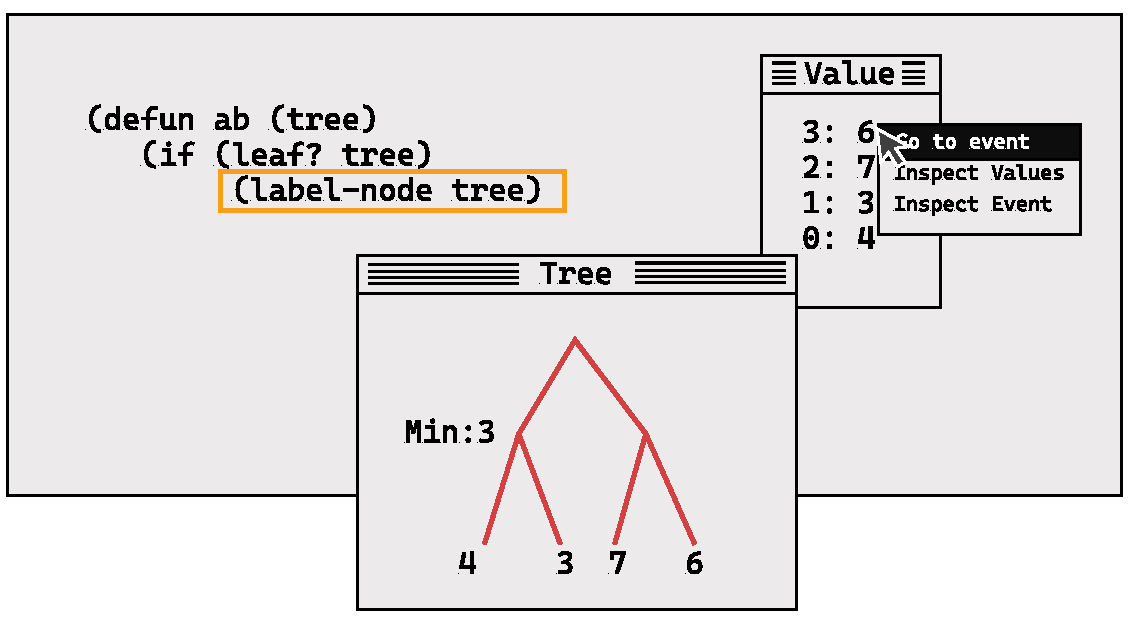
\includegraphics[width=\linewidth]{ZStep94}
  \caption[Debugging a Lisp program by inspecting all the historical values of an expression in ZStep94]{
    \label{fig:zstep94}
    Debugging a Lisp program by inspecting all the historical values of an expression, navigating through execution history, and reviewing live visualization replay.  All these features are provided in ZStep94.
    }
\end{figure}

My research is driven by the acknowledged difficulties in debugging type errors and the lack of significant advancement in the interfaces and techniques used for presenting and resolving these errors. This area holds considerable potential for improving both the usability and accessibility of statically typed languages, making them more approachable for developers at all levels of expertise.

\section{Research Aim}

\subsection{Aim 1. Provide programmers with the comprehensive knowledge needed to understand and resolve type errors.}
\label{subsec:aim1}

Current representations of type errors in most compiler tools are often insufficient for straightforward resolution without further investigation by the programmer. They typically provide only the location of the type check failure, the expected type, and the actual type encountered. This conventional approach, as discussed in the previous sections (\ref{sec:symptoms}), lacks practicality and clarity. This aim addresses the need for a richer, more informative explanation of type errors by evaluating the limitations of existing systems and analyzing how programmers tackle type errors in practice.

\subsubsection{Objective 1.1 To Encompass Multiple Potential Causes Of A Type Error}
An essential aspect of this research is to challenge and expand beyond the bias found in traditional type error reporting (Section \ref{subsec:bias}). It's crucial to inform programmers that multiple potential causes and resolutions are almost certain to be present in every type error. A key goal is to communicate the dimension of multiple potential causes effectively. In addition, for each potential cause, programmers need a clear explanation of where the offending code is, which typing rules are violated, and most importantly, how the meaning of the program will change after the error is resolved.


\subsubsection{Objective 1.2 To Accurately Report Relevant Locations Contributing to Type Errors.}
Current tools often pinpoint a single location for a type error, a method that has attracted considerable criticism for its inefficiency. Programmers frequently need to scan beyond the initially reported location. This research aims to enhance type error reporting by identifying and detailing all relevant error-contributing locations across the codebase.

\subsubsection{Objective 1.3 To Give Reasons And Support Human Understanding}
Understanding type errors goes beyond pinpointing the location in the code. Internally, type errors can be caused by mismatched types, unmatched type class constraints, and trying to construct infinite types, among other reasons. Externally, type errors can be caused by typos, outdated type annotation, incomplete implementation, etc. Our goal is not only to locate these errors but to explain them in a way that logically supports the programmer's understanding and troubleshooting process, covering both internal causes and external causes.



\subsection{Aim 2. Support Programmers To Type Errors Through Interactive Modern Programming Environments.}

This aim focuses on integrating comprehensive type error encoding (Section \ref{subsec:aim1}) within an interactive programming environment to streamline workflows in statically typed languages. Although aim 1 focuses on enriching the information of type error,  we acknowledge that an increase in information does not necessarily correlate with enhanced understanding. Thus, this aim also focuses on presenting the details of type errors intelligently to optimally support comprehension and resolution.

\subsubsection{Objective 2.1 Visualize The Key Concepts Of Type Errors Effectively}

Traditional text-based error reports can be difficult to navigate and understand. This objective explores innovative methods to present what used to be displayed as plain text (type signatures, locations in source code, call stacks, dependency graphs) in graphic user interfaces. Examples include in-line highlighting within the code editor and graph-based reasoning steps.  

\subsubsection{Objective 2.2 Use Interactive Tools for Investigating and Resolving Type Errors.}

This objective focuses on using interactive techniques to improve the usability of type errors.  This includes using interface elements that allowing user input (hover, click, drag and drop, etc) to trigger common debugging tasks. In addition, this objective also encompasses providing context-sensitive debugging aids that adjust the interactive response based on the current performing task, error type, and individual user preferences.


\section{Contributions}

\subsection{A categorization of type errors based on the structure of the evidence of a type error}

To address the complexities in explaining type errors comprehensively, we have classified type errors into three categories based on how human programmers perceive type errors. Formal definitions and a detailed discussion of these categories appear in Chapter \ref{chap:haskell-type-checking}. It is crucial to understand that these categories are not mutually exclusive; for example, a multi-witness type error may also be a multi-step type error.

A \textbf{multi-step type error} involves a chain of logical inferences steps based on the available evidence of the error. Figure \ref{fig:multi-step-example}) illustrates the chains of inference in the assignment of a (Line 1), the equivalence of a (Line 1 and Line 2), the assignment of b (Line 2), and the equivalence of b (Line 2 and Line 3). Removing anyone from the chains will resolve the conflict. Understanding and communicating the interconnections within these chains is crucial to resolving multi-step type errors effectively.

\begin{figure}[htbp]
  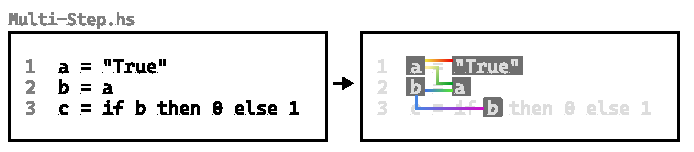
\includegraphics[width=\linewidth]{Multi-Step}
  \caption[This illustration depicts a multi-step type error in Haskell]{
    \label{fig:multi-step-example}
    This illustration depicts a multi-step type error in Haskell. In the program (left panel), the string literal \texttt{"True"} is assigned to the variable \texttt{a} on line 1, followed by the assignment of \texttt{a}'s value to variable \texttt{b} on line 2. Subsequently, on line 3, the program attempts to use \texttt{b} as a boolean condition in an \texttt{if} expression. The error analysis can be visualized as a "chain" of reasoning, represented by the continuous line (right panel), tracing the propagation of the type mismatch through the sequence of assignments and usage. }
\end{figure}

A \textbf{multi-witness type error} involves multiple pieces of evidence supporting the same potential type assignments. For instance, as shown in Figure \ref{fig:multi-witness-example}, multiple evidence (lines 3,4,5) support that \texttt{a} has the type \texttt{Int -> String}. On the other hand, a single piece of evidence (line 2) shows that \texttt{a} has the type \texttt{Int -> Char}.  Clarifying and juxtaposing this discrepancy in witnesses is key to supporting understanding this type of error.

\begin{figure}[htbp]
\centering  \includegraphics[width=\linewidth]{Multi-Witness}
  \caption[This illustration depicts a multi-witness type error in Haskell]{
    \label{fig:multi-witness-example}
    This figure presents the analysis of a multi-witness type error in Haskell. In the source code (Left), a type conflict arises from the \texttt{case} expression, which could be interpreted as \texttt{Char} based on the value in line 2, or as a \texttt{String} based on the values in lines 3, 4, and 5. The type conflict is graphically illustrated (Right) with \texttt{String} values marked in pink and the \texttt{Char} value in blue. The majority of \texttt{String} value witnesses suggest the lone \texttt{Char} literal \texttt{'I'} on line 2 might be a typographical error. This discrepancy underscores the significance of witness count in identifying the likely error source.}
\end{figure}

A \textbf{multi-party type error} involves several potential type assignments, each supported by distinct evidence.  Figure \ref{fig:multi-party-example} presents a typical multi-step type error: the expression \texttt{d} can not be assigned a type because 3 pieces of evidence on line 1 suggest 3 potential types for \texttt{d}. In practice, addressing such errors requires breaking them down into multiple type errors of simpler forms.


\begin{figure}[htbp]
\centering  \includegraphics[width=\linewidth]{Multi-Party}
  \caption[This illustration depicts a multi-party type error in Haskell]{
    \label{fig:multi-party-example}
    This figure analyzes a multi-party type error in the source code (Left), where the list \texttt{d} could potentially be typed as \texttt{[Int]}, \texttt{[String]}, or \texttt{[Char]}. The disagreement is visually represented (Right) by three distinct colors, each corresponding to the cause of one of the possible types. This scenario differs from previous examples as resolving the type error requires adjustments at multiple locations within the code, not just a single change.
       }
\end{figure}

These classifications have led to the development of three distinct systems—\chameleon{}, Goanna, and GeckoGraph—each designed to tackle unique challenges within the domain of type error debugging.

\subsection{Explain Multi-Step Type Errors Through Chain-Of-Thought Visualization}

\subsubsection{Technical Contribution - \chameleon{}}


We contribute \chameleon{}, an interactive Haskell debugging tool that identifies all relevant error-contributing locations and illustrates the logical relationships between these locations. 


Our contribution in \chameleon{} benefits from the existing work on Chameleon \cite{Stuckey2003-pz, Wazny2006-ll}. Originally,  Chameleon was developed as a command-line tool. Its novel ideal of interactive debugging allows programmers to view different possible type error explanations and type assignments by issuing console commands. Besides, Chameleon successfully encoded the Haskell type system, with the addition of functional dependency, entirely in constraint handling rules \cite{Fruhwirth1998-jq}. \chameleon{} shares the theoretical foundation with the original Chameleon, providing a modern implementation with many advanced features. Notably, \chameleon{} provides a novel debugging interface to interactively explore the chain of reasoning in a multiple-step type error, allowing programmers to interactively develop a panorama view of the type error. In addition, \chameleon{} uses an adaptive interface design; programmers can switch between different granularity of information based on their personal preferences. 


\subsubsection{How programmers use type error slicing and chain of thought visualization to understand type errors}

We conducted a series of three user studies to investigate the effect of type error slicing and interactive type error exploration. We compared how programmers solve type errors with \chameleon{} and with traditional compiler tools. Our findings show a notable improvement in debugging speed when using type error-slicing, particularly for complex tasks. Additionally, we observed a significant enhancement in debugging speed when programmers actively use the interactive debugging features, suggesting that interactive exploration of type errors can positively impact the debugging process.

\subsection{Resolve multi-witness and multi-party errors with Minimal Correction Subsets}
\subsubsection{Technical Contribution -- Goanna}
We provide Goanna, a Haskell type error debugging tool. Goanna enhances type error debugging in Haskell by identifying all relevant error-contributing locations and presenting all possible causes and their respective resolutions. It ranks the potential causes of type errors based on their likelihood, helping programmers identify the root causes with minimal interactions with the tool.

\subsubsection{An evaluation of the effectiveness of MCS-based type debugging tools}


To evaluate the effectiveness of the MCS-based type error debugging approach, we compiled a dataset of 86 Haskell programs from various online discussion platforms, covering a broad spectrum of type error themes. We tested the accuracy of Goanna in identifying and resolving type errors, comparing it to traditional compiler tools. Our research confirms that Goanna consistently outperforms other tools in pinpointing the correct cause of errors. Moreover, Goanna's heuristics effectively narrow down potential causes and consistently include the real cause among its top suggestions. Although Goanna operates moderately slower than standard tools, its processing time remains sufficiently quick to offer real-time feedback to developers. 

\subsection{Visualizing Types}

\subsubsection{Technical Contribution -- GeckoGraph}

We contribute GeckoGraph, a graphic notation for Haskell types. GeckoGraph encodes the same information as type signatures but uses colors, shapes, and symbols to make certain structures easy to identify at a glance. GeckoGraph uses visual elements to improve the understanding of complex type concepts, such as type classes and qualified constraints. GeckoGraph offers clarity when reading complex type signatures and comparing multiple types.

\subsubsection{An evaluation on how programmers use diagrammatic type notation}

We conducted a large-scale user study to assess the effectiveness of GeckoGraph in improving upon the traditional text-based approach to type signatures. The user study was designed as an interactive puzzle game with gamification elements to boost participation and engagement. A total of 721 programmers, ranging in experience levels, took part in the study. The findings indicated that while GeckoGraph did not enhance the speed or overall success rate of problem-solving significantly, it was notably beneficial in aiding beginners with more challenging tasks. Feedback gathered through a qualitative post-study survey was positively inclined, highlighting that GeckoGraph is intuitive, non-intrusive, and helpful.

% \section{Research Method}

% \subsection{Human-centered programming language studies}

% One important decision that shape a lot of my work is employing human-centered research methods with our novel programming language systems. The adopting of human-centered methods happens at every stage of the projects: prototyping, development and evaluation. Although the using of these methods are not new at all, but they certainly are not the most polular choices in programming language studies.

% The motive of such decision is that it is impossible to understand what are the good qualities of type errors without observing how human use type errors to gain understanding. 


% The downside of study programming language is iterative design is very hard. programming tasks involves complex inputs and outputs, and it is very hard to study an incomplete system without a fully working systems. For instance, if we are to study the effect of type errors, it is most effective to have a system that can recognize type-correct program from ill-typed one. It is hard to evaluate with a mock-up or wizard of oz style fake outputs to study users' interaction.  To address this limitations, we have a few ideas implemented in our research:

% A minimal but practical set of language 
% Design for human from start



\section{Thesis outline}

 This thesis is structured into two main parts. The initial chapters (Chapters \ref{chap:introduction}, \ref{chap:haskell-type-checking}) build a comprehensive foundation on type systems and programming languages, setting the stage for my research contribution in subsequent chapters. The latter chapters focus on distinct contributions that tackle various challenges in type error debugging.

\subsection{Chapter 1: Introduction}
Chapter 1 sets the stage by discussing the fundamental concepts of programming languages and type systems. It explores the trade-off between enhancing program safety and optimizing usability, a central dilemma in programming language research and software engineering practice. The chapter highlights common issues and technical challenges associated with type errors, establishing the motivation for this research. It also outlines the specific aims and contributions of the study, providing a roadmap for the thesis.

\subsection{Chapter 2: Haskell Type Checking}
This chapter delves into the fundamental concepts underlying type systems and programming languages. It outlines traditional methods employed in Haskell type checking, error slicing, and interactive debugging. Additionally, this chapter discusses tools and techniques used in constraint satisfiability analysis that are integral to later developments in the thesis. The categorization of type errors is revisited and redefined, building on the definitions introduced in this chapter.
    
\subsection{Chapter 3: \chameleon{} -- Interactive Type Error Visualization and Exploration}
Chapter 3 presents \chameleon{}, a system designed to enhance the debugging of type errors through interactive visualizations. It begins with a discussion on the typical pitfalls of existing error messages and outlines the motivation behind \chameleon{}. We then detail the system's design, features, and development process, including iterative prototyping. A series of empirical studies were conducted to assess \chameleon{}'s effectiveness compared to traditional compiler tools.
    
\subsection{Chapter 4: Goanna -- Finding All Type Errors Using Minimal Correction Subsets}
Chapter 4 introduces Goanna, a Haskell type error debugging tool that incorporates novel features such as suggesting fixes for type errors and cross-module debugging capabilities. It starts with highlighting the limitations of conventional compiler error messages and progresses to describe Goanna's capabilities in identifying all causes and ranking potential causes by their likelihood. The implementation tactics and heuristic methods used in Goanna are discussed, followed by an empirical evaluation of the system's accuracy, conciseness, and performance based on real-world Haskell code examples.
    
\subsection{Chapter 5: GeckoGraph — A Graphic Notation For Haskell Types}
Chapter 5 introduces our design of GeckoGraph. GechoGraph is a graphic notation for Haskell types. This chapter starts by underscoring the challenges of understanding and using polymorphic types. It then introduces GeckoGraph, how it addresses these challenges, and how to constructively transform text-based type signatures to GeckoGraph. We then showed our experiment on evaluating the effect of using GeckoGraph to help solve program tasks. Lastly, we discussed the strengths, limitations, and potential applications of GeckoGraph and type visualizations in general.   
    
\subsection{Chapter 6: Conclusion}
The final chapter reiterates the thesis's contributions. It discusses potential avenues for future tool development and research opportunities, forecasting the future landscape of programming language research. The chapter concludes with reflections on the importance of improving type error diagnositics, encouraging ongoing investigation and innovation.
% 

% Chapter 2

\chapter{Background}

Programming in strongly typed languages has many advantages. It helps programmers identify logical errors before running the code, reduce maintenance difficulty, and improve the editor capability find documents and auto-complete code while typing. However, the difficulties in understanding and resolving type errors often ward people off  from practicing strongly typing.  In this Chapter, we discuss the relevant research in improving the experience of debugging type errors. We first investigate the theoretical approaches to enrich/correct the information presented type errors. We then  investigate the various designs of tools, interfaces, and visualizations to support understanding type errors.

\label{chapter2} 




\section{Challenges in Debugging Type Errors}

\subsection{Left-right bias}

\subsection{Reporting Non-leaf nodes}

\subsection{Remembering intermediate steps}

\subsection{Polymorphic Types}

\section{Approaches to Support Debugging Type Errors}

\subsection{Type error slicing}

\subsection{Search based debugging tools}

\subsection{Error tolerant tools}

\section{Interactive Debugging Tools}


% Chapter Template

\chapter{Haskell Type Checking} % Main chapter title

\label{chap:haskell-type-checking}

\graphicspath{{Figures/HaskellTypeChecking}}

In Chapter \ref{chap:introduction}, we briefly explored the history of programming languages with an emphasis on their practices in type checking and the paradigms they employ. This chapter focuses exclusively on Haskell, outlining why it is particularly well-suited for studying improvements in type error detection. We delve into the common techniques for performing type-checking on Haskell programs, specifically the Hindley-Milner type inference system and Algorithm W.

Furthermore, we examine various approaches that have been explored to provide better error messages, including Algorithm M, type error slicing, and interactive debugging. We also discuss key developments in the realm of constraint satisfiability, highlighting their significance to enhancing type error messages. Finally, we revisit the categorization of type errors, this time in light of the aforementioned techniques and tools.

\section{Why Haskell}

Haskell, introduced in 1990, is a functional programming language renowned for its enforcement of pure functional principles, lazy evaluation, and an expressive type system. The primary focus of my work is to develop type debugging systems for Haskell that leverage this expressive type system and address its limitations. Although we plan to extend our work to other languages, there are compelling reasons for initially focusing on Haskell.

\subsection{Haskell In Education}
As discussed in Chapter \ref{chap:introduction}, Haskell plays a significant role in undergraduate computer science education and was designed with this educational purpose in mind. Many textbooks targeting first-year computer science courses and introductions to functional programming recommend Haskell as a pedagogical tool \cite{Bird1998-kv, Davie1992-xv}. Proponents argue that Haskell serves as an ideal platform for teaching programming and rigorous reasoning due to its mathematical nature. Students often find that Haskell "elegantly admits solutions that are difficult to formulate in imperative languages," a sentiment echoed by computer scientist Edsger W. Dijkstra in a letter advocating for the use of Haskell for freshmen at the University of Texas, instead of Java.

Despite Dijkstra's enthusiasm, actual adoption in universities has been modest. One frequent challenge in teaching Haskell is helping students overcome programming errors \cite{Jun2000-yu, Tirronen2015-nr}. Some recommend using a simplified subset of Haskell's features to avoid the frustrations associated with complex type errors \cite{Heeren2003-mz}. Our research is motivated by both the desire to enhance Haskell's educational value and the real-world challenges associated with teaching the language.

\subsection{Haskell's special position in programming language research}

Although the full semantics of Haskell have never been formally defined \cite{Hudak2007-kn}, this has not deterred its use as a platform for programming language innovation or for meaningful academic contributions. Subsets of Haskell can be formalized for rigorous language study \cite{FaxEn2002-nd}. Haskell's dual presence in academia and the mainstream programming world uniquely positions it as a testing ground for new programming language features and ideas. Indeed, features such as Haskell's list comprehension have been adopted by languages like Python and Julia, and its generic type systems have influenced languages such as Java, C\#, and Rust.

Our research in Haskell benefits from the language's relatively small and well-studied specification, enabling rapid implementation of new ideas and swift feedback. We also enjoy support from Haskell's welcoming and active community, which helps guide our efforts towards improved correctness and usability.

\section{Hindley-Milner Type Inference and Algorithm W}

Type inference, also known as implicit typing, is a technique to reduce the number of occurrences of manually ascribing types. Almost all languages today employ a certain level of type inference. For instance, Java versions prior to 10 required users to explicitly declare variable types, which often led to verbosity and redundancy, as shown in Figure \ref{fig:example-java}. Java later introduced the var keyword (from version 10 onwards), allowing the type of a variable to be inferred at compile-time based on the assigned value \cite{noauthor_undated-an}.  

\begin{figure}[hbt]
  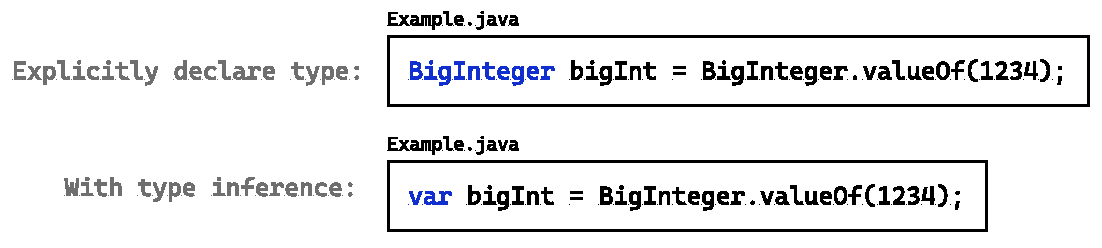
\includegraphics[width=\linewidth]{ExampleJava}
  \caption{
    \label{fig:example-java}
      An example of a typical Java program before and after introducing the \texttt{var} keyword. Before (Top), programmers have to annotate the type identical to the value initializer. After Java 10, this is solved using the local type inference with the \texttt{var} keyword (Bottom).
    }
\end{figure}

In language like Haskell and ML, not only is type inference applied, but its power to detect type error is hugely amplified by the use of the Hindley-Milner type inference  \cite{Damas1982-zw}. The Hindley-Milner Type System  named after its inventors Roger Hindley and Robin Milner, is a type system that can automatically infer the types of expressions in a language with no annotations required. It is a foundational part of the type system in many functional programming languages, including ML, Haskell, and Elm. The system provides polymorphic typing, meaning that a variable can be assigned multiple different types automatically based on its usage context, making it easier to write flexible, reusable code without compromising type safety. In many languages that use this system, it is proven that every expression will be assigned a most general type (principal type) based on its usage. 


In simpler type inference systems, such as the one used in the Java example (Fig \ref{fig:example-java}), type inference is local; it occurs within individual assignments and the compiler may raise errors if it cannot infer types from a single statement. In contrast, the Hindley-Milner system  employs a more global approach. It defers type constraints resolution and continues to assess the rest of the program, thereby increasing flexibility and reducing the immediateness of type errors.




\begin{figure}[hbt]
    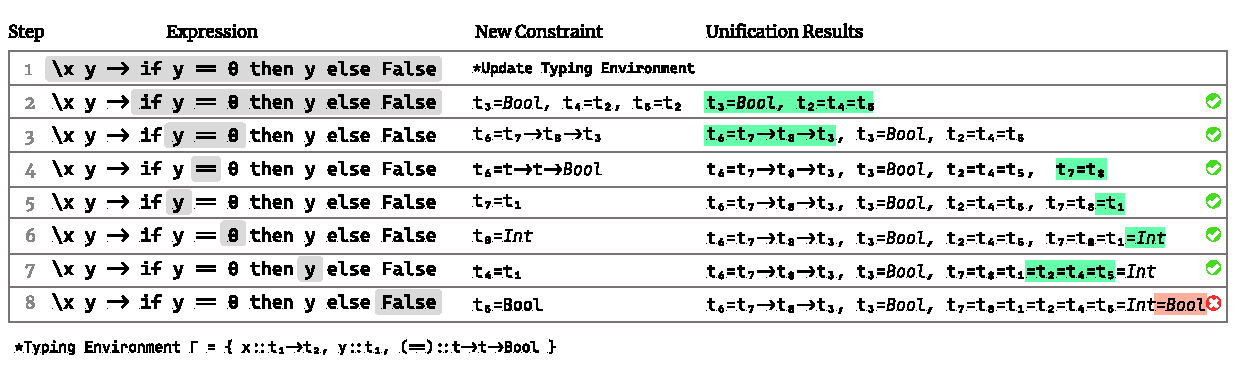
\includegraphics[width=\linewidth]{HindleyMilner}
    \caption{
      \label{fig:hindley-milner}
        An illustration of Hindley Milner Type Checking Performed on a Lambda Expression, \todo{Expand this figure}}
\end{figure}

This sophisticated type inference mechanism found in the Hindley-Milner system underpins its wide adoption in the realm of functional programming. It exemplifies a shift towards more intelligent compilers that enhance developer productivity and code maintainability by abstracting the complexities of explicit type management.

\textbf{Algorithm W}  The foundational mechanism of the Hindley-Milner type system is Algorithm W, a method designed to deduce the most general types for each expression in a program. This algorithm starts by assigning a unique type variable to each expression. It then recursively analyzes the structure of the program, generating a set of type constraints by inspecting each syntax node—as shown in Figure \ref{fig:hindley-milner}. This process involves the creation of new type variables and the unification of these variables with others or with specific types.

Unification is a critical step: it attempts to make different type variables agree by finding a common type that satisfies all constraints. If unification is unsuccessful at any point, the type checking process halts immediately, indicating a type error. The algorithm report the expression where the last constraint was produced, but this is often reported as the sole source of the error.


Despite the seismic influence in type theory, and the conciseness of programming style it helps achieved,  the Hindley-Milner type system can be challenging in terms of usability. One notable drawback is how it handles error reporting. When type inference fails, the error messages can be cryptic and difficult to interpret. This is because the algorithm typically reports only the final constraint that led to the failure, omitting earlier but potentially relevant constraints. Unlike simpler cases in languages like Java—where a type error might be isolated to a single line—in a Hindley-Milner-based system, the underlying issue could be located anywhere in the program. This often leaves programmers scanning extensive sections of code to identify the root cause of the error. 

This aspect of Algorithm W highlights a trade-off between the power of the type inference offered by the Hindley-Milner system and usability, notably in terms of error diagnostics and clarity. This has prompted ongoing research into improving error reporting in systems based on this algorithm, seeking to make them more accessible and easier to use for programmers.

\textbf{Algorithm M} 
In response to the usability challenges posed by Algorithm W, an alternative approach known as Algorithm M was proposed \cite{Lee1998-fx}. This method modifies the direction of type inference from a bottom-up to a top-down process. By carrying constraints from the outer structure of the program to the substructures, Algorithm M allows for a more contextual analysis, resulting in more intuitive error messages in certain scenarios, as illustrated in Figure \ref{fig:algorithm-m-1}. 

\begin{figure}[hbt]
  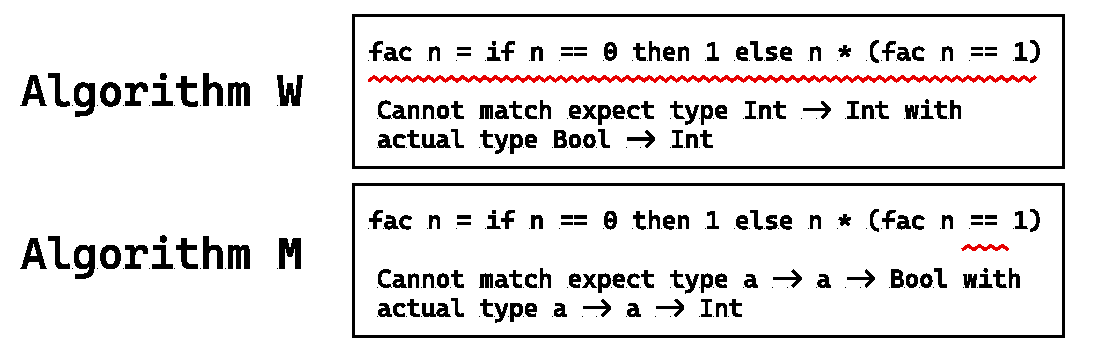
\includegraphics[width=0.8\linewidth]{AlgorithmWM1.pdf}
  \caption{
    \label{fig:algorithm-m-1}
      An example where Algorithm M out-guessed Algorithm W, reporting a more plausible error location.}
\end{figure}


\begin{figure}[hbt]
  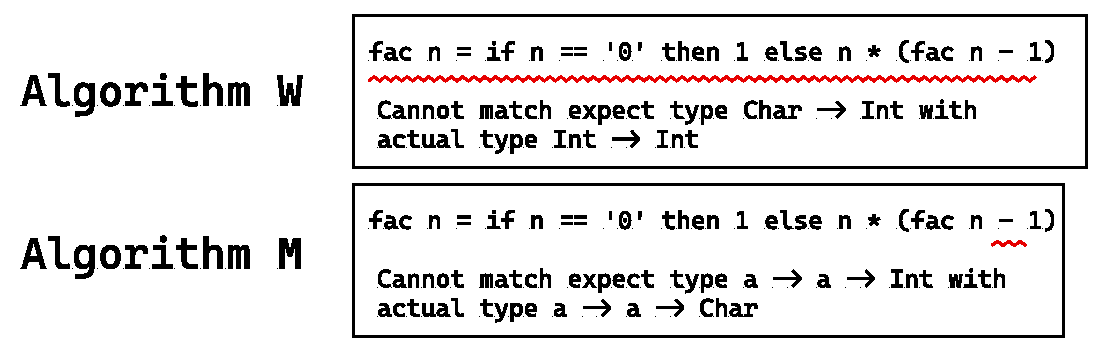
\includegraphics[width=0.8\linewidth]{AlgorithmWM2}
  \caption{
    \label{fig:algorithm-m-2}
    An example where Algorithm M may miss the correct location. It is more plausible here that \texttt{'0'} is a typo.}
\end{figure}


Despite its improvements in some cases, Algorithm M does not consistently outperform Algorithm W in terms of error clarity and can still produce misleading results, as shown in Figure \ref{fig:algorithm-m-2}. Both algorithms essentially face the same fundamental limitation: type inference is conducted step-by-step through unification, and once constraints are unified, they are discarded an unretrivable. Consequently, errors detected by these algorithms may not accurately reflect the root issues if multiple possible causes of types exist.

A lesson can be learned learned from both Algorithm W and M is the recognition that no inference method ensure that it will perfectly align with the programmer’s intentions. Rather than ambitiously pinpointing where the root cause may lie, a more realistic goal might be to represent type errors succinctly without making assumptions.


\section{Type Error Slicing}

Type error slicing is an advanced technique intended to enhance the meaningfulness of type error messages provided to programmers. This approach, referenced in works by Tip \cite{Tip2001-qn} and Haack \cite{Haack2004-fr}, improves upon traditional type inference methods by postponing the unification process until all relevant constraints have been established. Type error slicing incorporates two principal innovations:


\begin{enumerate}
  \item {
    \textbf{Labeled Constraints:}
    This involves assigning identifiable labels to constraints based on their locations within the program. These labels are subsequently used to trace and diagnose parts of the code associated with a type error, offering clearer insights into the origins of an error.
  }
  \item {
    \textbf{Minimal unsatisfiability analysis:} 
    This technique focuses on identifying the smallest set of conflicting constraints that cannot be satisfied simultaneously. This means finding the necessary evidence needed to reproduce the failed unification but nothing more than that. This approach significantly improve the diagnosis of type errors by avoiding the biases found in both Algorithms W and M.
  }
\end{enumerate}


\begin{figure}[hbt]
  \includegraphics[width=0.5\linewidth]{TypeErrorSlicing.pdf}
  \caption{
    \label{fig:type-error-slicing}
      An example of type error slicing}
\end{figure}

In contrast to conventional methods, type error slicing provides a comprehensive view of error locations, as demonstrated in Figure \ref{fig:type-error-slicing}. It allows programmers to understand type errors more thoroughly by presenting both sides of typing conflicts, thus facilitating a more informed debugging process.

Over time, type error slicing has become a preferred method for optimizing type errors. Innovations in this area include more efficient methods of finding minimal unsatisfiable subsets \cite{Liffiton2008-mx, Bailey2005-hi, Bacchus2015-of}. Type error slicing has also been enriched by exploring various underlying constraint languages that encode more complex type system features, such as those using SMT (Satisfiability Modulo Theories) \cite{Pavlinovic2015-ke} and Constraint Handling Rules \cite{Stuckey2003-pz}. These advancements have broadened the scope and applicability of type error slicing, making it a valuable tool for programming language development and error diagnosis.


\section{Interactive Type Debugging}

Traditional error diagnostic methods, such as the Minimal Unsatisfiable Subset (MUS) approach, have been instrumental in localizing single type errors by pinpointing a comprehensive yet minimal set of related code locations. Despite their utility, there are several key limitations associated with MUS-based localization and diagnosis:

\begin{figure}[hbt]
  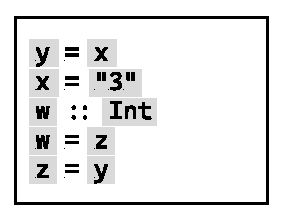
\includegraphics[width=0.5\linewidth]{SlicingCounterExample}
  \caption{
    \label{fig:slicing-counter-example}
      An example where type error slicing essentially highlights every location in the program.}
\end{figure}

\begin{enumerate}
  \item {
    \textbf{Limited Code Reduction:} Although MUS-based error slicing can effectively narrow down the potentially defective code areas, studies such as Binkley's empirical analysis on program slicing \cite{binkley_empirical_2007} suggest that this method only reduces about 30\% of the code that needs to be examined to understand a type error. The minimal nature of MUS often prevents further reduction, which can be insufficient for complex errors as demonstrated in Figure \ref{fig:slicing-counter-example}, where virtually every location in the program could be implicated in the error.
  }

  \item{
    \textbf{Lack Of Enhanced Information Encoding:}  The existing MUS-based approaches might highlight critical error sites, but they often fail to capture the breadth of information required to fully understand and resolve type errors, especially in systems with complex type features.
  }
\end{enumerate}

To address these limitations, pioneering tools like Chameleon \cite{Stuckey2003-pz} have been developed. Initially introduced in the early 2000s, Chameleon served as a command-line tool aimed at improving type error reporting within the Haskell programming language. Unlike typical type-error slicing methods, Chameleon utilizes a more expressive constraint language—Constraint Handling Rules (CHR)—which enables the support of more flexible relational constraints tailored to advanced type-level features such as type classes and functional dependencies.

A key innovation of Chameleon is its adoption of interactive type debugging. This approach not only identifies potential error locations but also reveals that there could be multiple sets of potential types—most general unifiers—that could resolve the type issues present in the defected program. These types are traceable to distinct sets of code locations.

With interactive type debugging, programmers can query the type information of any possible resolution, effectively allowing programmers to ask counterfactual questions such as ``what would the type of the expression be if the type error is fixed". This interactive process significantly advances the programmers' understanding of type errors by allowing them to explore different resolution paths and better comprehend the type system's behaviors and expectations.

Interactive type debugging thus represents a significant evolution in the handling of type errors, offering a more dynamic and informative approach compared to static slicing methods. This development underscores a shift towards more user-centered diagnostics tools in programming, where clarity and interactivity play vital roles in problem-solving.

\begin{figure}[hbt]
  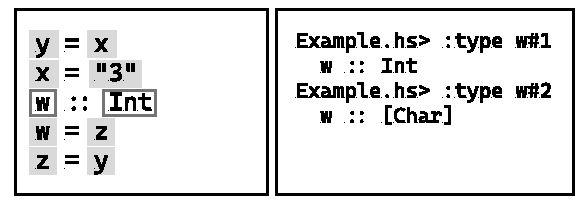
\includegraphics[width=0.8\linewidth]{ChameleonInteractive}
  \caption{
    \label{fig:chameleon-interactive}
      An example where type error slicing essentially highlights every location in the program.}
\end{figure}

\section{The Analysis Of An Unsatisfiable System}

One advantage of using a slicing-based approach is that many tools are available from the study of constraint satisfiability. Among them, a few important ones are the Minimal Unsatisfiable Subset (MUS), Minimal Correction Subset (MCS), and Maximal Satisfied Subset (MSS).  

\subsection{Minimal Unsatisfiable Subset}

MUS is the most commonly used tool in programming error analysis. Most program slicing-based tools \cite{Haack2004-fr, Pavlinovic2015-ke, Stuckey2003-pz} use MUS one way or another. Intuitively, MUS is the smallest subset of a constraints system that still remains infeasible. Infeasibility here simply means there are no ways to assign value to the logical variables. For an ill-typed program, this means finding a minimal set of locations that can explain the logical conflict of a type error. 

Formally,  a minimal unsatisfiable subset (MUS) $M$ of a constraint system $C$ is a subset $M \subseteq C$ such that $M$ is unsatisfiable and $ \forall{c} \in M : M \setminus \{c\}$ is satisfiable. An MUS can be seen as a minimal explanation of the infeasibility of the constraint system. MUSes have been used extensively, mostly in combination with programming slicing, as a means to explain type errors. A MUS of type system constraints encodes a path of reasoning connecting all evidence from one location of the conflict to another.


It needs to be made clear that, for a constraint system, multiple MUSes may exist. In the example in Fig \ref{fig:mus-example}, the constraint system contains 5 propositional constraints. Clearly, the whole system is infeasible. However, there are 3 possible MUSes in this system. We know that each MUS is minimal because removing any single constraint from a MUS will make it satisfiable. Conventionally, we use a shrink-based algorithm to find the MUS set. The basic idea is removing one constraint a time from the constraint set, until the remaining subset is satisfilbe. In this case, the last removed item must be a subset of MUS. And thus repeating the process until a MUS is derived. Although finding such a subset can be computationally expensive, it is useful because it represents the type error with comprehensive reasoning of how the error is inferred.



\section{The Analysis of an Unsatisfiable System}

A slicing-based approach benefits significantly from the established tools and techniques in constraint satisfiability. Key instruments in this domain include the Minimal Unsatisfiable Subset (MUS), Minimal Correction Subset (MCS), and Maximal Satisfiable Subset (MSS).

\subsection{Minimal Unsatisfiable Subset}

The MUS is a widely utilized tool in programming error analysis—it is employed in various program slicing-based tools \cite{Haack2004-fr, Pavlinovic2015-ke, Stuckey2003-pz}. The MUS represents the smallest possible subset of a constraints system that still remains unsatisfiable, meaning no values can be assigned to the logical variables without causing a conflict. This subset is crucial in determining the minimal set of code locations responsible for a type error.


Formally,  a minimal unsatisfiable subset (MUS) $M$ of a constraint system $C$ is a subset $M \subseteq C$ such that $M$ is unsatisfiable and $ \forall{c} \in M : M \setminus \{c\}$ is satisfiable.  An MUS provides a concise explanation for the infeasibility of a system, highlighting a logical pathway from one conflicting location to another.

It's important to note that an unsatisfiable constraint system may contain multiple MUSes, which complicates the analysis. For instance, consider a system with five propositional constraints depicted in Fig \ref{fig:mus-example}—the system is infeasible as a whole, but three potential MUSes can be identified. Each MUS is minimal since removing any single constraint results in a satisfiable system. Typically, a incremental algorithm is employed to discover a single MUS. This algorithm starts from an empty set, and adds one constraint at a time until the set is no longer satisfiable, indicating that the last added constraint must be an element of the MUS. 

\begin{figure}[hbt]
  \includegraphics[width=0.8\linewidth]{MUS}
  \caption{
    \label{fig:mus-example}
      An example of possible MUSes of a constraint system in propositional logic}
\end{figure}

\subsection{Minimal Correction Subset and Maximally Satisfiable Subset}

Beyond the MUS, the Minimal Correction Subset (MCS) represents the smallest group of constraints that, when removed, resolves the infeasibility (defect) of the system. Formally, a minimal correction set (MCS) $M$ of a constraint system $C$ is a subset $M \subseteq C$ such that $C \setminus M$ is satisfiable and $\forall{S} \subset M : C \setminus S$ is unsatisfiable. This "correction" subset is crucial for identifying minimal changes needed to rectify errors in a program. In the example (Fig. \ref{fig:mcs-example}), 4 MCSes can be found. Removing each of these will result in a satisfiable set of constraints. 


\begin{figure}[hbt]
  \includegraphics[width=0.8\linewidth]{MCS}
  \caption{
    \label{fig:mcs-example}
      An example of possible MCSes of a constraint system in propositional logic}
\end{figure}

The Maximal Satisfiable Subset (MSS) is the complement of an MCS. A maximal satisfiable subset (MSS) $M$ of a constraint system $C$ is a subset $M \subseteq C$ such that M is satisfiable and $\forall{c}\ in\ C \setminus M:M\cup\{c\}$ is unsatisfiable.. In practical terms, an MSS represents the largest portion of the constraint system that does not contribute to the type error, offering insights into the potential outcome of a working system after removing the defect. An example of MSSes in a constraint system can be seen in Fig \ref{fig:mss-example}.




\begin{figure}[hbt]
  \includegraphics[width=0.8\linewidth]{MSS}
  \caption{
    \label{fig:mss-example}
      An example of possible MSSes of a constraint system in propositional logic}
\end{figure}

\subsection{MUS Enumeration}

Since a system can harbor multiple MUSes and MCSes, enumerating these subsets reveals a deeper understanding of the different conflict sources and potential correction plans. Enumerating MUS/MCS is crucial for a comprehensive analysis in program analysis, hardware design, 

However, MUS enumeration is inherently challenging due to its computational demands. The most naive approach of finding all MUSes is to exhaust the power set of the constraint system, which is impractical for large systems. Advanced algorithms like MARCO~\cite{Liffiton2016-xi} and MUST~\cite{Bendik2020-pz} utilize heuristics to avoid traversing large blocks of subsets, enhancing efficiency and making the process viable even for complex systems.

This analysis forms a foundational aspect of our discussions on type error management in Chapter \ref{chap:goanna}, providing a structured approach to tackling programming errors through the lens of constraint satisfiability.


% \begin{figure}[hbt]
%   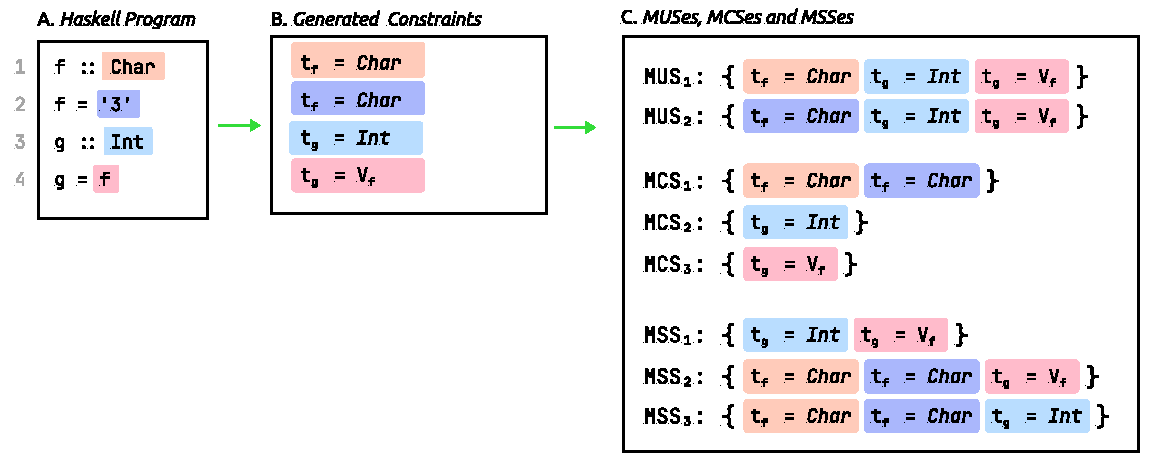
\includegraphics[width=\linewidth]{Subsets}
%   \caption{An example of generating constraints from Haskell program, and all the possible MUSes, MCSes, and MSSes can be acquired.}
% \end{figure}

\section{Three Classes of Type Error}
With the introduction of MUS, we can revisit the idea of three categories of type error we proposed in Chapter \ref{chap:introduction}. This categorization allows a formal study of the tools that are necessary to cover the information of a given type error. 

\subsection{Multi-step Type Error}
\begin{figure}[hbt]

  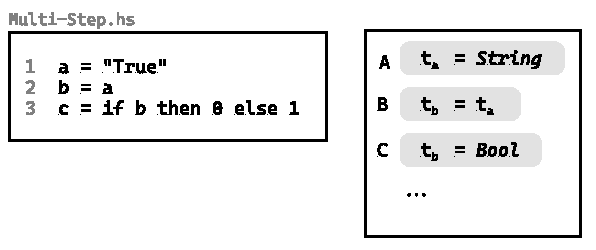
\includegraphics[width=0.5\linewidth]{Multi-Step-2}
  \caption{
    \label{fig:multi-step-2}
    A multi-step type error
  }
\end{figure}
Multiple-step type errors contain a chain of reasoning steps or a series of attempts to unify two logical terms. Multiple-step type error contains a single MUS. Each element of the MUS forms a singleton MCS. In the example of Fig \ref{fig:multi-step-2}, the MUS is the set of {A, B, C}. The MCSes are {A}, {B}, {C}. Removing any one of the MCSs will result in the program type check.

\subsection{Multi-witness Type Error}
\begin{figure}[hbt]
  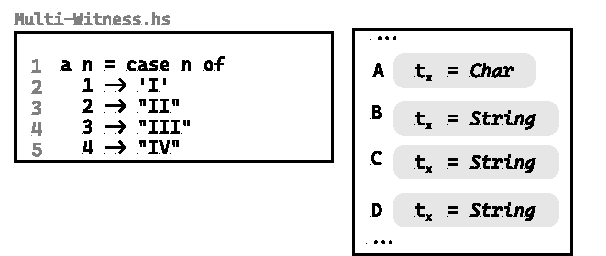
\includegraphics[width=0.5\linewidth]{Multi-Witness-2}
  \caption{
    \label{fig:multi-witness-2}
    A multi-witness type error
  }
\end{figure}

A Multiple-witness type error occurs when one side of the conflict contains multiple locations (witnesses) suggesting the same typing assignment. If one such location is removed, the type error will remain. In the example (\ref{fig:multi-witness-2}), there are three MUSes: {A, B}, {A, C}, {A, D}. Therefore, this type of error cannot be succinctly represented by a single MUS. 

\subsection{Multi-party Type Error}
\begin{figure}[hbt]
  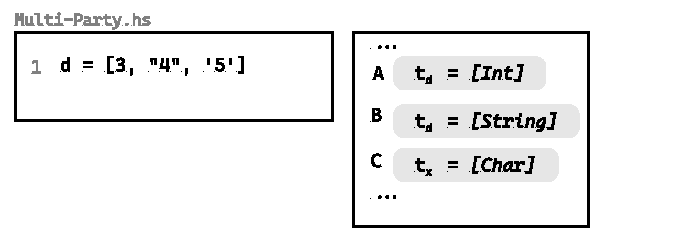
\includegraphics[width=0.5\linewidth]{Multi-Party-2}
  \caption{
    \label{fig:multi-party-2}
    A multi-party type error
  }
\end{figure}

A multiple-party type error is an error where multiple types of irreconcilable assignments can be obtained from locations in the source code. In the provided example  (\ref{fig:multi-party-2}), there are 3 MUS: {A, B}, {A,C}, {B,C}. Therefore, this type of error cannot be succinctly represented by a single MUS.

\begin{figure}[hbt]
  
  \includegraphics[width=\linewidth]{Compare}
  \caption{}
\end{figure}

\section{Conclusion}
In this chapter, we established a subset of the Haskell language by defining its syntax and typing rules. We explored two avenues to type-check a program in such language and obtain principle types: using the Hindley-Milner type system and using a constraint-based type system. In addition, we explored some type error analysis tools that are enabled by using a constraint-based type system and how these tools are applied to three different kinds of type errors. We will explore them in the next two chapters.
 
\graphicspath{{Figures/Chameleon}}

\chapter{Chameleon: An MUS-based interactive type error visualization and explanation tool}


\label{chap:chameleon} 

In this chapter, we discuss the challenge of traditional tools for debugging type errors, in localization, language and bias-adverting. We introduce Chameleon, a type error debugging tool based on type error slicing and MUS. We discuss the design of Chameleon and its usage in example, and show that 1) Chameleon is able to address the challenges in traditional debugging tools, and 2) Chameleon's improvement over other slicing based tools.




% \todo{As above, would start with motivation of dynamically typed langs e.g. JavaScript, Pythjon popularity but issues this brings...
% }

Dynamically typed programming languages such as JavaScript and Python have risen in popularity in recent decades \cite{chatley_next_2019}. These languages present a low barrier of entry, especially to beginner programmers: they require no type declaration, variable types or object structures can be modified dynamically, and functions can deal with dynamic input using ad-hoc polymorphism and runtime reflection. However, studies show that dynamically typed languages negatively affect development productivity \cite{kleinschmager_static_2012}, code usability \cite{mayer_empirical_2012}, and code quality \cite{gao_type_2017, ray_large-scale_2017, meyerovich_empirical_2013}. They are often found to produce error-prone code \cite{chen_empirical_2020, wang_empirical_2015,xu_python_2016} and require strong programmer discipline to avoid pitfalls \cite{chen_empirical_2020}. For these reasons, many modern dynamically-typed languages have introduced static typing annotations as part of the core language features in recent years (e.g.\ \textit{TypeScript}~\cite{microsoft_javascript_nodate} and \textit{mypy}~\cite{mypy_mypy_nodate}).

Functional programming languages have long enjoyed rigorous type systems and expressive type-level features. Techniques such as type inference and algebraic types have been standard practice for decades in functional languages such as ML and Haskell, and more recently in multi-paradigm languages, such as Rust and TypeScript. Various type system advances were introduced in Haskell and ended up in mainstream languages years or even decades after, leading many to consider Haskell the ``type-system laboratory" \cite{hudak_history_2007}.  Type classes, an implementation of generic programming, were introduced to Haskell in 1988~\cite{hudak_history_2007}, and now can be found in most popular languages such as C\#~\cite{bill_wagner_constraints_2022}, Java~\cite{oracle_generic_2022}, and TypeScript~\cite{microsoft_documentation_2022}.

One crucial challenge of programming in statically-typed languages is that type errors can sometimes be difficult to resolve~\cite{tirronen_understanding_2015, hage_solved_2020}. In particular, they may point to locations that are not the root  causes of the type error, expose errors in cryptic language, or provide misleading fixing suggestions~\cite{wu_how_2017}.
% Compared to dynamic type systems, static type systems offer programmers opportunities to weed out a large number of errors at compile time (reducing the need for run-time debugging) and to increase usability~\cite{mayer_static_2012} and codebase maintainability~\cite{kleinschmager_static_2012}. In recent years, the programming community has seen a trend of migrating away from dynamically typed codebases due to the lack of maintainability and refactoring safety when systems reach large scale and complexity~\cite{chatley_next_2019}. These migration methods include the introduction of gradual type annotations (e.g., JavaScript to TypeScript or Python with mypy) or transition to a modern strongly-typed language (Scala, Rust, Haskell, PureScript, etc.). However, with dynamically typed languages (e.g., JavaScript, PHP, and Python) still being most peoples' formative experience with programming and with such languages now firmly entrenched in education~\cite{stackoverflow_stack_2022}, this transition may pose difficulties for programmers who lack experience writing type-safe programs.

% \todo{There are a lot of minor grammer fix-ups needed throughout...}
% Programmers find challenges in adopting typed languages in their practice. \todo{I think this statement is plain wrong myself... 
%  Need strong references to justify if going to say this to SE audience!:}They tend to be verbose, hard to learn and generate bad error messages. 
% One obstacle programmers face when using a statically typed language is understanding and resolving type errors~\cite{marceau_measuring_2011, tirronen_understanding_2015}, especially when dealing with modern type features such as polymorphic types and implicit typing. Studies show most statically typed languages produce unhelpful and even misleading type errors~\cite{}. Symptoms of bad error messages include cryptic language exposing internal constructs of the compiler and incomplete or wrong error locations. These usability issues pose challenges to learners and teachers of the languages. impede the wide adoption of statically typed languages, especially for programmers who are now accustomed to the mindset of writing un-typed programs.

This paper introduces \chameleon{}, an interactive type debugging tool for Haskell. It can visualize the relevant context of a type error: where it happens or could have happened and which parts of the code cause it. In addition, \chameleon{} allows programmers to interactively explore all the parts of code where multiple types can be inferred and to resolve ambiguity. The most noticeable features are the type compare tool (Section \ref{sub:type-compare}), the candidate expression card (Section \ref{sub:candidate-expression}), and the deduction step (Section \ref{sub:deduction-steps}). These features are integrated into a debugging environment and can be enabled or disabled separately based on the programmers' preferences and debugging needs. \chameleon{} is open-source and is available at ~\cite{anonymous_chameleon_2022}.  
% \todo{Introduce Haskell earlier?  Motivate WHY Haskell?} The current implementation of \chameleon{} targets the Haskell 2010 language standard. However, it is planned to extend it to support other programming languages using the same underlying ideas and techniques. Historically, Haskell has been a test bed for advanced language features, and it is common for features established in Haskell to be transferred to mainstream programming languages. 

% \chameleon{} uses underlying type inference algorithms adapted from the command-line tool, Chameleon, developed in 2005 \cite{chameleon}. As described in Section \ref{sec:typeinferenceengine}, Chameleon computes the Minimum Unsatisfiable Subset (MUS) \tf{Explain what mus is} of type constraints in order to identify a set of code locations where multiple types can be inferred. Compared to standard compiler messages, which arbitrarily report the first place a type conflict arises, Chameleon error messages give a lot more context to the programmer to help them correctly resolve the conflict to match the program's intent. However, the Chameleon system was never tested with users.  Therefore, the first contribution of this paper is to address the research question: \textit{Is a minimally interactive version of Chameleon's multipart type-conflict display more effective in supporting type error debugging than traditional error messages? } (Sections~\ref{sub:us1} and \ref{sub:us2}).

% After affirming that the information Chameleon provides is beneficial for more complex type errors, we ask \textit{Do programmers benefit from the interactive exploration of type error locations?} (Sections~\ref{sub:us3} and \ref{sub:us4}). We then explore \textit{How do programmers use the interactive exploration features to solve type errors?}  (Section~\ref{sub:us4}).


This paper makes the following contributions:
\begin{itemize}
\item We provide the design and implementation of the \chameleon{} to visualize the relevant context of a type error and allow programmers to explore and verify the error locations in small chunks interactively.  
\item {
    We report the results of three experiments designed to evaluate \chameleon{}.}
\end{itemize}

Our experiments showed that programmers using \chameleon{} fix type errors faster than with traditional text-based error messages. This difference is more significant when solving harder tasks. Further, programmers who actively use \chameleon{} interactive features fix type errors faster than simply reading the type error output. Although \chameleon{} is designed to work with
the Haskell language, we plan to extend the underlying ideas to work with other strongly typed languages, such as Rust or TypeScript..

\section{Motivation}
The design requirements of \chameleon{} are motivated by limitations of traditional type errors, as documented in a number of studies (e.g.~\cite{Yang2000-wn, Hage2020-hg}), but which we illustrate here with a few motivating examples. 
%These limitations are sourced from the authors' frustration in teaching and writing Haskell. This list of shortcomings of traditional type errors is also strengthened by multiple studies pursuing improvement\cite{yang_improved_2000}. 

\begin{figure}[ht]
    \centering
    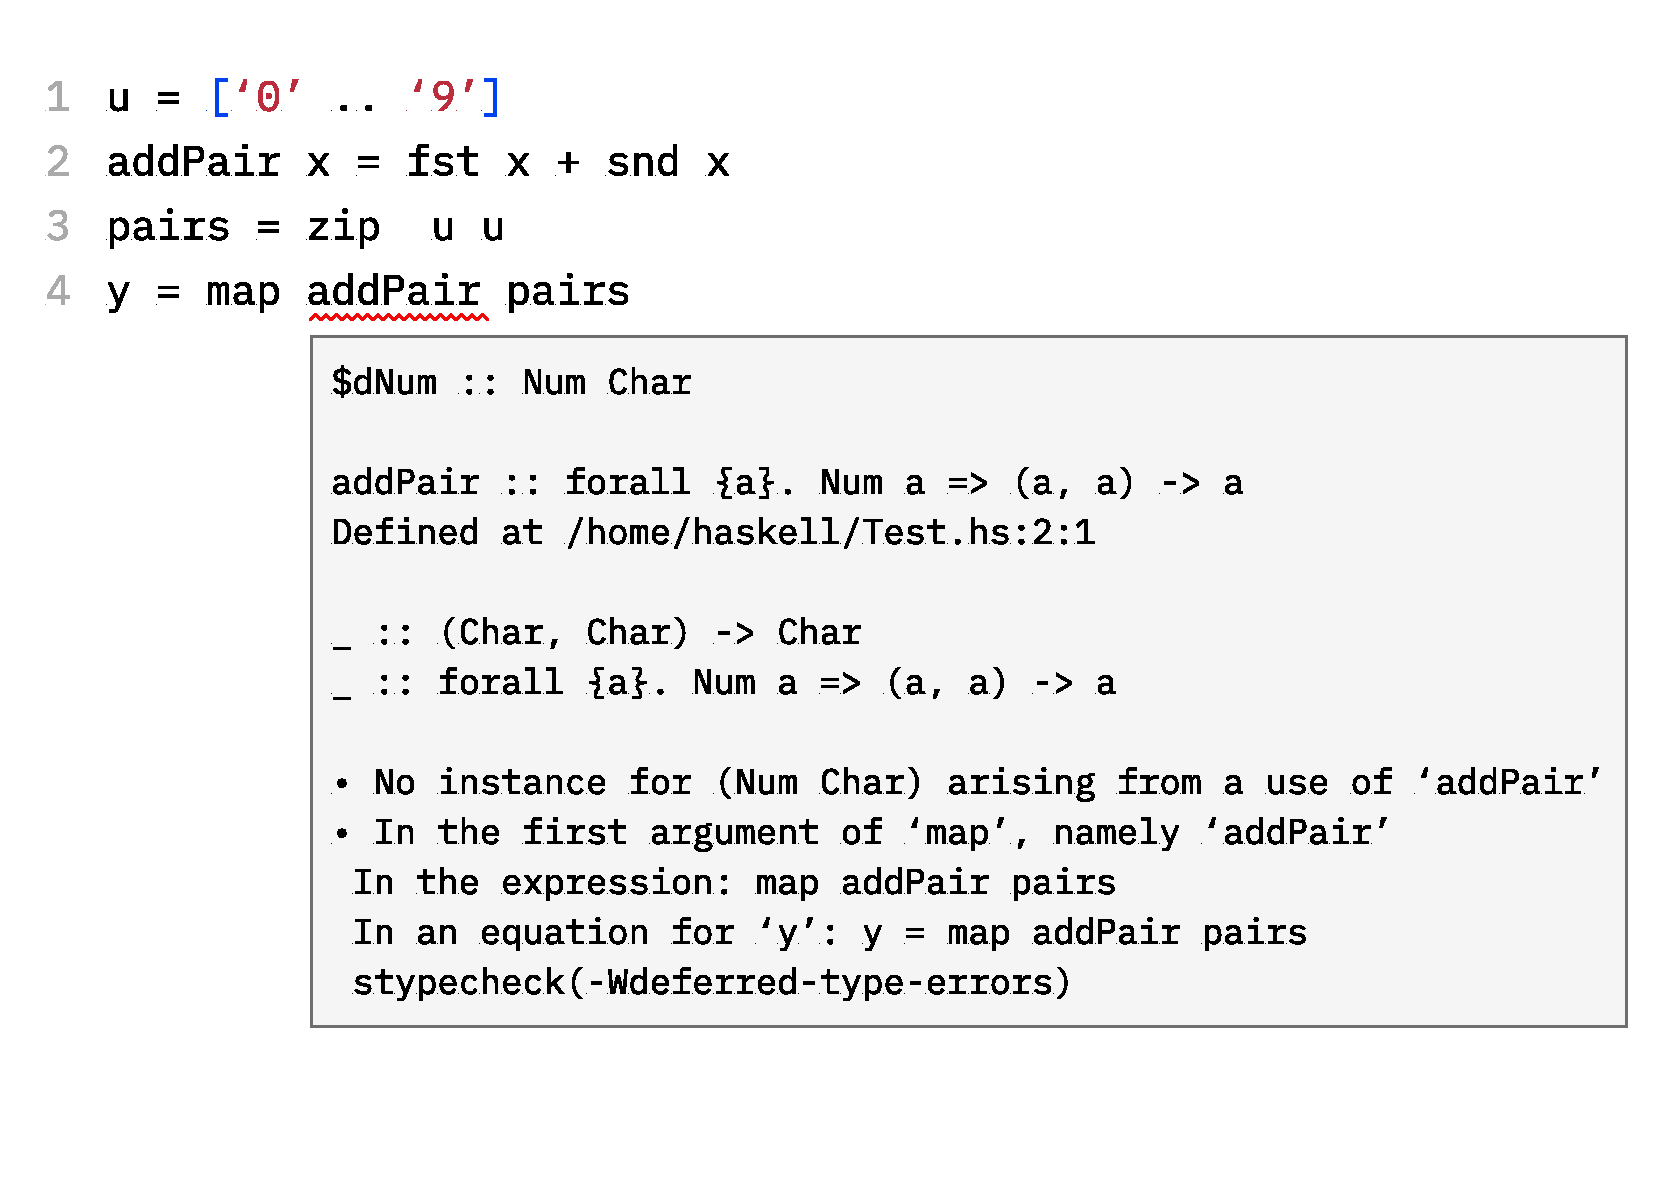
\includegraphics[width=\linewidth,trim=0mm 35mm 0mm 0mm]{images/add-pair-example.pdf}
    \caption[A type error displayed in Visual Studio Code and the Haskell Vscode extension]{
    A type error is displayed in Visual Studio Code\cite{Microsoft_undated-hs} with the Haskell Language Server\cite{HLS-Developers2023-ot} support.
The expression \texttt{addPair} is blamed for causing the type error. This may not match the programmers' intention. 
    }
    \label{fig:motivation-example}
\end{figure}

\textbf{Traditional type errors show only limited location}
Haack and Wells~\cite{Haack2004-fr} noted that ``\textit{Identifying only one node or subtree of the program as the error location makes it difficult for programmers to understand type errors. To choose the correct place to fix a type error, the programmer must find all the other program points that participate in the error.}'' The type error in Fig.~\ref{fig:motivation-example} can be fixed in multiple locations. For instance  replacing \texttt{['0'..'9']} on line 1 with \texttt{[0..9]}, or replacing \texttt{fst x} and \texttt{snd x} on line 2 with \texttt {read (fst x)} and \texttt{read (snd  x)}. In the type error message, only the \texttt{addPair} expression on line 4 was blamed.  The whole context is visible in this small example, but it can become problematic in large programs where the lines contributing to the type error are far apart in the source code.

\textbf{Traditional type errors are biased}
A common form of bias happens when a type error is reported in one expression, but it can occur in multiple other expressions as well. In Fig.~\ref{fig:motivation-example}, the error message arbitrarily focuses on only \texttt{addPair}, while ignoring that the literals in the definition of \texttt{u} may be incorrect. %Technically, this results from the side effect of different unification orders of the internal type-checking technique and has no bearing on what the programmers think and expect. 
Another form of bias is that traditional type errors are often framed as conflicts between \texttt{Expected type} and \texttt{Actual type}. This framing is standard practice in most typed languages. However, what is \texttt{expected} and what is \texttt{actual} are a side effect of different unification orders rather than the intention of the programmer. In both forms, the error message may lead programmers to falsely believe the validity of parts of code and wrongly accuse others.

\textbf{Traditional type errors give poor explanations}

When the compiler typechecks a program, it generates a series constraints from the source code and search for a satisfiable model for these constraints. But the details of this process are hard to explain to users and are usually not reported by compilers. For the typical type error shown in Fig.~\ref{fig:motivation-example}, the evidence for the type error is gathered from the previous declarations. These have to be rediscovered by programmers using less rigorous methods. 

\subsection{Design Goals of \chameleon{}}
Based on the limitations of traditional type errors, we give the following design requirements for \chameleon{}:

\noindent\textbf{Show} all the possible locations where the type error happened or could have happened.

\noindent\textbf{Explain} type errors avoiding jargon and internal constructs of the type checker.

\noindent\textbf{Do not presume} which expression is to blame for the type error based on the order of computation or which possible type for an expression is `actual' or `expected'.


\section{Chameleon IDE} \label{chameleon}
\begin{figure}[ht]
    \centering
    \includegraphics[width=\textwidth, trim=0mm 10mm 0mm 0mm]{images/atonomy.pdf}
    \caption[The anatomy of \chameleon{}]{
        \textbf{The anatomy of \chameleon{}.}
        The editor pane (left) is similar to a traditional code editor. Fragments of source code may have a highlight
        color (A). Additionally, an explanation layer (B) displays if deduction steps are enabled. The debugging pane contains three blocks. First, the error statement block contains an error statement (D), optionally, a list of candidate expression cards (E), a list of deduction steps (F), and a control bar (G) to increment/decrement deduction step. Second, the conflicting types block shows two alternative types (H). Third, the relevant type information block shows additional information (I) that may help understand type errors.
    }
    \label{fig:anatomy}
\end{figure}


\chameleon{} comprises two parts: a type inference engine and a novel interactive debugging interface. 
% This separation of concerns allows us to (1) adapt \chameleon{} into multiple front ends, such as IDE extensions, desktop applications, and web applications; and (2) reuse the debugging interface for different programming languages by replacing the back-end type inference engine. 
The debugging interface is designed from the ground up; the type inference engine is a re-implementation of the original Chameleon with several novel improvements, as described in Section~\ref{sec:typeinferenceengine}.

% \todo{I wonder about a high level overview diagram of tool / usage of tool, then the details of each component?}

% \todo{Can you use this example in Motivating Example sectoon (see my comment above) then use it to explain tool in this section?  Make sense?

% Is this example too simple...?}

\subsection{The Debugging Interface}

The \chameleon{} debugging interface provides three main features to visualize and explain type errors.

% the relation between the error statement and locations in code and to explore the explanation of each error location given by the type inference engine. 
%Further, programmers  can turn on and off features to suit their preferences and debugging needs.


\paragraph{Type compare tool} \label{sub:type-compare}
% In designing \chameleon{}, we want to argue against the practice of reporting type errors as the conflicts between \texttt{Expected type} and \texttt{Actual type}. Technically, the two alternatives are merely the side effect of different unification orders of the internal type-checking technique and have no bearing on what the programmers think and expect. 

The type compare tool shows conflicting types in different colors, each type associated with one or more error locations highlighted in a matching color (Fig.~\ref{fig:compare}).  
%The type error must be fixed by modifying at least one of these locations. 
%Error locations are highlighted with the matching color of the conflicting types. The type compare tool is useful to quickly bisect the type error. 
If the programmers know the expression's intended type (they usually do), they will be able to eliminate half of the possible locations. 
%To make this bisecting effect more pronounced, a user can hover over one of the possible types and only show the relevant locations that contribute to that type. 
A hover interaction over one of the possible types facilitates such bisection, causing only the relevant locations that contribute to that type to be highlighted. 
%This is a convenient way to put the error \emph{under the spotlight}.


\begin{figure}[ht]
    \centering
    \includegraphics[width=\linewidth, trim=0mm 10mm 0mm 0mm]{images/intro-compare-2.pdf}
    \caption[\chameleon{} with type compare tool enabled]{
        \textbf{\chameleon{} with type compare tool enabled}. \chameleon{} identified the conflicting types for the expression \texttt{u} and associated the relevant locations with each type. Compare the output with the traditional type error message in Fig.~\ref{fig:motivation-example}.
}
    \label{fig:compare}
\end{figure}

\begin{figure}[ht]
    \centering
    \includegraphics[width=\linewidth, trim=0mm 10mm 0mm 0mm]{images/intro-candidate.pdf}
    \caption[\chameleon{} with candidate expression cards enabled.]{
        \textbf{\chameleon{} with candidate expression cards enabled.}
        Indicates the type error can occur in the definition of \texttt{x} or \texttt{y}.
    }
    \label{fig:expression}
\end{figure}


\begin{figure}[ht]
    \centering
    \includegraphics[width=\linewidth, trim=0mm 10mm 0mm 0mm]{images/intro-deduction.pdf}
    \caption[\chameleon{} with deduction steps enabled]{
        \textbf{\chameleon{} with deduction steps enabled.}
        \chameleon{} explains the type error in four steps. In the screenshot, the active step is step 2, where \chameleon{} shows that the expression \texttt{x} and \texttt{y} should have the same type. 
    }
    \label{fig:deduction}
\end{figure}



\paragraph{Candidate Expression Cards}  \label{sub:candidate-expression}


% We propose candidate expression cards to make it clear to the user that there are multiple ways to resolve a type conflict. By contrast,  standard compiler error messages such as those of GHC arbitrarily focus the users' attention on only one candidate expression, e.g.\ ``\textit{Couldn't match expected type ‘Char’ with actual type ‘Bool’ in expression x}" where x is the candidate expression. In practice, this candidate expression often does not match programmers' intention (Fig.~\ref{fig:single-candidate}).  
A candidate expression is an expression that can be inferred to have two conflicting types. 
When a type error is detected, \chameleon{} provides a list of all candidate expressions, and programmers are free to choose the problem to resolve by clicking on one candidate expression card. In the example shown in Fig.~\ref{fig:expression}, \texttt{x} and \texttt{y} are both candidate expressions. Fixing either type error can make both expressions well-typed.


% This feature can be effective in resolving the problem that traditional tools tend to report errors that happened in source code from third-party libraries. With candidate expression cards, a programmer can freely change the context of the type error to the user-defined variables and functions to gain a better understanding of why their own code does not match the library code instead of the other direction.


Programmers select a candidate expression card by clicking on one card. Once a card is selected, the information in the conflicting types block changes to reflect the change of candidate expression. In the editor pane, some error locations change highlight colors based on the updated candidate expression. Alternatively, programmers can preview the change of a candidate expression by hovering on one card. The hover effect is reverted once the cursor moves away. 


\paragraph{Deduction steps}  \label{sub:deduction-steps}

% Deduction steps are motivated by the lack of explaining why the program has type errors. When the compiler rejects a program, it dumps the internal state of type checking.  This information may be a result of complex computing but this process is not reported by compilers. For a typical type error shown in Fig.~\ref{fig:ghc-error-example}, clearly, the evidence for the type error is gathered from the previous two declarations. These have to be rediscovered by the programmers again, using harder and less-sound methods. 

% \begin{figure}
%     \centering
%     \includegraphics[width=\linewidth]{images/ghc-error-example.png}
%     \caption{
%         }
%     \label{fig:ghc-error-example}
% \end{figure}

Deduction steps allow programmers to explore all the error locations one at a time (Fig.~\ref{fig:deduction}). Steps are shown as a list of sequentially  numbered circular buttons (step buttons) and an explanation layer in the editor window. In the explanation layer, the two locations under examination are outlined, and a line is drawn to connect these two locations. This line is accompanied by a human-readable text explanation of their semantic connection. Programmers are free to activate any step. The active step is shown in green. When activating a step, some highlights switch color. The message in the explanation layer changes accordingly. A program in Fig.~\ref{fig:deduction} generates a list of steps shown in Fig.~\ref{fig:step-interface} left.


Programmers can use mouse and keyboard shortcuts to increment or decrement the step number or jump to any step. Programmers resolve type errors by navigating through all the deduction steps and verifying whether each explanation aligns with their intention. Eventually, they will find a step that does not match, and the type error can be fixed by modifying one of the two outlined locations.

\begin{figure}[ht]
    \centering
    \includegraphics[width=\linewidth, trim=0mm 0mm 0mm 0mm]{images/step-explain.pdf}
    \caption[Deduction steps if they are shown all at once]{
Deduction steps if they are shown all at once. In practice, steps are shown one at a time. Programmers increment or decrement the step number using the step control bar (Fig.~\ref{fig:anatomy}-G) or by directly clicking on a step button (Fig.~\ref{fig:anatomy}-F). To increment or decrement the deduction step can be intuitively thought of as moving the position of the \textit{splitting point} (dotted lines) where the blue and orange highlights divide.
        }
    \label{fig:step-interface}
\end{figure}

Internally, deduction steps are different ways to divide the error locations into two  groups, denoted by the two colors. Each color infers a different type of the candidate expression. Each increment/decrement of the step changes the splitting point (dotted lines in Fig.~\ref{fig:step-interface}) of the two colors. Deduction steps are an interactive view of multi-step type errors.


\paragraph{Multiple Modes}

Nielson pointed out  that the two most important issues in designing for usability are understanding the users' tasks and the differences in users \cite{Jakob_Nielsen1994-gd}. From analyzing how users use \chameleon{}, we realized that the ideal debugging interface should adapt to the specific programmer and programming task. There are cases where a programmer wants the debugger to simply ``show the answer", and others to dive deeper into the problem domain and search for the optimal solution. To accommodate the need to customize the level of information density and granularity of control, \chameleon{} provides three modes: basic, balanced, and advanced. Programmers can switch between modes by clicking on the mode switching toggles (Fig.~\ref{fig:anatomy}-C). The features accessible from different modes are summarized in Table~\ref{tab:chameleon-features}.%shown in table~\ref{tab:chameleon-features}.

\begin{table}
    \centering
\begin{scriptsize}
\begin{center}

    \begin{tabular}{ l l }
     \textit{Mode} & \textit{Features} \\ \hline
     Basic Mode  & Type Compare Tool \\ \hline
     Balanced mode & Type Compare Tool  \\
     & Candidate Expression Cards  \\  \hline
     Advanced mode & Type Compare Tool  \\
     & Candidate Expression Cards \\
     & Deduction Steps  \\
    \end{tabular}
    \end{center}
\end{scriptsize}
    \caption{\chameleon{} modes and features}
    \label {tab:chameleon-features}
\end{table}


\subsection{The Type Inference Engine}
\label{sec:typeinferenceengine}

Chameleon was originally a command-line tool developed in the early 2000s to improve type error reporting %and introduced a design for interactive type debugging 
for the Haskell programming language.
Unlike traditional type errors produced by the Glasgow Haskell Compiler (GHC)~\cite{Gamari_undated-zu}, which uses a Hindley–Milner type inference system, Chameleon infers types using constraint solving. In Chameleon, constraints are generated from the source code based on typing rules. In addition, each constraint is labeled with the location where it is generated. This set of constraints is consistent if the program is well-typed and inconsistent otherwise. When a type error occurs, an efficient algorithm is used to derive a minimal subset of the constraints that still contain inconsistencies. This subset is called a Minimal Unsatisfiable Subset (MUS). From this, Chameleon can report a list of locations, using the labels of constraints that are in the MUS. Stuckey, Sulzmann and Wazny showed that program locations linked to the constraints from an MUS are all relevant to the type error and must include the cause of the error~\cite{Stuckey2003-pz}.

Despite successfully borrowing the underlying ideas, we could not reuse the original implementation of Chameleon since the project language standard and libraries used were out of date. 
\chameleon{} implementation extends the original Chameleon approach in a number of ways. \chameleon{} supports the base language of Haskell2010~\cite{Simon_Marlow2010-lg}. However, \chameleon{} does not support any advanced language extensions, such as GADTs.
%In addition to what Chameleon can do, a few new type inference features were added in the \chameleon{} implementation.



\paragraph{Recovering concrete types from type errors}


Using only constraints from the MUS is sufficient to locate the type error, but to recover types from type errors we need constraints from parts of the program that are irrelevant to the type error.  For instance, consider an ill-typed 2-tuple where two possible types can be assigned: \texttt{(Int, Int)} and \texttt{(Int, String)}. The types reconstructed from Chameleon may be \texttt{(a, Int)} and \texttt{(a, String)}. Although the recovered types are theoretically correct, they introduce the notation \texttt{a}, which denotes a generic type variable that can be any type, making the error message harder to understand. To solve this issue in \chameleon{}, for each constraint \texttt{c} in the MUS, we find a maximally satisfiable subset (MSS) from all the constraints that contain every other element of MUS but not \texttt{c}. These maximally satisfiable subsets, while not helpful in error localization, will produce the most concrete types, see Fig.~\ref{fig:compare-to-original}. Concrete types, such as \texttt{Int} and \texttt{String},  often provide extra information to programmers. With a type of \texttt{(Float, Float)}, programmers may want to convey a point in 2D space. However, a type of \texttt{(a, Float)} does not preserve such information.


\begin{figure}[ht]
    \centering
    \includegraphics[width=\linewidth, trim=0mm 6mm 0mm 0mm]{images/compare-to-original.pdf}
    \caption[Comparison between original Chameleon and \chameleon{}]{
Reporting the same type error, Chameleon uses more abstract types
\texttt{Int -> a} and \texttt{Char -> a}, while \chameleon{} uses the 
concrete types (types that do not contain type variables) \texttt{Int -> Bool} and \texttt{Char -> Bool}.
    }
    \label{fig:compare-to-original}
\end{figure}

 
% If the types get too verbose for programmers to identify the conflict between the two signatures, it is always possible to mute the overlapping information and highlight the differences from the debugging front end.


\paragraph{Type error explanation}

In addition, \chameleon{} provides support for type explanation. Similar to the type explanation system  in ~\cite{Jun2002-xp},  \chameleon{} is able to produce a human-readable explanation, but for type errors. This is achieved by annotating nodes in the abstract syntax tree with constraints and the type inference rules used. We generate an inference history from constraints and accompanying annotations. 


% \begin{lstlisting} [
%     language=Haskell, caption={
%     A simple program that is ill-typed. This program generates two constraints from line 1 and one constraint from line 2.
% }, label={listing:ifelse}
% ]
% if a then b else c
% a = "True"
% \end{lstlisting}


\begin{figure}[ht]
    \centering
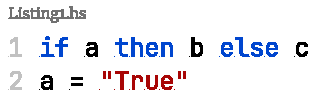
\includegraphics[width=0.4\linewidth]{images/Listing1.pdf}
    \caption[An example to illustrate constraint generation in \chameleon{}]{A simple program that is ill-typed. It generates two constraints from line 1 and one constraint from line 2. }
    \label{fig:listing1}
\end{figure}

For instance, for the program in Fig.~\ref{fig:listing1}, \chameleon{}  generates the following constraints and labels (in brackets) $T_a = Bool$ (if condition), $T_b = T_c$ (if branches), $T_a= String$  (definition). Clearly, as $T_a$ can not unify with both \textit{Bool} and \textit{String}, this program is not well typed. \chameleon{} can construct a human-readable explanation from the MUS. An example output for Fig.~\ref{fig:listing1} can be: \texttt{a} has type \texttt{Bool} because \texttt{a} is the condition of an if statement; however, \texttt{a} has type \texttt{String} because \texttt{a} is defined as the string literal \texttt{"True"}. This explanation facilitates the deduction steps (Section~\ref{sub:deduction-steps}). 







\section{Walkthrough} \label{sec:walkthrough}
In this section, we showcase \chameleon{} by walking through examples of its
use. The examples are given from the perspective of a hypothetical Haskell 
programmer Maxine. 

% \todo{A bit of redundant/repeated here c.f. prev section - if this is Usage example, again use motivating example in it?}

\subsection{Basic mode} \label{sub:basic}
Maxine writes a function to calculate the sum of a list of
numbers, but \chameleon{} shows there is a type error (Fig.~\ref{fig:basic-mode-1}). 
After reading the error reports, Maxine realizes that the error revolves 
around the expression \texttt{xs}. That is: \texttt{xs} can be
either \texttt{[a]} or \texttt{Int}. By matching the color in the
conflicting type block (Fig. \ref{fig:anatomy}-H) and the highlighted error locations 
Maxine knows that the \texttt{[a]} results from the pattern matching of the
\texttt{:} operator, while \texttt{Int} results from using \texttt{+} to
 add two expressions. 

\begin{figure}
        \centering
        \includegraphics[width=\linewidth,trim=0mm 8mm 0mm 0mm]{images/basic-mode-1.pdf}
        \caption{
            Maxine's code to calculate the sum of a list of integers;
            \chameleon{} reports an error on the expression \texttt{xs}.
            }
            \label{fig:basic-mode-1}
\end{figure}

% \begin{figure}[h]
%         \centering
%         \includegraphics[width=\linewidth]{images/basic-mode-2.pdf}
%         \caption{
%        Hovering on possible type 1 will limit the highlights 
%        in the editor to only the ones (in orange) that support \texttt{x::[a]}.
%         }
%         \label{fig:basic-mode-2}
% \end{figure}

% \begin{figure}
%         \centering
%         \includegraphics[width=\linewidth]{images/basic-mode-3.pdf}
%         \caption{
%             Hovering on possible type 2 (Fig. \ref{fig:basic-mode-2}-3) will limit the highlights 
%             in the editor to only the ones (in blue) that support \texttt{x::Int}.
%         }
%         \label{fig:basic-mode-3}
% \end{figure}





At this point, Maxine knows the possible type 1 aligns with her intention, and therefore, the error locations with blue highlights must be erroneous. After examining the program, it comes clear that Maxine forgets to apply the \texttt{sum} function recursively at the right-hand side of the addition. 


\subsection{Balanced mode} \label{sub:balanced}


Maxine writes additional code to add only even numbers in a list of integers, reusing the \texttt{sum} function she wrote earlier. After saving the file, \chameleon{} shows a type error in the expression \texttt{sum} (Fig.~\ref{fig:balance-mode-1}). However, this is not helpful because Maxine has just verified the implementation of \texttt{sum}. Switching to balanced mode, \chameleon{} shows two cards: \texttt{sum} and \texttt{evens}. 

\begin{figure}
        \centering
        \includegraphics[width=\linewidth,trim=0mm 8mm 0mm 0mm]{images/balanced-mode-1.pdf}
        \caption{
            Maxine's code to calculate only the sum 
            of even numbers. \chameleon{} reports 
            an error with two candidate expressions.
        }
        \label{fig:balance-mode-1}
\end{figure}


\begin{figure}
   \centering
        \includegraphics[width=\linewidth,trim=0mm 8mm 0mm 0mm]{images/balanced-mode-2.pdf}
        \caption{
            Clicking on the \texttt{evens} card (5) results in the changes in the
            conflicting types panel to show the possible types for \texttt{evens},
            and the changes highlight color to reflect the assumption that the
            definition of \texttt{evens} is the cause of the error.  
        }
        \label{fig:balance-mode-2}
\end{figure}

Maxine therefore clicks on the \texttt{evens} card and \chameleon{} reports two
possible types for the expression \texttt{[Int]} and \texttt{[Int] -> [Int]}
(Fig. \ref{fig:balance-mode-2}). Knowing the expression \texttt{evens} holds
a temporary list of even integers (hence it is of \texttt{[Int]} types), Maxine
concludes that the Possible type 2 is unintended. The locations with blue highlights must
contain the cause. It does not take long for Maxine to realize the list 
\texttt{l} is not supplied to the \texttt{filter} function.


\subsection{Advanced mode}  \label{sub:advanced}



\begin{figure}
        \centering
        \includegraphics[width=\linewidth,trim=0mm 8mm 0mm 0mm]{images/advanced-mode-1.pdf}
        \caption{
            Maxine's code to calculate only the sum 
            of even numbers in advanced mode. 
            The current step is step 5, \chameleon{} 
            explains that the two appearances of expression 
            \texttt{evens} should have the same type.
        }
        \label{fig:advanced-mode-step5}
\end{figure}

\begin{figure}
        \centering
        \includegraphics[width=\linewidth,trim=0mm 8mm 0mm 0mm]{images/advanced-mode-2.pdf}
        \caption{
            In step 6, \chameleon{} 
            explains that \texttt{evens} is defined as
            the expression \texttt{filter isEven}. The left-hand side
            and the right-hand side should have the same type.
        }
        \label{fig:advanced-mode-step6}
\end{figure}

\begin{figure}
        \centering
        \includegraphics[width=\linewidth,trim=0mm 8mm 0mm 0mm]{images/advanced-mode-3.pdf}
        \caption{
            In step 7, \chameleon{} 
            explains that \texttt{filter} is applied to 
            the function \texttt{isEven}. Assisted by 
            the type of \texttt{filter} in the 
            Relevant Type Information panel on the bottom
            right, Maxine can find the type error that 
            \texttt{filter} expects two arguments but receives one.
        }
        \label{fig:advanced-mode-step7}
\end{figure}

% For the task shown in section \ref{sub:balanced}, if Maxine is not satisfied by
% the options provided by \chameleon{}, by switching to advanced
% mode, she has access to the debugging steps. 

To illustrate the deduction steps with the task shown in section \ref{sub:balanced},  first, Maxine clicks on step 5 (Fig. \ref{fig:advanced-mode-step5}) and verifies
that the two occurrences of \texttt{evens} are supposed to be identical, and the
second use means \texttt{evens} is a list of integers. Second, she
clicks on step 6 (Fig. \ref{fig:advanced-mode-step6}) and verifies that
\texttt{evens} should be the same type as the declaration on the right-hand
side. 


Lastly, Maxine clicks on step 7 (Fig. \ref{fig:advanced-mode-step7}), and
it shows that the \texttt{filter} function is applied to one argument
\texttt{isEven}. By consulting the relevant type information, Maxine identifies
that \texttt{filter} is expecting two arguments while only one is provided. 


\section{Evaluation}

We conducted three user studies, iteratively refining the \chameleon{} UI and evaluating several research questions as per Fig.~\ref{fig:timeline}. 
%The number of participants and their Haskell experience, as well as key research questions and conclusions, were shown in figure \ref{fig:timeline}. \todo{Explain was a user study of the tool with practitioners?}


\begin{figure}
    \centering
    \includegraphics[width=\columnwidth,trim=30mm 35mm 35mm 5mm]{images/timeline.pdf}
    \caption{The timeline of \chameleon{}  evaluation.}
    \label{fig:timeline}
\end{figure}

\subsection{Experiment Design}
\subsubsection*{\textbf{Recruitment}}

Participants were recruited via the Reddit \textit{r/haskell} and \textit{r/programminglanguages} communities. 
%Recruiting from social media allowed us to access a more diverse demographic that better represent the true population of Haskell programmers. 
Participation is fully anonymized; detailed ethical implications of these experiments are reviewed and approved by the IRB of the authors' institution.


\subsubsection*{\textbf{Experiment setting}}
Experiments were conducted online and unsupervised. 
%Participants took the study online via a web browser and at the physical venue of their choosing. 
All user studies use a web-based debugging environment developed by the authors. 
%Conducting the studies online helped us avoid variation when performing tasks in unfamiliar places and using different setups. 


\subsubsection*{\textbf{Training and group assignment}}
After consent, participants received interactive training on the tool interface and interactive features. Participants were also shown a cheat sheet summarizing the key functionality of the interface, and had access to the cheat sheet at all times during the study. Participants were given 4 trial runs (2 for each setting) before the data collection started. 
All the studies used a within-subject design to evaluate the effectiveness of different tools or feature sets while counterbalancing the difference in programming proficiency between participants. In each study, participants were required to complete a series of programming tasks (8 for studies 1a and 1b, 9 for study 2). At each task, a participant receives a single Haskell file that contains one or more type errors. They were then asked to correct the code with the help of the given tool.


\subsubsection*{\textbf{Data Collection}}
Time is measured from the start of each task to the first time the program is successfully type-checked and also passes all the functional tests. Participants are able to skip a task if they are stuck. 
% The data is automatically recorded by the online debugging environment. To not introduce a barrier to completing the study, every task can be skipped if the participant made three failed attempts or is stuck for over 1 minute on the task.
After completing all tasks, participants are prompted to complete a debriefing survey. The survey questions include their Haskell experience and feedback on the tools.

We used a browser session recording tool~\cite{openreplay_openreplay_2022} to record the study sessions. This allows us to identify usability issues in the study and to recognize general patterns. 
%The reason we found this format inferior is that the recording technology does not provide a high enough sampling rate for us to be confidently used for rigorous analysis.
%One use of the session recording is for outlier trimming.  We identify participants who left the computer for an extended period of time. We first ran a statistical analysis to identify the long gap (2 standard deviations) between actions using program logs for each participant. Then, we manually checked with the session recording to verify there was actually no user input (mouse movement, scrolling). 

\subsection{\chameleon{} Human Studies}

\subsubsection{\textbf{\chameleon{} 1}}  
An earlier version of the UI than that depicted in Figs.~(2-13), it featured the type inference engine that recovers most concrete types after type errors occur and a minimal set of debugging features. Key features in \chameleon{} 1 include showing two (or more) alternative types, showing all possible error locations, dividing possible error locations into groups based on alternative types, and concrete type restoration. In short, \chameleon{} 1 is equivalent to \chameleon{} 2 set to basic mode. 

% \begin{figure}[h]
%     \centering
%     \includegraphics[width=\linewidth]{images/chameleon-v1.pdf}
%     \caption{
%         \chameleon{} 1
%         }
%     \label{fig:chameleon-v1}
% \end{figure}

Two  studies (1a \& 1b) were conducted to compare the effectiveness of solving type errors using \chameleon{} 1 and GHC compiler error messages. We choose GHC compiler error messages as the baseline because it is the canonical tool for working with type errors in Haskell.
%Although high-level tools like Haskell Language Server exist, they generally relay the GHC error messages verbatim. 
% The procedure of these studies is shown in figure \ref{fig:procedure-1}.


Eight tasks were given in both studies. In study 1a, the tasks were taken from the exercises of the Haskell programming class in the authors' institute. In the second study, the tasks are sourced from the top 20 Haskell topics on GitHub~\cite{github_github_2022}. The authors then manually added type errors into the program. In both studies, the type errors include simple mismatch, confusing syntax, missing instance, precedence and fixation, infinite types, and confusing list versus element. These categories follow the common type errors in Tirronen's study \cite{tirronen_understanding_2015}. 

Studies (1a \& 1b) address the research question:

\noindent\textbf{RQ1.} \textit{Do programmers solve type errors faster with \chameleon{} than GHC compiler error messages?}


% \begin{figure}[h]
%     \centering
%     \includegraphics[width=\linewidth]{images/procedure-1.pdf}
%     \caption{\todo{Does this figure really help at all?}}
%     \label{fig:procedure-1}
% \end{figure}

% The study investigates the effectiveness of \chameleon{} compared to the GHC compiler error messages. We chose GHC compiler error messages as it is the canonical tool for debugging type errors in Haskell. Although high-level tools like Haskell Language Server exist, they relay the GHC error message verbatim for type errors. Participants are asked to complete 8 tasks. The tool participants used during each task alternated between \chameleon{} and GHC. Task programs were sourced from HaskellWiki \cite{haskellwiki}. The author manually added type errors. The errors cover a range of common Haskell type errors, including abstract data types, wrong arity, control expressions (if and case), infinite types, and tuples. The lines of code (LoC) range from 7 to 17 (mean = 11, median=10.5).


% In total 39 participants finished the study. Among them, 12 participants have over five years of Haskell experience, and 5 participants have three or four years of Haskell experience. And 8 participants have one or two years of experience, and 5 participants used Haskell for under a year. The rest left the question unanswered.

\begin{figure}
    \centering
    \includegraphics[width=0.8\linewidth,trim=15mm 12mm 15mm 35mm,clip]{images/user-study-1a.pdf}
    \caption{Study 1a task completion time (secs.) with 95\% confidence interval.}
    \label{fig:analysis-1a}
\end{figure}


\begin{figure}
    \centering
    \includegraphics[width=0.8\linewidth,trim=12mm 15mm 12mm 35mm,clip]{images/user-study-1b.pdf}
    \caption{Study 1b task completion time (secs.) with 95\% confidence interval.}
    \label{fig:analysis-1b}
\end{figure}

\subsubsection*{\textbf {Results}}

The data collected during study 1a, Fig.~\ref{fig:analysis-1a} does not show significant differences across Tasks 1-7. In hindsight, these tasks were trivial challenges for most users, and the individual differences among participants are generally more significant than the differences between treatments. However, one interesting observation is task 8, where the \chameleon{} group outperformed the GHC group. We attribute this significant difference to the difficulty of Task 8. The source file is longer and involves more language features (abstract data types and high-level functions). GHC struggles to produce a relevant error message for this type of error. 
From this result, we hypothesized that we might observe a more significant difference using tasks with lengthier and more realistic source code. 
This hypothesis is also supported by the most common feedback claiming that the tasks were too trivial to invite meaningful evaluation. One participant said, ``Looks nicer than GHC, but without trying it on something more complicated, I cannot conclude whether it would help me in practice." 

Therefore, in study 1b we introduced more difficult challenges and indeed observed that the \chameleon{} group was faster than the GHC group in almost all tasks (figure \ref{fig:analysis-1b}), barring task 1. A two-sample paired t-test was performed to compare the completion time between \chameleon{} and GHC groups. There was a significant difference between the two groups: $t(23) = -3.86, p = 0007$. For task 1, it is suspected that some participants spent more time exploring the interface of \chameleon{} due to its unfamiliarity. For all other tasks, from the video recordings, we saw many \chameleon{} users confidently skip reading unrelated chunks of code, while GHC users generally read through the whole program. In harder problems and messier code, we notice programmers start to report the benefits of \chameleon{}. ``It's most useful feature that I noticed was that it points out the locations of both conflicting uses; GHC often makes it difficult to figure out how it's coming to a conclusion about a type." reported one participant. ``I think \chameleon{}  does a much better job than GHC's error messages. I like that it shows the sources for the type judgments. This makes it quite easy to figure out how to rectify errors." reported another participant.

% \begin{itemize}
%     \item {It has a longer source file than other tasks (only shorter than task 6, but task
%     6 contains two independent type errors while task 8 is one connected task
%     error);}
%     \item {It is more complex than others (involves abstract data types and function application); and
%     }
%     \item {
%         GHC struggles to produce a relevant error message for this type of error.
%     }
%   \end{itemize}


  

% \begin{figure}[H]
%     \centering
%     \Description{A screenshot from user study 1}
%     \includegraphics[width=\textwidth]{round1-screenshot.pdf}
%     \caption{
% One participant working with \chameleon{}  managed to identify the most probable location of the error (the application of `fromMaybe'` on line 11) by hovering over the two alternative types. The participant then quickly realized that the first argument `0` (highlighted in orange) is inconsistent with the definition where it is case matched to a `Nothing` value (highlighted in purple). After two retries with short hesitation the participant found the correct fix (by reversing the order of `0` and `n`).
%     }
%     \label{fig:r1-task8}
% \end{figure}


% \begin{figure}[htb]
%     \centering
%     \Description{A screenshot from user study 1}
%     \includegraphics[width=\textwidth]{round1-screenshot-ghc.pdf}
%     \caption{
%         In task 8, participants using GHC took longer pauses at this task before committing to further investigation, either carefully reading the whole text or figuring out the meaning of the error message. The GHC error message is unfortunately unhelpful for this task.
%     }
%     \label{fig:task8-ghc}
% \end{figure}




\subsubsection{\textbf{\chameleon{} 2}}  \label{sub:us4}
Based on observations of Study 1 we introduced several new features to \chameleon{}, eventually resulting in the UI depicted in Figs.~(2-13). Interactive features were available in this iteration, such as deduction steps, candidate expressions, and mode switching. A few other user interfaces \cite{anonymous_interactive_2021} were designed and prototyped between the development of \chameleon{} 1 and \chameleon{} 2. Study 2 addresses the research question: 

\noindent\textbf{RQ2:} \textit{How do programmers use the interactive features in \chameleon{} 2?}. 

More specifically:
\begin{itemize}
    \item \textbf{RQ2.1} How do programmers use the advanced features provided by \chameleon{} 2?
    \item \textbf{RQ2.2} Do programmers prefer switching modes during debugging type errors?
    \item  \textbf{RQ2.3} What are programmers' preferences among the three modes provided by \chameleon{} 2?


\end{itemize}

During each run, the initial mode of each task alternated through the three different modes and repeated three cycles in nine tasks. The order of the three modes in each cycle is counterbalanced among all participants. However, participants can switch to other modes at any time. 



% \begin{figure}[h]
%     \centering
%     \includegraphics[width=\linewidth]{images/procedure-2.pdf}
%     \caption{\todo{Does this figure really help at all?}}
%     \label{fig:procedure-2}
% \end{figure}

\subsubsection*{\textbf{Results}} 

Study 2 is more exploratory in methodology than Study 1. We encouraged programmers  to discover their way of using the tool. In post hoc analysis of the collected log data, we were able to extrapolate some interesting patterns of how the tool was used. 


\textbf{RQ2.1}. The most striking feature of the data is that users tend to vary wildly in their use of the tool. Some users used the features extensively, while others completed the tasks without actively exploring the given information. Based on this discrepancy, we divided the users into three groups in table~\ref{tab:interaction-level}.
\begin{table}
    \centering
\begin{scriptsize}
\begin{small}
\noindent\begin{tabularx}{\linewidth}{ 
  | >{\hsize=.26\hsize}X 
  | >{\hsize=.74\hsize \raggedright\arraybackslash}X  | }
    \hline
        Interaction level & Description \\ \hline
        \textit{Minimal}  & Users completed the tasks by making changes in source code, type checking, and reading error messages. \\ \hline
        \textit{Low}  & Users only actively used universal features in all modes, for example, hovering on "Possible type 1" and "Possible type 2" to narrow down error space. \\ \hline
        \textit{High}  & Users did everything from the low interaction group but used features specific to the Balanced mode and the Advanced mode, such as activating steps and expression cards. \\ \hline
\end{tabularx}
\end{small}
\end{scriptsize}
    \caption{Levels of programmer interaction and their description}
    \label {tab:interaction-level}
\end{table}

As shown in  Fig.~\ref{fig:r4-analysis}, the time to complete each task roughly relates to the interaction level of participants. Participants with higher interaction levels generally performed better, and the lowest interaction level was worse. Tukey’s HSD Test for multiple comparisons found that the completion time was significantly different between the minimal interaction group and the high interaction group ($p \le 0.001$, 95\% C.I. = [18.26, 31.41]), and between the minimal interaction group and the low interaction group ($p \le 0.001$, 95\% C.I. = [11.96, 26.67]). The results from three tasks stand out from the general trend: in Tasks 4 and 6, higher interaction users performed worse, and in task 9, the general trend is exaggerated. As with Study 1a and 1b, this difference is likely related to task difficulty. Tasks 4 and 6 are shorter than other tasks. The ideal fixes for these two tasks are placed relatively early in the source code (both in the first two lines of the source code). Users simply reading top to bottom could quickly identify the error without needing to skip unrelated sections of code using the information provided by \chameleon{}. This reduced the apparent benefit of \chameleon{} in these tasks. On the other hand, task 9 is the lengthiest task of all. It also involves deeply nested type definitions that are harder to follow in mind.

\begin{figure}
    \centering
    \includegraphics[width=\linewidth,trim=0mm 15mm 0mm 50mm,clip]{images/user-study-2.pdf}
    \caption{Study 2 task completion time (secs.) with 95\% confidence intervals.}
    \label{fig:r4-analysis}
\end{figure}


% \begin{figure}[h]
%     \centering
%     \includegraphics[width=\linewidth]{images/r4-task9.png}
%     \caption{
% High interaction users were able to locate the exact line for a potential fix after navigating to deduction step 6 or 7, which directly revealed the true cause of the type error. After this, 12 out of 15 high interaction users provided the most ideal fix in the first try. Low interaction group  takes longer time to examine the problem, provided wrong fixes in the initial trials. One participant fixed a minor run-time issue (a problematic pattern matching of `[attributes]` on line 18) however failed to identify the culprit of the type error. This location is not pinpointed by \chameleon{} and therefore it is understandable that programmers who used the deduction steps would be able to ignore this part of the source code.
%     }
%     \label{fig:r4-task9}
% \end{figure}


Another observation is when using the mode switching feature of \chameleon{}, we show this by presenting the starting mode and finishing mode of each task and each participant in a correlation matrix (Fig. \ref{fig:r4-mode-switching}). This observation suggests two characteristics of using multi-mode debugging tools. First, to answer \textbf{RQ2.2} programmers are roughly splitted in this matter: 53\% changing modes vs. 47\% staying in the same mode. Second, to answer \textbf{RQ2.3} when changing modes, programmers generally switch to the more informative modes instead of the more concise ones.
\begin{figure}
    \centering
    \includegraphics[width=0.7\linewidth,trim=0mm 5mm 0mm 5mm,clip]{images/mode-switching.pdf}
    \caption{Study 2 mode switches by starting mode.  Users overwhelmingly switched to the more sophisticated interface mode.
        % The rows represent the finishing mode, columns starting modes.
    }
    \label{fig:r4-mode-switching}
\end{figure}


\subsection{Limitations}

One threat to the validity of the evaluation is the number of participants. Although for each study we received hundreds of online participants, the studies suffered from a high abandonment rate (especially study 1b). This was expected: the programming challenges are difficult, and our volunteer participants are unremunerated. 
Because we recruited participants online and anonymized all the participants, it is possible for participants of a previous study to enter a later one. This creates variation in familiarity. We offset this by using new code challenges in every study and conducting trial runs before data collection to bring new participants up to speed.
Conducting studies remotely and unsupervised left us no means to intervene when users encounter usability issues. To mitigate this, we conducted cognitive walkthroughs and sandbox pilots before running each study.

Future evaluation would benefit from using more realistic tasks. The tasks in our human studies do not get as complex as professional Haskell programmers may face in a typical production codebase. It would be interesting to see how \chameleon{} is used against type errors that span multiple files and packages and include more confusing abstractions, like Monads, Monad transformers, and Lenses.

\section{Discussion}

% \todo{Suggest try and strucuture this a bit more e.g. each para bold the key lesson @ start of para. Can you group into implications for research/implications for practice to make more actionable??}

This chapter presents the interactive type debugging tool \chameleon{} and charts the evolution of its design across several iterations in response to user evaluation and feedback, as well as examines the effectiveness of the general approach compared to traditional static type error messages. We found that programmers using \chameleon{} are able to debug errors faster than using traditional text-based error messages. This effect is shown more clearly when the task is not trivial. We found that programmers who actively use \chameleon{}'s interactive features are more efficient in fixing type errors than passively reading the type error output. In this section, we discuss a few interpretations of the results.


\subsection{Effect on Reading Source Code}
From the results of Study 1a, we observed that the choice of debugging tool had little effect on how fast programmers solve simple type errors. Conversely, when facing more realistic problems (longer source code, error locations more scattered) in study 1b, programmers are more effective using \chameleon{}. One explanation is that \chameleon{} reduces the amount of reading time by taking programmers more directly to the problem. Earlier studies \cite{Jbara2015-gr, Peitek2020-nb} showed that reading source code is generally the initial step of solving programming problems and is done in several passes. Although traditional compiler error message tools initially show fewer locations, these may be incomplete, meaning that programmers have to expand the reading span without clear guidance. In contrast, \chameleon{} shows more error locations initially. However, the completeness of error locations assures programmers which part of the source code can be safely skipped.

\subsection{Forming Debugging Plans}
From the results of Study 2, we found that programmers who use the interactive tool fix type errors faster than the ones who passively read the error output. This effect is stronger in harder tasks. We speculate that one factor of this result is that  \chameleon{} helps to develop debugging plans. We observed that when working with \chameleon{}, programmers form different debugging plans to attack the problem. Among the \textit{high} interactivity participants in user study 2, some programmers cycle through deduction steps as a guide to reading source code; some navigate to both ends of the deduction chain where types are normally grounded and concrete. In contrast, \textit{minimal} interactive participants generally form similar plans, including carefully reading the program text and manually annotating expressions based on their understanding of the program.


\subsection{Externalize Intermediate Typing Information}
We speculate another factor of the effectiveness of \chameleon{} interactive debugging tools is that they help programmers effectively chunk intermediate information. With the program shown in Fig.~\ref{fig:listing2}, \chameleon{} offers two candidate expressions: \texttt{f} can be typed as \texttt{Int -> Bool} or \texttt{Char -> Bool}; \texttt{z} can be typed as \texttt{Int} or \texttt{Char}. Although  these two statements are equivalent in theory, programmers are often required to compute the latter from the former or vice versa. And this computation may carry out multiple layers. Programmers have to remember all the intermediate types and their reasoning throughout such mental gymnastics. Assisted by candidate expression cards and deduction steps, this intermediate information is externalized on screen and can be retrieved anytime. A recent study on working memory \cite{Crichton2021-ru} suggested this approach may provide a positive effect in helping programmers manage cognitive load and free up working-memory space for high-level thinking.


\subsection{Exploreg Multi-step Type Errors}

\chameleon{} finds a single MUS, use each constraint inside the MUS to generate interactive debugging steps, allowing programmers to ``replay'' how type errors occured in a ``frame by frame'' fashion. This design presents the internal logic conflict faithfully to programmers, and aligns with our analysis of multi-step type errors in Chapter~\ref{chap:introduction} by visualizing the chain of logical inference and allowing programmers to interact with it. However, it is worth noting that \chameleon{} is not ideally designed to conquer multi-witness and multi-party type errors, due to its focus on a single MUS.

% \subsection{Implication for future studies}
% Our study aims to contribute to the wider understanding of program comprehension in the context of advanced type systems. One promising research area to extend our results is to apply the design of \chameleon{} to other languages with high demand for explainability\cite{ferdowsi_usability_2023}.

% Colorization and overlay widgets are used to visualize relations and orders that may not conform to the source code structures. These techniques fit well to types because the introduction and elimination of typing constraints tend to be scattered throughout the program. A interesting question is whether these techniques can also be applied to other program properties, such as memory allocation and freeing, as well as message dispatching and consumption, which also exhibit similar patterns.

% Finally, we employed MUS (minimal unsatisfiable subset) for fault localization and types recovery, but we are also curious about the possibility of further analysis based on MUS to power advanced debugging systems, such as efficient and accurate type error repair by combining our results with mutation testing or solution searching based on machine learning.

\begin{figure}[ht]
    \centering
    \includegraphics[width=0.4\linewidth]{images/Listing2.pdf}
    \caption{\chameleon{} reports an error in the expressions \texttt{f} and \texttt{z}}
    \label{fig:listing2}
\end{figure}

% \begin{listing}
% \begin{minted}[bgcolor=bg,linenos]{haskell}
% f z     
%     | z == 3 = False
%     | z == '4' = True
% \end{minted}
% \vspace*{-9mm}
% \caption{\chameleon{} reports an error in the expressions \texttt{f} and \texttt{z}}
% \label{listing:2}
% \end{listing}
% Implication for research
% In our studies, \chameleon{} shows a few different designs for type error visualization and interaction. However, we are far from exhausting the search space. One challenge we notice in the current design is that programmers have to shift their focus between the editor on the left and the \chameleon{} debugging interface on the right. Using the hover popup window in most mainstream IDEs may reduce the context switching during debugging.

% Integration with existing tools
% The current implementation of \chameleon{} requires non-trivial adaptation for editors such as VS Code and IntelliJ due to the overlay explanation layer. This type of error visualization is non-standard in mainstream editors. However, there may exist alternative representations of \chameleon{} error reporting using only the features available in major editors and IDEs. It is especially beneficial to represent \chameleon{} errors using a universal debugging middle layer such as language server protocol (LSP). This will allow \chameleon{}  to be adapted into various coding environments which support an LSP back end.


% Extend to other languages
% Our study focuses on the Haskell language for its popularity in the academic world. However, the low quality of textual type errors is a problem not limited to Haskell. Modern statically typed languages more or less all share the same problem. We believe the underlying type reporting technique and algorithms can be generalized to other languages. It will be exciting to see how interactive debugging features perform in other paradigms, such as  imperative languages and incremental type systems.

% Ranking candidate expressions and alternative types
% Our design of \chameleon{}  emphasizes allowing programmers to update the type error based on their prior knowledge. It unfolds to answer three questions: which expression should be considered ill-typed? Between multiple possible types, which one should be considered intended? Among all the possible locations, which one should be considered the cause? \chameleon{} answers all three questions by leaving them to the hands of the programmers. However, it is possible in situations, prescriptive error messages are preferred. Using heuristic methods may achieve the best of both worlds. It may produce effective results by guessing the possible un-typable expression based on the position it appears in the syntax tree and project structure or guessing the intended type signature by comparing the number of supporting slices in the source code.

\section{Related Work}

% \todo{I would do a short Motivating Example section straight after intro showing example of untyped lang, problems it brings, and outline requirments for the proposed IDE to address it. Make sense??}

% \todo{Do yoou need Related Work here - or put @ end of paper just before Summary - I tend to do the later now UNLESS its REALLY needed by reader - IMO could put @ end and get to your work/contributions much quicker}

\subsection{Finding all type error locations}
Many have studied the approach of finding all locations that contribute to a type error~\cite{stuckey_interactive_2003, haack_type_2004, pavlinovic_practical_2015, schilling_constraint-free_2012}. Type error slicing~\cite{haack_type_2004} is a technique that finds locations that are complete and minimal for the type error. Internally labeled constraints and Minimal Unsatisfiable Subset (MUS) generation are used to generate these slices. The language supported in Haack's work was a subset of Standard ML. The original Chameleon~\cite{stuckey_interactive_2003} used  Constraint handling rules (CHR) to support the computing of type error slices in Haskell. Chameleon also supported advanced type-level features (type classes and functionally dependent types). The project also introduced the ability to query type information through a command line interface. Although Chameleon was firmly grounded in results from type theory, its designs were never evaluated with user studies. While finding all error locations is useful in comprehending type errors, it is only 1 of the 7 properties listed in the proposed manifesto of good type error reporting~\cite{yang_improved_2000}.
To the best of our knowledge, ours is the first user-centered evaluation of an interactive type debugging system involving type-error slicing.


\subsection{Producing high-quality error explanation}
One weakness of compiler error messages, in general, is that they fail to explain the error in human language. As put in~\cite{barik_developers_2017}, ``Error messages appear to take the form of natural language, yet are as difficult to read as source code."  A well-studied approach to producing better error explanations is through ECEM (Enhanced compiler error message). Through a series of mixed-method studies, Prather showed~\cite{prather_novices_2017} that ECEM has a positive result in understanding compiler errors. Decaf~\cite{becker_effective_2016} is a tool that can rephrase Java compiler error messages into an enhanced version. In a study of over 200 CS1 students, Decaf was shown to reduce overall errors in their coding practices. Berik proposed a framework~\cite{barik_how_2018} for constructing compiler error messages based on argumentation theory, and showed that error messages following a simple argumentation layout or an extended argumentation layout are more human-friendly.  These works show the significance of improving the language in the compiler error messages. Most principles and suggestions are followed in \chameleon{} in constructing error statements. However, these earlier studies were not targeting type errors alone but general compiler errors (some even include runtime errors). The nuances of type errors, such as alternative typing, were not considered. Moreover, these explanation systems were designed specifically for novice users. 


% \subsection{Suggesting resolution}
% One direction to approach type error debugging is by suggesting solutions to fix the type error. Sheng Chen's works~\cite{chen_counter-factual_2014, chen_efficient_2020, chen_improving_2022} on counterfactual typing are able to suggest changes to make the ill-typed program type-check.  Lerner  studied an approach~\cite{lerner_searching_2007} of repeatedly modifying the AST (abstract syntax tree) and querying the compiler/type checker to know whether the new program is well-typed. This approach allows the algorithm to suggest syntax changes that could fix the type error. Benefiting from not needing a type system implementation and being language agnostic, the underlying idea was implemented and evaluated in two different languages with ten university students. While suggesting syntax changes is very intuitive in practice, this approach has limitations for teaching and learning purposes, as it is not able to explain why the type errors occur and why fixes are suggested. The lack of explanation is due to the inquiry into the underlying type-check being a binary state. Deep type-level analysis (typing rules and language features) was not communicated to the inference algorithm.


\subsection{Interactive Debugging}
% The original Chameleon provides a certain level of ``interactive'' debugging through a command-line interface~\cite{stuckey_interactive_2003}, allowing the programmer to query different parts of the program. A recent study \cite{tsushima_type_2021} provided an interactive type debugging system that restores type information based on the output from CFT (Counter-factual typing)~\cite{chen_counter-factual_2014, chen_efficient_2020, chen_improving_2022} inference. Both tools allow programmers to change their assumptions about which expression is ill-typed. While both tools show a strong influence on theoretical development, they were not evaluated in realistic studies with human participants. In addition, command line-based debugging tools suffer the same limitation as other line-based tools, namely, limited user interaction, limited graphic capability (ANSI text), and the requirement of remembering the command language. 


Modern programming tools can offer alternative methods of code authoring, display real-time feedback and reveal complex programming contexts through visualizations. Many tools aim to improve the debugging experience using such capabilities. We list two. Hazel Tutor \cite{potter_hazel_2020} is an interactive type-driven environment for the OCaml language. It can automatically fill type holes by suggesting template expressions (called ``strategies'' by the authors) through a popup window. It also provides a cursor-based type inspector that allows programmers to query the types of different parts of the program. Whyline~\cite{ko_finding_2009} is a Java debugging system that allows a user to ask questions like ``why does variable X have value Y." It also allows users to interactively ask follow-up questions to gain further knowledge of the nature of an error. These debugging tools are important motivations for developing \chameleon{}. However, they focus on different aspects of the debugging process. Java Whyline mainly tackles the problem of unintended runtime behavior, while Hazel Tutor specializes in development assistance supported by type holes.





% A few studies \cite{yang1999explaining, jun2002explaining} focus on explain type error in particular. Yang~\cite{jun2002explaining} showed an alternative type inference system capable of producing a human-like text explanation for why expressions are assigned certain types. A good explanation is drawn from surveying how human experts explain types. The resulting algorithm $\mathcal{H}$, generates a succinct explanation of the type inference steps to avoid using internal constructs (such as type variables). The explanation system has the advantage of acting like a human expert. However, when presented as text-based output, explanation systems have the potential to become verbose when types are complex or variable names are long. 

\section{Conclusion}

In this chapter, we present \chameleon{}, a type debugging tool for the Haskell programming language. Its constraint-based type inference engine provides unbiased and comprehensive error location reporting. 
% This sentence could go away:
%\chameleon{} also features an interactive debugging interface with three debugging modes, enabling programmers to interactively explore the stepwise explanations. 
Our studies evaluated the tool's design with programmers. We found that, particularly for more complex tasks, \chameleon{} helped programmers to fix type errors more quickly than traditional text-based error messages. Further, programmers actively using \chameleon{} interactive features are shown to fix type errors faster than simply reading the type error output.
\chameleon{} currently works with the Haskell language, but in the future, we plan to extend the type-checking system to work with other strongly typed languages, such as Rust or TypeScript.


\goodbreak\noindent
% Chapter 4

\chapter{Goanna: Finding All Type Errors Using Minimal Correction Sets} \label{chap:goanna} 

Statically-typed languages have gained popularity in the mainstream programming world \cite{stack_exchange_inc_stack_nodate}. Many new languages have been designed with strict type systems, while others have introduced static typing through external tools. Numerous studies indicate that programming with strongly-typed languages can prevent certain errors \cite{bogner_type_2022}, enhance code quality \cite{mayer_empirical_2012}, and reduce maintenance costs \cite{kleinschmager_static_2012} compared to similarly positioned dynamic languages \cite{bogner_type_2022}. Despite their increasing popularity and benefits, challenges persist in the real-world adoption of these languages \cite{zeng_identifying_2019}. The steep learning curve of complex type systems remains an obstacle to their adoption. 

Haskell is renowned for its expressive and robust type system. It enables programmers to model complex problems as constructs and relations within type systems and develop robust programs in a type-driven style. Historically, many type system innovations initially introduced by Haskell \cite{hudak_history_2007}, including algebraic data types, type inference, and type classes, have now found their way into mainstream programming languages \cite{noauthor_introduction_nodate,noauthor_documentation_nodate,noauthor_defining_nodate}.
    
However, Haskell is also known for its steep learning curve and unforgiving type errors. Numerous research efforts have attempted to address these challenges \cite{tirronen_understanding_2015,chen_counter-factual_2014,heeren_helium_2003,zhang_diagnosing_nodate,zhang_sherrloc_2017,lerner_searching_2007}. The type errors generated by the most commonly used Haskell compiler, GHC (Glasgow Haskell Compiler), often lead to confusion among novice users, and sometimes experts.

    To address these challenges of diagnosing and fixing type errors in Haskell, we present a new tool: \textit{Goanna}. Goanna is a Haskell type checker based on program slicing and Minimal Correct Set (MCS) enumeration. Compared to traditional type-checking tools, Goanna provides improved type error reporting by giving a comprehensive list of possible causes and suggesting valid fixes for each cause.  Goanna differs from past type debugging systems (as reviewed in Section \ref{sec:related-work}) through its use of Minimal Correction Subsets (MCS), where a single MCS represents a complete set of locations that constitutes a possible cause.

	To further enhance Goanna's support for type-error resolution, we provide optimization strategies (Section~\ref{sub:optimization}) to identify and reduce the unhelpful suggestions, as well as ranking heuristics (Section~\ref{sub:ranking}) to reduce the steps needed to achieve a successful resolution. Additionally, we provide Goanna-IDE, an interactive debugging front-end designed to efficiently navigate and interpret Goanna's type error diagnosis.

    We conducted empirical studies that evaluated Goanna's accuracy (Section \ref{sub:eval-accuracy}), conciseness (Section \ref{sub:eval-conciseness}), and performance (Section \ref{sub:eval-performacne}). Our evaluation reveals that compared to other type-checking tools, Goanna consistently provides accurate error diagnostics and correct fixes in its top suggestions. We also demonstrate that Goanna generally offers a concise list of possible causes, thanks to its cause optimization process. While Goanna may not consistently provide instantaneous results for real-time feedback, it can deliver on-demand diagnoses when programmers require additional assistance.
    

    The key contributions of this research include:
    \begin{itemize}
        \item Goanna, a Haskell type checker with improved error reporting based on MCS enumeration and program slicing;
        \item Goanna-IDE, an interactive type error debugging interface for Haskell; 

        \item A collection of heuristics and optimization techniques to enhance MCS-based type error reporting; and

        \item An evaluation of Goanna's accuracy, conciseness, and performance.
    \end{itemize}

  The techniques we used in Goanna, such as MCS enumeration and heuristics for ranking possible causes, are not exclusive to Haskell. Rather, they are applicable to statically typed programming languages in general. We intentionally designed Goanna to use a module architecture that can be easily extended to support polyglot capability.
  
\section{Motivation Example}

For instance, in the program shown in Fig.~\ref{fig:motivation}, a type mismatch between a {\tt Char} type and an integer number type results in a perplexing type error for novice users. We have identified three challenges for making use of these error messages:


    \begin{enumerate}
        \item The error is fixated on one possible cause while other potential causes exist.
        \item Changing the suggested location does not completely rectify the error.
        \item Inadequate contextual information for programmers to understand how the judgment was made.

    \end{enumerate}


    \begin{figure}
        \centering
        \includegraphics[width=\linewidth]{Figures/motivation}
        \caption{Inspecting a type error using the Haskell compiler GHC (Glasgow Haskell Compiler)}
        \label{fig:motivation}
    \end{figure}


\section{Feature Walkthrough}

\section{Implementation}

\section{Evaluation}

\section{Conclusion and Future Work} 


% Chapter 5

\chapter{GeckoGraph: A Diagrammatic Notation for Haskell Types}

\label{chap:gecko-graph} 
\graphicspath{{Figures/GeckoGraph}}

This chapter introduces GeckoGraph, a visual language designed to describe polymorphic types. We begin by highlighting the challenges associated with understanding and using polymorphic types. Next, we introduce GeckoGraph, demonstrating how it addresses these challenges and outlining the process of transforming text-based type signatures into GeckoGraph. We then present our experiment evaluating the effectiveness of GeckoGraph in assisting with program tasks involving polymorphic types. Finally, we discuss the strengths, limitations, and potential applications of GeckoGraph.  

 This chapter uses the contents from our paper \textit{GeckoGraph: A Visual Language for Polymorphic Types}, with slight modifications to ensure coherence within this thesis. This work was under review for the International Conference on Function Programming (ICFP) 2024 at the time of submitting this thesis.

\section{Introduction} \label{sec:intro}
In programming languages, a polymorphic type \cite{Cardelli1987-fp} can represent values of different types while providing a common interface or behavior for those values. Polymorphic types are central to the succinctness of contemporary statically-typed functional languages, enabling a considerable degree of type-safe abstraction and hence component reuse. Parametric polymorphism is available in many programming languages, from functional languages such as Haskell and ML to imperative and multi-paradigm languages such as Rust\cite{Klabnik_undated-wx} and Go\cite{Griesemer_undated-ff}. Polymorphism allows programs to be written in a way that is more generic and adaptable to different data types, enabling greater flexibility and code reuse. Polymorphic types are ideal for modeling abstractions, such as properties of mathematical objects and laws that hold on these objects. 

Although polymorphic typing promises robustness and a high degree of code reusability, studies~\cite{Jun2000-ec, Jun2000-yu} show that using polymorphism in practice poses challenges, especially for novice users. These studies have shown that humans tend to focus on concrete types and only rely on polymorphic type checking as a last resort. In practice, polymorphic types often pose usability problems for programmers. New polymorphic type variables can be created during type checking. These intermediate type variables are often kept behind the curtain unless a type error is encountered. This often results in programmers resolving type errors with type variables not authored by the programmers themselves (Fig. \ref{fig:example-foldable}).


\begin{figure}[hbt]
  \includegraphics[width=\linewidth]{figures/Foldable}
  \caption[Comparison between GeckoGraph and compiler error message]{\label{fig:example-foldable} An example type error where a programmer mistakingly provided a \texttt{Char} instead of a \texttt{String} literal. \textbf{Left --} The compiler shows an error message comparing the provided Char type to a confusingly named type \texttt{t0 a0}. \textbf{Right --} GeckoGraph shows the exact message with the two types in graphic notation, highlighting the structural difference rather than identifier names.}
\end{figure}


While type polymorphism is one of the oldest topics in programming language theory \cite{Cardelli1987-fp}, little research focuses on the \textit{usability} of polymorphic types. Hage argues that the expressiveness and power of type systems often come at the cost of usability~\cite{Hage2020-hg}. We aim to investigate the challenges of using polymorphic types and explore how to improve their usability with visualization and modern HCI techniques. To achieve this, we propose GeckoGraph, a graphical notation for types. GeckoGraph aims to complement traditional text-based type notation and make reading, understanding, and comparing types easier. GeckoGraph is prototyped and verified iteratively, leading to a design with visual clarity applicable to many programming contexts. Our study evaluating 714 participants' ability to solve type adaptation challenges in GeckoGraph versus text-based type annotation is, to our knowledge, the largest controlled user study of a functional programming tool or concept. The study results show that GeckoGraph helps improve programmers' ability to succeed in resolving the type challenges, especially for novice programmers.


\section{GeckoGraph}

GeckoGraph is a visual notation for type annotations in statically typed programming languages. It is intended to work tangibly with text-based annotations, but uses colors, shapes, and symbols to make structures of types easy to identify at a glance. In this section, we describe the design of GeckoGraph and highlight some unique benefits of programming with GeckoGraph.
        

\subsection{Design of GeckoGraph}
The design of GeckoGraph focuses on visualizing types in functional languages (e.g., Haskell, ML). In this paper, we use Haskell as an example. As illustrated in this section, it can express basic types, polymorphic types, algebraic data types, and some advanced type-level features. However, GeckoGraph could also be used in imperative and multiparadigm languages such as Rust. We provide a GeckoGraph construction library for Haskell. 
        
We identified three main design goals for GeckoGraph based on the challenges of using polymorphic types~\cite{Jun2000-ec, Jun2000-yu} and how programmers tend to use type annotations~\cite{Justin_Lubin2021-yy}, as follows. 

\paragraph{\textbf{(D1) Low barrier to learn}}\label{goal1} GeckoGraph should take little to no effort to learn. The rules to translate a text-based type notation to GeckoGraph should be minimal. Where possible, GeckoGraph should be intuitive to programmers who are familiar with text-based type notation.

\paragraph{\textbf{(D2) Easy to parse for humans}}  \label{goal2} GeckoGraph should make the task of reading and understanding type notation easy. It should emphasize the less obvious properties of a type signature. GeckoGraph should eliminate the need for mental backtracking, such as counting opening and closing parentheses and remembering which type classes are required on which variables. 


\paragraph{\textbf{(D3) Easy to compare and search}} \label{goal3} GeckoGraph should aim to make the task of comparing two types easy, especially to make subtle differences in text-based notation harder to miss. This also includes the task of choosing an ideal function from a list of potential functions. For example, programmers search for a desired function from a documentation site with only partial knowledge of its type (e.g., the arity, one of the argument types, or type class it must fulfill). 


\paragraph{Simple Types} 
Simple types, such as type variables and concrete types, are displayed in a cell \includegraphics[height=1em]{figures/SimpleType}: a solid-colored rectangular box with an angled corner on the top left. Each type identifier encodes a distinct color hue of the cell.  Its first 1 or 2 letters are displayed inside the cell at the bottom left to provide familiarity (design goal \ref{goal1}) and strong secondary encoding. The angled corner in the top left provides visual separation between two cells, even when the same color cells are next to each other, allowing GeckoGraph to be zoomed out to extremely small sizes (Section \ref{subsec:space}) without suffering readability (design goal \ref{goal2}).

\begin{figure}[hbt]
  \includegraphics[width=\linewidth]{figures/Design}
  \caption[Examples of various types as represented in GeckoGraph]{
        \label{fig:design}
        Examples of various types as represented in GeckoGraph, including type variables (A) and concrete types (B). Data types (C, D, E), function types (F, G, H), and type classes (I, J).
  }
\end{figure}


\paragraph{Data types}
GeckoGraph displays an algebraic data type as a larger cell, where the type constructor half encloses its arguments: \includegraphics[height=1em]{figures/DataType.png}. The arguments are aligned in the bottom right of the cell. Two distinct visual dimensions are used to provide additional visual clarity (design goal \ref{goal2}). Data types containing more arguments (e.g., \texttt{ a b c} or \texttt{(a b) c}) will expand horizontally \includegraphics[height=1em]{figures/DataTypeWide.png}. Data types that are nested (e.g. \texttt{ a (b c)}) will grow taller \includegraphics[height=1.2em]{figures/DataTypeNested.png}. This distinction accommodates our design goal \ref{goal3}. Note that the height of GeckoGraph grows only upwards, but not downwards. Not only does this allow GeckoGraph to be more efficient in its space usage, but it also allows the legend text to be correctly aligned at the bottom and can be read similarly as regular type notation (design goal \ref{goal1}).  



\paragraph{Function Types}
Functions are the fundamental building blocks of functional programming languages, and function types are ubiquitous and the most important in type-level programming. In Haskell, \texttt{(->)} is defined as an infix type operator with the right associativity to provide succinct type annotation. GeckoGraph preserves this syntax feature to make the notation more intuitive (design goal \ref{goal1}): the 2 arguments of a function type in GeckoGraph are placed on both sides of the cell \includegraphics[height=1em]{figures/Function.png}. A special function indicator (\texttt{$>>>$}) is displayed at the top of the cell. 


Curried functions (e.g., \texttt{ a -> b -> c}) display as two cells of functions merged together \includegraphics[height=1em]{figures/Curry.png}; the second function overlaps on top of the first, indicating that the second function is the return type of the first. Regular high-order functions (e.g., \texttt{(a -> b) -> c} ) follow the rules of functions and nested data types \includegraphics[height=1.2em]{figures/HOF.png}. The placement of function indicators aims to make it easy to find desired functions in the documentation site based on function arity and high-order functions (design goal \ref{goal3}). It is easy to tell high-order functions from the vertical position of its function indicator. Similarly, it is easy to count the arity of a function by counting the number of horizontally connected function indicators (Fig. \ref{fig:indicator}). 

\begin{figure}[hbt]
  \includegraphics[width=\linewidth]{figures/Indicator}
  \caption[An example of using the function indicator in GeckoGraph]{
        \label{fig:indicator}
        An example of using the function indicator. The function indicator can be used to easily identify the arity of a function type by counting the connecting function indicators. For high-order functions where functions are arguments of other functions, it is very easy to see the ``order" of functions and how they are arranged. 
  }
\end{figure}


 
\paragraph{Type Classes} 
Type classes are an intrinsic part of Haskell \cite{Hudak2007-kn}, and many other functional languages. In GeckoGraph, the type classes (e.g., \texttt{ (A a, B a) => a}) are indicated in the extended area below one or more GeckoGraph cells \includegraphics[height=1.2em]{figures/TypeClass.png}. Each type class required on a type variable displays as a square indicator aligned on the right of the extended area. In GeckoGraph, type-class constraints are associated with every instance of the type variable that requires them. This means when displaying the type \texttt{(==) :: Eq a => a -> a -> Bool} in GeckoGraph, the constraint \texttt{Eq} appears in both occurrences of \texttt{a}. 

The GeckoGraph type class's design promotes the type class placements rather than the type class names. Programmers can easily see where and how many type classes are required, but they may need an extra step (global legends of the color mapping or pop-up window) to identify the name of the type class. We believe that this decision is well justified. For example, when reading a type \texttt{(A a, A c, B a, B b, C b) => a -> b -> c}, programmers may need to switch back and forth to remember which type classes are needed on which variable. GeckoGraph helps minimize the effort to associate each type variable with all its type classes (design goal \ref{goal2}). 



\subsection{Benefits of Using GeckoGraph}\label{sec:benefits}
Based on our design principles of GeckoGraph and our proposed glyphs, we outlined a few potential benefits of GeckoGraph over text-based type annotations. 

\paragraph{Generalization patterns in type classes}
A frequently cited confusion among novices is the symmetry of \texttt{Foldable a} and \texttt{[a]}. The subtle differences are often not important for beginners. However, when encountering type errors in working with lists, Haskell often explains the error with the \texttt{Foldable} instance. For the example in Fig. \ref{fig:example-foldable} where a programmer mistakingly provided a Char instead of a String literal, the compiler shows an error message comparing the provided \texttt{Char} type with a confusingly named type \texttt{t0 a0}. Although any \texttt{Foldable} instance is perfectly suited for the list \cite{Waldmann2018-hu}, this generalization may reduce programmers' confidence in their understanding of the language and the ability to navigate out of a type error. In GeckoGraph, a list type and a type with a Foldable instance have the same shape. This allows the generic type \texttt{t0 a0} in the error message to assume the same shape as \texttt{[a]}. This generalization of concrete types and abstraction of type-class instances aims to allow for teaching fundamental functional programming concepts without hiding high-level abstractions. The same benefits apply to polymorphic numbers and strings.


\paragraph{Consistent color scheme}\label{par:color-scheme}
A common task in programming is to scan for a desired function from a sea of potentially useful functions, such as library documentation. During scanning, programmers often have partial knowledge of the desired function, e.g., the arity, one of the argument types, or the type class it must fulfill.  A typical example is conversion: using a known \texttt{String} type to produce a desired \texttt{Data.Text}  type. Another example is the `lookup' function: using a known \texttt{Data.Map a b} to produce a desired \texttt{b} type. GeckoGraph supports this task by using consistent colors for the same type identifier. Programmers can rely on the color grouping to scan for the desired type in their project or in third-party library documentation.

\paragraph{Advanced Type Feature Visualization}
The design of GeckoGraph enables the visualization of many advanced type-level features. \textbf{Kind visualization}: if the kind of type variables can be inferred, the kind information is consistently displayed in GeckoGraph. For example, in figure \ref{fig:advanced-features} (A), the variable \texttt{a} needs at least the kind \texttt{* -> *} because of its use on the right-hand side. GeckoGraph respects this kind information and displays it as a constructor type over an empty structure, indicated using a dotted outline.  \textbf{Qualified constraints}: GeckoGraph's type class notation naturally extends to support qualified constraints. In the type \texttt{forall b. A (a b) => a b}, GeckoGraph shows the scope type class requirement on \texttt{a b} (Fig. \ref{fig:advanced-features} B).
\textbf{Multiple Parameter Type Class}:  GeckoGraph supports multiple parameter type classes by using multiple shapes with the same color hue to indicate the different parameters of the same type class.  For example, for the type \texttt{A a b => a b},  GeckoGraph shows that the variables a and b both need an A class, but they are the different parameters of A (Fig. \ref{fig:advanced-features} C).

\paragraph{Precise Interactivity}
Modern programming environments often allow programmers to mouse over part of the source code to query detailed information, such as definition, references or documentation. However, with text-based source code, it is often hard to distinguish whether programmers want the most specific fragment under the cursor or larger blocks. Because of its graphical layout, GeckoGraph allows programmers to precisely select which part of a type signature they intend to query, that is, in Fig. \ref{fig:advanced-features} (D) when the user mouses over the type class box (orange square) under the second occurrence of \texttt{a} the type class it represents is revealed in detail. 

\begin{figure}[hbt]
  \includegraphics[width=\linewidth]{figures/Advanced}
  \caption[Advanced features of GeckoGrap]{
  \label{fig:advanced-features}
  Advanced features of GeckoGrap. (A) GeckoGraph supports Kind Visualization if the inferred kind is greater than \texttt{*}. (B) GeckoGraph supports qualified constraints by extending the extended area across multiple type variables. (C) GeckoGraph supports Multiple Parameter Type Classes, using different shapes of the same color to indicate that multiple variables must satisfy certain type classes collectively. (D) GeckoGraph supports the precise selection of its sub-structures. }
\end{figure}




\paragraph{Language Agnostic}
GeckoGraph can be implemented in any language that uses static typing. In programming projects, GeckoGraph supports polyglot programming projects. Typical circumstances include projects using foreign function interfaces or multiple languages for client- and server-side programming. GeckoGraph provides a common notation to describe the functionality and features of systems. In teaching and learning programming languages, GeckoGraph removes the nomenclature difference in different programming languages.  For example, when describing algebraic data types, different language communities use various names: tuple, enum, struct, etc. It is important to realize that these are the same concepts and ignore the minute linguistic barriers.

\subsection{Previous iterations of GeckoGraph}
GeckoGraph was designed through many different iterations. Many research methods were used to verify ideas, including prototyping, cognitive walk-throughs, and formative studies.  We list some notable design elements and their major feedbacks.

\begin{figure}[hbt]
  \includegraphics[width=\linewidth]{figures/PreviousVersions}
  \caption[Previous Versions of GeckoGraph]{\label{fig:previous}Previous Versions of GeckoGraph. Different encodings represent named types, type variables, type constructors, and high-order functions.}
\end{figure}

 
\paragraph{\textbf{Encoding the direction of function types}}
This can be found in the design v1 (Fig. \ref{fig:previous}). This design shares many similarities with a prior project \cite{Jung2000-oc} in type visualization. Although many students and experts agree on this, its use of space on both width and height scales is proportional to the types in question, causing too much inconvenience. In addition, this design does not produce a canonical form for a curried function. For example, for composition (.), it is unclear whether it takes two functions as input and returns a binary function or two functions and a single structure as input and returns a different structure.

\paragraph{Encoding the depth and size} Grayscales, gradience, size, and simulated 3-dimensional elevation are promising visual representations for depicting numeric dimensions such as the depth and width of the parse tree. However, gradient and elevation were dismissed because of their requirements for a more demanding rendering process, making GeckoGraph harder to implement in more restricted user interfaces, such as the command line. In addition, all of these visual dimensions reduce readability when scaled down to a very small size.

\paragraph{Encoding symbolic names} In some variations, we tested using different geometric shapes to indicate the symbolic names of type variables and concrete types. We decided against using icons due to the limited number of different shapes until they were indistinguishable. The color provides more encoding spaces, and the letters provide familiarity with the original type annotations. This was shown to help reduce friction in the adoption of GeckoGraph.


\section{Evaluation}
To evaluate the usefulness of GeckoGraph, we designed a controlled experiment in the form of a game called "Zero to Hero".The game contains 10 levels of varying difficulty. At each level, participants are asked to implement a function called "\texttt{zeroToHero}" using only a list of available functions. These available functions are different at each level, and the target types of Zero and Hero vary at each level. The details of each level are provided in the Appendix (Appendix \ref{levels}). 

The experiment aims to study how polymorphic types are used and reasoned about during programming tasks. In particular, we studied how programmers scan and select potentially useful functions from a library and compare intended types and actual types during type errors.


\subsection{An example level}
We illustrate the task of the user study using level 4 of the game. At this level (Fig. \ref{fig:level-example}), the programmers are tasked with implementing the function \texttt{ zeroToHero :: Zero a b -> Hero b b}. The available functions are \texttt{f1::Zero a b -> Hero b a}, \texttt{f2::Zero a a -> Hero a a}, \texttt{f3::Zero a b -> Hero b a}, and \texttt{f4::Zero a b -> Hero b b}. Two generic functions \texttt{(\$)} and \texttt{(.)} are provided to improve the ergonomics of composing functions, but all tasks can be won without the use of generic functions. The possible solution and other details of the level can be found in the appendix (Appendix \ref{levels}).


\begin{figure}[hbt]
  \includegraphics[width=\linewidth]{figures/GamePlay}
  \caption[A screenshot from  the game ZeroToHero]{\label{fig:level-example} A screenshot from  the game ZeroToHero. On this level -- level 4 (Shown at F) -- the players need to implement the function \texttt{ zeroToHero :: Zero a b -> Hero b b} (B). They write their own definitions in the code editor (D) using a set of provided functions (G). The inferred type of their current definition is shown in (C). When ready, they can test their solution by clicking on the \textit{Attempt} button (A). They can also skip a level by clicking on the \textit{Bypass} button next to it. The output from the compiler, if there is any, is shown in a window below (E). The GeckoGraph in the screenshot uses a different color scheme that is optimized for computer screens.}
\end{figure}

At each level of the game, the programmer must select the right functions to achieve the target result. In particular, for this level, participants must discover that only \texttt{f4} and \texttt{f2} are necessary to produce the desired results. An implement that satisfies the target type is \texttt{zeroTohero z = f2  (f4  z)}. 


\subsection{Recruitment}
Participants were recruited online through the Haskell community on Reddit and Discord. Participation is fully anonymized; detailed ethical implications of these experiments were reviewed and approved by the IRB of the authors' institution.

\subsection{Group Assignments}

The experiment uses a between-subject design. However, all participants receive both treatments (with and without GeckoGraph) during their runs.
Participants are assigned to one of two groups. Both groups receive the same tasks in the same order. Group one participants are assisted by both the text-based type annotation and GeckoGraph on even levels and only text-based type annotation on odd levels. Group two participants receive the same tool assistance but with the order flipped. The number of participants in the two groups is counterbalanced.

\subsection{Hypothesis}
In programming tasks that involve reading and understanding polymorphic types, graphic notation using visual elements that provide high grouping strength (colors, shapes, sizes, and symbols) can improve the performance of such tasks compared to traditional text-based type notation. Our null hypothesis is that "Using graphic notation has no effect compared to traditional text-based type notation." This hypothesis and the task design were registered at the Open Science Foundation prior to data collection. 

\subsection{Task Design} \label{subsection:task}
Participants in both groups receive the same 10 tasks. The tasks start off easy but gradually increase in difficulty.  In each task, a target type signature of the function \texttt{zeroToHero} is given to the participants. Participants are provided with a list of available functions to implement the target function. This is to simulate the tasks of selecting useful functions from a library. In addition, participants are not allowed to use any other functions or variables outside the provided functions; even the Haskell prelude is not available. This ensures that everyone has the same knowledge and minimizes the effect of familiarity. 

Participants can skip a level during the game if they are stuck. We believe that it is normal for anyone to get stuck on a challenging task, and being stuck on one of the 10 tasks does not discount their qualitative input of the tool. We limit the number of skips that a participant can use during the game to four, so that submitting qualitative feedback without completing at least some levels is impossible. 

\subsection{Measurements}
During the study, the time spent by participants on each task is recorded. We also record the resulting status of each level, whether it is a success or failure. Before each run, participants nominate their level of Haskell experience on a four-level scale: beginner, familiar,  knowledgeable, and expert.  If a participant has completed all 10 levels (with the help of skipping), we invite the participant to complete a post-study survey. In it, we ask for their opinion on how intuitive the GeckoGraph design is, how distracting they find GeckoGraph, and how helpful GeckoGraph is during the game, using a seven-point scale. In the end, we ask a few open-ended questions, inviting participants to provide their experience using GeckoGraph and their expectations about the potential applications of GeckoGraph.

Data collection from the human study was stopped after the planned cut-off period of 14 days. After the cut-off date, the ZeroToHero game is open source and available for free evaluation \cite{Anonymous_undated-ne} and repeating our experiment, but no further data was collected. 

\section{Results}

During the data collection period, a total of 714 users participated in the study. Among them, 245 are novice users, 216 are familiar with Haskell, 216 are knowledgeable users, and 88 are expert users. 


\subsection{Time to complete levels}

The 10 levels are designed to gradually increase difficulty. From the results of the experiment, most of the tasks align with this trend. However, three tasks stand out in Fig. \ref{fig:level-time}.  Level 7 (mean = 334 seconds) is the hardest task in the game in terms of time, followed by level 8 (mean = 228 seconds) and level 5 (mean = 224 seconds). To complete an average level, the beginner group uses an average of 100 seconds, the familiar group uses 90 seconds, the knowledgeable group uses 80 seconds, and the expert group uses 70 seconds. This roughly aligns with self-reported expertise. We show that the task time on each level follows normal distributions using a Shapiro-Wilk test \cite{Shaphiro1965-dx} (p-value  $ \leq 1.018 \times 10^-16$, for an alpha value of 0.05, p less than 0.05 is considered normal distribution).

Level 5, 7 and 8 are the only three levels that include functions from standard Haskell library, baring the \texttt{(.)} and \texttt{(\$)} provided for convenience. Level 3 requires programmers to use the \texttt{fst} and \texttt{snd} functions to extract value from a tuple. Level 7 requires programemrs to use the \texttt{(<*>)} function of the \texttt{Applicative} class, while level 8 the \texttt{fmap} function of the \texttt{Functor} class. The authors speculate that the more expeirenced participants are much more familiar with these functions, hence the strong contrast on these three levels. 


However, when comparing the task time between the two treatments, we were unable to reject the null hypothesis. In a two-sample T-test, we could not find any significant difference between the two groups overall (p-value = 0.457), nor does there differ between the two groups in any of the four levels of experience (beginner: p-value = 0.845, familiar: p-value = 0.524, Knowledgeable: p-value = 0.712, expert p-value = 0.771).


\begin{figure}[hbt]
  \includegraphics[width=\linewidth]{figures/LevelTime}
  \caption[Time spent on each level, with 95\% confidence interval]{\label{fig:level-time} Time spent on each level, with 95\% confidence interval. We show that the difficulty steadily increases across the game, but levels 5, 7, and 8 are significantly harder than the authors intended. The overall task time of each group roughly matches experience level.}
\end{figure}


\subsection{Success rate}
We saw that, overall, GeckoGraph provides a higher success rate (96.88\%) than text-based type notation (94.62\%). This trend can be seen in every experienced group: beginner group (95. 12\% vs. 92. 68\%), familiar group (97. 39\% vs. 93. 34\%), knowledgeable group (96. 82\% vs. 96. 06\%) and expert group (98. 2\% vs. 96. 40\%). We saw the significance decrease as the user's experience increased. When performing a proportion test on each group, we see that the effect is most significant with the beginner group and reject the null hypothesis (z score = 2.0228, p-value = 0.0431), followed by the familiar group (z score = 1.7495, p-value = 0.0802). The knowledgeable group (z score = 1.0295, p-value = 0.3032) and the expert group (z score = 0.8660, p-value = 0.3756) show less significant differences between treatments. 

When breaking down the result in each task (Fig. \ref{fig:success-rate}), we were able to reject the null hypothesis in task 10 of the beginner group and task 10 of the familiar group \ref{fig:success-rate}. We will address this correlation in Section~\ref{sec:gecko-discussion}.


\begin{figure}[hbt]
  \includegraphics[width=\linewidth]{figures/SuccessfulRate}
  \caption[Success rate of each task with and without GeckoGraph, grouped by experience level]{\label{fig:success-rate}Success rate of each task with and without GeckoGraph, grouped by experience level. The figure is cropped from 70\% to 100\% for readability. In most tasks, GeckoGraph provides a small edge. However, significant differences were found in task 10 of the beginner group and task 10 of the familiar group. }
\end{figure}

\subsection{Qualitative Feedback}
In their responses to the post-study survey, most programmers believe that the design of GeckoGraph is intuitive and that its appearance in the interface does not cause distraction.
For the question ``Do you find the GeckoGraph distracting", most of the participants rated a negative score, with an average of 2.88 (Fig. \ref{fig:qualitative} left). For the question ``How intuitive do you find the GeckoGraph?", we saw a reverse correlation of experience (Fig. \ref{fig:qualitative} Middle): experts find the GeckoGraph most intuitive (5.07), followed by the knowledgeable group (4.87), and the familiar group (4.80). The beginner group found it to be the least intuitive but still rated a positive score of (4.71). 
 When answering the question ``How helpful do you find GeckoGraph in finding the solution during the game?", the answer is more divided into different experience groups (Fig. \ref{fig:qualitative} right). It is slightly positive for beginners (4.25) and slightly negative for the other groups, the familiar group (3.86) and the knowledgeable group (3.32). The expert group finds that GeckoGraph is relatively unhelpful, with an average score of 2.95.



\begin{figure}[hbt]
  \includegraphics[width=\linewidth]{figures/Qualitative}
  \caption[The users rated scores of how intuitive (left), distracting (middle), and helpful (right) they found GeckoGraph]{\label{fig:qualitative} The users rated scores of how intuitive (left), distracting (middle), and helpful (right) they found GeckoGraph. Overall, programmers consider GeckoGraph to be intuitive and not distrating. However, opinions are split on its helpfulness. }
\end{figure}



\subsection{Threats to validity}

\paragraph{Task design}
In the human study, most of the provided functions are very abstract. These functions are created by the authors solely for the gamified study, with a strong consideration of being puzzling and fun. They use more type variables than a typical Haskell function and are given non-descriptive names. These functions may not be representative of real world Haskel programming. 


\paragraph{The use of skips}
Although we justified the use of skips in Section \ref{subsection:task}, the availability of skipping does allow users to adopt more utilitarian strategies, often involving skipping a level without giving it a fair try. This happened more often in the later levels when users realized they had enough skip opportunities left to ``complete the game". These strategies may result in the recorded success rates being lower than if no skips were allowed.



\section{Discussion} 
Based on the results of our user study, we analyze the strengths and weaknesses of GeckoGraph, highlighting both the positive and negative aspects of our findings. We offer insights into potential applications for type visualization tools such as GeckoGraph, suggesting future directions for their development and use.


\label{sec:gecko-discussion}
\subsection{Strengths}
From the results of our experiment, we see that using GeckoGraph has a significant effect on the success rate of our participants, especially on less experienced programmers. We also see that with the data we collected, we did not find a significant time difference between programming with and without GeckoGraph. To extrapolate the observed expressiveness, we speculate on the practical benefits of programming with GeckoGraph.

\subsubsection{Identify the Most Important Features}
One trend that we saw from the qualitative feedback is that programmers find GeckoGraph helpful for finding patterns and important features of the types. Programmers are very positive about GeckoGraph's ability to reveal the most helpful features of a type in distinctive visual elements such as color, length, and height.

\textbf{The colors of GeckoGraph} help programmers to see the permutation of type variables in the input and output of a function. A recent review \cite{Zeng2023-jz} of 59 graphical perception articles showed that combining solid color hue in a filled shape provides stronger visual perception for nominal data such as type identifiers. One example of GeckoGraph's effective use of color is the ``rotation" function in the user study (Fig. \ref{fig:rotate}). With text-based type notation, programmers often rely on mnemonic devices such as alphabetic ordering or naming conventions. For example, the rotation function \texttt{f2 :: Zero a b c d -> Zero b c d a} in the game is less recognizable if changed to \texttt{f2 :: Zero e v m h -> Zero v m h e}. To quote a participant, ``GeckoGraph is quite intuitive to see the permutations of the arguments. Also, to see how to produce and consume arguments." 

\begin{figure}[hbt]
  \includegraphics[width=0.6\linewidth]{figures/rotate}
  \caption[The `rotate' function in level 8 of the user study depicted in GeckoGraph]{\label{fig:rotate} The `rotate' function in level 8 of the user study. The name given in the game is `f2'. It shuffles the type arguments of a Zero type}
\end{figure}


\textbf{The horizontal axis of GeckoGraph} often becomes intuitive when identifying differences in function arities. For example, in Fig. \ref{fig:add3}, the programmer intended to implement a function that sums 3 integers. In the implementation, the programmer missed a \texttt{(+)} function at the end; the resulting function type is largely different in length. It is also clear that the function needs to apply to one more binary function to satisfy the length requirement.  

\begin{figure}[hbt]
  \includegraphics[width=0.6\linewidth]{figures/Add3}
  \caption[An implementation of function \texttt{add3} depicted in GeckoGraph]{\label{fig:add3} An implementation of function \texttt{add3} but the author missed an (+) from the correct implementation (.) ((+) .) (+). GeckGraph highlights the difference in arity, and reveals that a binary function is needed on the right-hand side for the arity to match. }
\end{figure}


\textbf{The vertical axis of GeckoGraph} often sheds light on the most complex structure of this type. This can often be very useful when inspecting mismatching type errors where data types are nested. Common examples include when programmers forget to apply the value to ``return" in a monadic block or to use \texttt{liftIO} to cast an \texttt{IO} effect. For example, in Fig. \ref{fig:maybe}, the uses of \texttt{return} are excessive. It can be easily identified by examining the difference in the vertical layers of the two types. In text-based type notation, this is distinguished by different pairs of parenthesis. However, parenthesis is an overloaded syntax in type notation. In Haskell, parentheses are used to enclose tuples \texttt{(a, b)}, specify the fixity \texttt{ (a -> b) -> c}, or have no effect \texttt{a -> (b -> c)}.

To quote some feedback from participants: ``Types are much easier to understand by the GeckoGraph than by trying to parse all parenthesis and understand the types from the signature. " ``It makes it easier to see at a glance when your output type is correct or what the difference between the current type and the target is."
	
\begin{figure}[hbt]
  \includegraphics[width=0.6\linewidth]{figures/Maybe}
  \caption[GeckoGraph reveals the difference in the ``layers" of types]{\label{fig:maybe} The function \texttt{f} is planned to have the type \texttt{Maybe a -> a -> Maybe a}. The programmer mistakingly applied the result to the \texttt{return} function, making the result inside a Monad instance.  GeckoGraph reveals the difference in the ``layers" of types. }
\end{figure}


\subsubsection{Low barrier to learn and understand}
GeckoGraph has some key similarities to traditional text-based type notation. GeckoGraph respects the left-to-right reading order. GeckoGraph uses the familiar symbolic name as the secondary encoding. GeckoGraph simulates the prefix notation in type constructors and the infix notation in type operators. With these considerations, we ensured that programmers were able to use GeckoGraph fluently with a minimal amount of training. 

One important class of feedback from the open section is that many programmers mentioned that they did not have any prior knowledge of Haskell but were able to solve the puzzles with the help of GeckoGraph.
``It is similar enough to traditional types that it is intuitive." ``This was how I parse the textual representation of types" was pointed out by multiple participants.

\subsection{Weaknesses}
GeckoGraph is not without its limitations. These limitations might contribute to the ineffectiveness of providing more efficient task-solving and the limited effect on the success rate in more experienced programmers. 

\subsubsection{Space Usage}\label{subsec:space}
GeckoGraph uses horizontal space in proportion to the size of the type signature syntax tree, and GeckoGraph uses vertical space in proportion to the depth of the syntax tree. Compared to the traditional text-based language, GeckoGraph has the limitation of requiring vertical space. We have identified some approaches to minimize space usage while retaining most of the advantages of using GeckoGraph, such as displaying only the color blocks without the secondary encoding of identifier names.


\subsubsection{Color Encoding}
GeckoGraph relies highly on color hue as the main encoding. It provides a strong visual grouping  \cite{Zeng2023-jz}  for programmers to identify subtle patterns in types, such as the order and placement of substructures. However, the perception of color is different from person to person. This becomes an even bigger issue for color-blind or visually impaired programmers. Although GeckoGraph uses color-blind friendly schemes, it is only a method to avoid indistinguishable types and is not a strong guarantee of effectiveness. For this, we are exploring different encodings, such as patterns and shapes, to maximize the accessibility of GeckoGraph. 


\subsection{Gamified Human Study}

It is important to recognize that the human study is designed to be a series of puzzles. The tasks are meant to contain entertaining values. We practiced multiple gamification techniques: levels, story/theme, and goals/rewards. \cite{Hamari2014-mc} This not only allowed us to have confidence that participants are motivated to complete the tasks, it also lent us popularity in the Haskell community and led to a historically high participation rate. Gamification has been shown to improve engagement and motivation. This has been harnessed by many research projects to improve participation in human studies \cite{He2014-vp}. We identify that studies on functional programming are often technical and intimidating; our use of gamification not only attracted historically high participation but also attracted a wide distribution of experience levels. 

\subsection{Potential Applications}

Drawing on our findings from the user study, particularly the qualitative feedback, we identify several potential applications for GeckoGraph in programming practice as well as in the teaching and learning of programming.

\subsubsection{Programming Assistance}
We envision many ways GeckoGraph can be integrated into programming tools. GeckoGraph can visualize and inspect types in tooltips and pop-ups. It can be used to discover the mismatching parts of two conflicting types in type errors. It can be used to generate type expressions and edit type expressions structurally. In our post-study survey, the potential integration of text editors and programming assistance were the most requested use cases proposed by the participants. 

\subsubsection{Documentation Assistance}
From what we have learned from our human study, GeckoGraph is well suited to support the documentation of the programming library and the API documentation. It works in tandem with the traditional text-based language and can be generated mechanically, making it possible to standardize with minimal effort. For documentation sites that allow searching by name (e.g., Hoogle \cite{Mitchell_undated-fb}), programmers often need to sieve through a list of identically named functions. For example, a simple Hoogle search for the name \texttt{make} shows a list of functions with vastly different usage and purpose. GeckoGraph can help speed up the selection process by providing a visual notation for each type, and programmers can use a visual grouping of colors, sizes, and positions to home in on the correct documentation page.



\subsubsection{Pedagogical Applications}
We believe that GeckoGraph can be a valuable tool in teaching techniques and theories in programming languages that are difficult to convey in plain language. In fact, many participants in our study reported that they had no prior knowledge of Haskell programming and that they could understand the programming concepts in the game and complete all the puzzles with the help of GeckoGraph.

Furthermore, the advanced features of GeckoGraph (Section~\ref{sec:benefits}) are also suitable for teaching and learning high-level functional programming concepts. Consider the \texttt{assoc} function for day convolution \cite{Day1970-kb} in the Kan extension (Fig. \ref{fig:assoc}). Although the type signature is short, it is very difficult to trace the semantics mentally due to the number of variables, and their kinds are not obvious from the text-based notation. GeckoGraph makes understanding the type easier by visualizing the ``hidden" higher-kinded types, revealing all the partially applied data types in play.

\begin{figure}[hbt]
  \includegraphics[width=\linewidth]{figures/assoc}
  \caption[The \texttt{assoc} function for day convolution \cite{Day1970-kb} in the Kan extension depicted in GeckoGraph]{\label{fig:assoc} The \texttt{assoc} function for day convolution \cite{Day1970-kb} in the Kan extension. Even for people who are not familiar with the exact definitions, it is easy to see that the variables \texttt{f},  \texttt{g}, and \texttt{h} are all high-kinded types.}
\end{figure}





% GeckoGraph, as depicted in this paper, uses a single color for each type variable and constant. In fact, to create enough visual contrast, the range of the hue spectrum may not provide enough values. In practice, GeckoGraph can encode type names using two or more colors, which will provide enough combinations.  


\section{Related work}
The concept of using visualization in programming languages is not new, but there has been limited research on type-level visualization specifically. In this section, we will explore the topic of type visualization and place our research within the broader context of programming visualization. Finally, we will examine different approaches to integrating visualization into programming tasks, including visualization as an augmentation to text-based representation and visualization as a replacement for it.

\subsection{Visualizing polymorphic types}
A similar half-enclosing structure was proposed in the visualization of types by Jung \cite{Jung2000-oc}. In Jung's notation, the type constructor half encloses its arguments, but the figure for the type constructor is placed on the bottom right (Fig. \ref{fig:jung}).  In contrast, GeckoGraph follows the natural reading order, allowing larger structures in a type signature to take precedence over smaller ones. 

Compared to functions in Jung's notation,  GeckoGraph shows two major benefits. First, GeckoGraph naturally translates the general notion of a curried function. Partially, the application of a function can be read as removing the first one of its arguments. This is not the case with Jung's notation. Second, the shape of a function type remains consistent with the shape of normal data types. In Jung's design, a function \texttt{a -> b} looks sufficiently distinct from a data type \texttt{f a b}. This is important because, in functional languages, it is very common for abstraction to be drawn from function and normal data types. For example,  functions and lists both have a functor instance, and their inner values can be altered using a \texttt{fmap} function. The consistent shape of GeckoGraph makes this generalization easier to see visually. 

\begin{figure}[hbt]
  \includegraphics[width=\linewidth]{figures/Jung}
  \caption[Comparing GeckoGraph with Jung's notation]{
        \label{fig:jung}
        Comparing the map function (\texttt{(a -> b) -> [a] -> [b]}) in text notation, GeckoGraph, and Jung's notation.
  }
\end{figure}

%Many studies \cite{Jun2000-ec, Jun2000-yu} explored the challenges of how human experts use polymorphic types. The authors then show a history-preserving type inference algorithm and explanation generator that can explain the types in human language. Similarly, \cite{Beaven1993-ay} showed a system that explains the infeasibility of types using human-like languages, explaining the type inference process using a series of "Why" questions and "How" questions. Both studies use natural language to reduce the challenge of understanding polymorphic types. While these studies are promising, explaining polymorphic types with natural language has limitations. They are generally verbose and have to use another visualization assist (text decoration, icons, or indentation) to clarify the naturally hierarchical information. A very similar graphical type representation \cite{Jung2000-oc} that utilizes blocks and colors was proposed. In the paper, the visualization uses 2D blocks to represent types and enclosures to represent type constructors and type arguments. We have discussed thoroughly the difference in design between Jung's notation and GeckoGraph. In addition, the evaluation of Jung's notation uses fixed questions and answers, while GeckoGraph is evaluated using real programming tasks. 


\subsection{Visualization in programming}
Using visualization techniques to improve the comprehension of polymorphic types is not new. This is often practiced to represent document properties, runtime information, and static analysis results.  FluidEdt \cite{Ou2015-vr} displays heap graphs in the left margin. I3 \cite{Beck2015-my} offers search similarity and change history in compact block-based diagrams. Almeida et al. ~\cite{Almeida2022-bv} introduced a novel visualization to aid in understanding ownership and borrowing in the Rust language. While the field of graphical type representation is relatively narrow, it has been studied to some extent. Clerici et al. ~\cite{Clerici2013-ru} proposed a graph-based type inference system that shows the visual representations of unification states. GeckoGraph positions itself similarly to these projects, using color, shapes, symbols, and icons to provide easy-to-glance information. However, GeckoGraph focuses on type-level information, which no other research projects do. In addition, GeckoGraph is evaluated in a much larger study than the other projects, and GeckoGraph is evaluated with a wider range of experience levels. 

\subsection{Visual vs Textual representation}

Many studies have compared the effectiveness of a visual-based programming environment with a textual-based one. Studies \cite{Noone2018-wl, Da_Silva_Ribeiro2014-tm, Cliburn2008-jo, Daly2011-is} found that compared to a purely textual programming language with similar positioning, students who were taught a visual programming language show greater confidence, better retention, and enjoyment in programming courses. While showing a similar trend, GeckoGraph experiments in the context of accompanying text-based notation rather than replacing it. 


Many have studied the effect of visual augmentation, providing a visual representation of programming objects without removing the text-based notation. Greenfoot \cite{Montero2010-uh} allows visual and textual representations of programming concepts to be accessible to the learner. PILeT \cite{Alshaigy2015-wy}, providing a programming environment that is an adaptive presentation based on the user's preference. Both tools show positive results in the use of visual augmentation. Although similar to GeckoGraph in combining visual language and text-based programming environment, both studies evaluated the effect based on imperative languages (Java and Python), while our evaluation focused on the effect on a functional language (Haskell).

\section{Conclusion and Future Work}
In this paper, we propose GeckoGraph, a graphical notation for type annotations in functional programming languages. GeckoGraph aims to accompany traditional text-based type notation and to make reading, understanding, and comparing types easier. We conducted a large-scale human study using GeckoGraph compared to text-based type notation, the largest user study on functional programming we are aware of. The results of the study show that GeckoGraph helps improve programmers' ability to succeed in programming tasks we designed, especially for novice programmers.

Our work in this area opens many new directions for future research.  In particular:

\noindent\textbf{In-the-wild Studies}
Although our experiment scenarios are drawn from real-world programming tasks, a certain level of variable control is still applied to remove the effect of familiarity with the tools and libraries. However, it is necessary to assess the usefulness of tools such as GeckoGraph by their real-life usage. To study this, different research methods should be used to study realistic usage and human experience. This may include field deployments or case studies. 

\noindent\textbf{Alternative Type Visualization}
We strongly believe that visualization is an underutilized technique in this effort. GeckoGraph focuses on a faithful view of the tree structure of programming types. However, many more areas and types demand a human-focused approach. For instance, visualizing the ordinal relationship of subsumption or visualizing the numeric changes in dependently typed ``type programs". 



% Chapter 6

\chapter{Conclusion}

\label{chap:conclusion} 
\graphicspath{{Figures/Conclusion}}

\section{Summary of the work}


We contribute Chameleon, an interactive Haskell type error debugging tool. Internally, Chameleon computes all relevant locations that contribute to the type of error. Via a set of iteratively designed interface, Chameleon preserves the two alternatives of the type error and the supporting evidence for each.


We also contributed a series of studies of the effects of debugging with visual representation of types and interactively explored type errors. We show that there is a difference between using traditional tools and enhanced type error debugging tools like Chameleon. And we show that this difference is more significant when debugging complex type errors.

 

We contribute Goanna, a Haskell type error debugging tool. Like Chameleon, Goanna iterates relevant locations that contribute to the type error and presents alternatives to the type error. Different from Chameleon, Goanna will exhaust all possible alternative explanations of the type error. Also, Goanna presents a type error by dividing it into a list of potential causes and their respective fixes. With Goanna, Haskell programmers can resolve type errors by exploring a list of potential error root causes. These causes are ordered using our heuristics so that the more likely causes are on top. We show that via our empirical evaluation that Goanna outperforms existing Haskell compilers when explaining the type error, with the slight disadvantage of an increased computation time.


We contribute GeckoGraph, a graphic notation for Haskell types. GeckoGraph describes the same information as a type signature does, but uses colours, shapes, and symbols to make certain structures easy to identify at a glance. GeckoGraph is designed to use visual elements to improve the understanding of type-level concepts. This includes type classes, parametric type variables, and high-rank types. When used to compare two types, GeckoGraph helps clarify differences visually. It makes errors like too few or too many arguments in applications, unmet type class constraints obvious.


We conducted a large-scale study on the effectiveness of using GeckoGraph to perform a series of Haskell tasks. We concluded that with GeckoGraph, programmers are able to succeed in harder tasks.

\section{Conclusion}

This research was centered around two key questions: what are the specific tasks when dealing with type errors, and how can we improve interaction with them? From this work, we have proposed a novel classification of type errors, revealing that each category comes with its unique set of challenges. This has resulted in three distinct fields of exploration. 

This research, grounded in a human-centered approach, demonstrates promising methods to improve the way we interact with static type systems within contemporary programming environments. It provides a basis for future research in the field of type error debugging and paves the way for the development of new programming tools centered on simplifying the challenges of debugging type errors. 

\section{Future Work}

From the work presented in this thesis, we generalize
the tasks of debugging type errors and our proposed debugging techniques in a few idiomatic interations.  I have also envisioned a programming system that integrate these interations to provide a basis for future programming tool designs.



\subsection{Solution-based approach with chain-of-thought explaination}

This iteraction provide a  solution-driven debugging experience similar to Goana. Unlike Goanna, type error is iteractively explained by the locations that contribute to this type conflict.

\begin{figure}[hbt]
    \includegraphics[width=\linewidth]{Debugging-1}
    \caption{
        Displaying a type error in level 1 explanation
      }
  \end{figure}
  
  \begin{figure}[hbt]
    \includegraphics[width=\linewidth]{Debugging-2}
    \caption{
        Displaying a type error in level 2 explanation
      }
  \end{figure}
  
  \begin{figure}[hbt]
    \includegraphics[width=\linewidth]{Debugging-3}
    \caption{
        Displaying a type error in level 3 explanation
      }
  \end{figure}
  

\subsection{Using Graphic Representation of Types in Type Debugging}

In this example, graphic notation (GeckoGraph) is used to display the intermediate types that appears in the iterative explanation. 

\begin{figure}[hbt]
    \includegraphics[width=\linewidth]{Debugging-3-Gecko}
    \caption{
        Displaying a type error in level 3 explanation with GeckoGraph
      }
  \end{figure}


\subsection{Support for type classes}

  In this example, we use inline decoration elements in addtition to GeckoGraph to provide additional help for tracing errors involving type classes.  

  \begin{figure}[hbt]
    \includegraphics[width=\linewidth]{TypeClass}
    \caption{
        Displaying a type error in level 3 explanation
      }
  \end{figure}


%----------------------------------------------------------------------------------------
%	THESIS CONTENT - APPENDICES
%----------------------------------------------------------------------------------------

\appendix % Cue to tell LaTeX that the following "chapters" are Appendices

% Include the appendices of the thesis as separate files from the Appendices folder
% Uncomment the lines as you write the Appendices

% Appendix A

\chapter{Game Levels In User Study ZeroToHero} % Main appendix title

\label{levels} % For referencing this appendix elsewhere, use \ref{AppendixA}


We provide all the level settings we used in our user study. The online game is still open source and available for evaluation \cite{Anonymous_undated-ne}. However, this can be attempted locally with a Haskell interpreter or even with a pen and paper. The target type is the desired type signature for the function \texttt{zeroToHero}. The available functions show a list of functions that are allowed to be used in the implementation. It is not required to use all the available functions, and it is not forbidden to use any other functions or variables outside the provided functions; even the Haskell prelude is not available. 


\section{Level 1: Trial run}

\subsection{Target Type } 
\begin{itemize}
    \item \texttt{zeroToHero :: Zero a -> Hero a}
\end{itemize}

\subsection{Available Functions} 
\begin{itemize}
    \item \texttt{f :: Zero a -> Hero a}
\end{itemize}

\subsection{Possible Solution} 
\begin{itemize}
    \item \texttt{zeroToHero z = f z}
\end{itemize}


\section{Level 2: Assemble required}

\subsection{Target Type} 
\begin{itemize}
    \item \texttt{zeroToHero :: Zero a -> Hero a}
\end{itemize}

\subsection{Available Functions} 
\begin{itemize}
    \item \texttt{runZero :: Zero a -> a}
    \item \texttt{mkHero :: a -> Hero a}
    \item \texttt{(\$) :: (a -> b) -> a -> b}
\end{itemize}

\subsection{Possible Solution} 
\begin{itemize}
    \item \texttt{zeroToHero z = mkHero (runZero z)}
\end{itemize}

\section{Level 3: Which path?}
\subsection{Target Type } 
\begin{itemize}
    \item \texttt{zeroToHero :: Zero a -> Hero (a, a)}
\end{itemize}

\subsection{Available Functions} 
\begin{itemize}
    \item \texttt{f1 :: Zero a -> Hero a}
    \item \texttt{f2 :: Zero a -> (a, a)}
    \item \texttt{f3 :: Hero a -> Hero (a, a)}
    \item \texttt{(\$) :: (a -> b) -> a -> b}
    \item \texttt{(.) :: (b -> c) -> (a -> b) -> a -> c}
\end{itemize}

\subsection{Possible Solution} 
\begin{itemize}
    \item \texttt{zeroToHero z = f3 . f1 \$ z}
\end{itemize}


\section{Level 4: A repeating pattern}
\subsection{Target Type } 
\begin{itemize}
    \item \texttt{zeroToHero :: Zero a b -> Hero b b}
\end{itemize}

\subsection{Available Functions} 
\begin{itemize}
    \item \texttt{f1 :: Zero a b -> Hero b a}
    \item \texttt{f2 :: Zero a a -> Hero a a}
    \item \texttt{f3 :: Zero a b -> Zero b a}
    \item \texttt{f4 :: Zero a b -> Zero b b}
    \item \texttt{(\$) :: (a -> b) -> a -> b}
    \item \texttt{(.) :: (b -> c) -> (a -> b) -> a -> c}
\end{itemize}

\subsection{Possible Solution} 
\begin{itemize}
    \item \texttt{zeroToHero z = f2 . f4 \$ z}
\end{itemize}


\section{Level 5: A perfect pair}
\subsection{Target Type } 
\begin{itemize}
    \item \texttt{zeroToHero :: Zero a b -> Hero b b}
\end{itemize}

\subsection{Available Functions} 
\begin{itemize}
    \item \texttt{fst :: (a, b) -> a}
    \item \texttt{snd :: (a, b) -> b}
    \item \texttt{f1 :: Zero a b -> Hero b a}
    \item \texttt{f2 :: Zero a a -> Hero a a}
    \item \texttt{f3 :: Zero a b -> Zero b a}
    \item \texttt{f4 :: Zero a b -> Zero b b}
    \item \texttt{(\$) :: (a -> b) -> a -> b}
    \item \texttt{(.) :: (b -> c) -> (a -> b) -> a -> c}
\end{itemize}

\subsection{Possible Solution} 
\begin{itemize}
    \item \texttt{zeroToHero z = snd .f3 . f1 \$ z}
\end{itemize}


\section{Level 6: Monty Hall}
\subsection{Target Type } 
\begin{itemize}
    \item \texttt{zeroToHero :: Zero a b c -> Hero c a}
\end{itemize}

\subsection{Available Functions} 
\begin{itemize}
    \item \texttt{f1 :: Zero a b c-> Zero c b a}
    \item \texttt{f2 :: Zero a b c -> Zero a c c}
    \item \texttt{f3 :: Zero a b c -> Hero b c}
    \item \texttt{(\$) :: (a -> b) -> a -> b}
    \item \texttt{(.) :: (b -> c) -> (a -> b) -> a -> c}
\end{itemize}

\subsection{Possible Solution} 
\begin{itemize}
    \item \texttt{zeroToHero z = f3 . f1 . f2 \$ z}
\end{itemize}

\section{Level 7: TIE fighter}
\subsection{Target Type } 
\begin{itemize}
    \item \texttt{zeroToHero :: Zero a b c -> Hero c}
\end{itemize}

\subsection{Available Functions} 
\begin{itemize}
    \item \texttt{f1 :: Zero a b c -> Hero (a -> b)}
    \item \texttt{f2 :: Zero a b c -> Hero (b -> c)}
    \item \texttt{f3 :: Zero a b c -> Hero a}
    \item \texttt{(<\$>) :: (a -> b) -> Hero a -> Hero b}
    \item \texttt{(<*>) :: Hero (a -> c) -> Hero a -> Hero c}
    \item \texttt{(\$) :: (a -> b) -> a -> b}
    \item \texttt{(.) :: (b -> c) -> (a -> b) -> a -> c}
\end{itemize}

\subsection{Possible Solution} 
\begin{itemize}
    \item \texttt{zeroToHero z = f2 z <*> (f1 z <*> f3 z)}
\end{itemize}

\section{Level 8: The middle man}
\subsection{Target Type } 
\begin{itemize}
    \item \texttt{zeroToHero :: (a -> d) -> (b -> d) -> (c -> d) -> Zero a b c ->  Hero a d c}
\end{itemize}

\subsection{Available Functions} 
\begin{itemize}
    \item \texttt{f1 :: Zero a b c -> Zero c a b}
    \item \texttt{f2 :: Zero a b c -> Hero a b c}
    \item \texttt{fmap :: (c -> d) -> Zero a b c -> Zero a b d}
    \item \texttt{(\$) :: (a -> b) -> a -> b}
    \item \texttt{(.) :: (b -> c) -> (a -> b) -> a -> c}
\end{itemize}

\subsection{Possible Solution} 
\begin{itemize}
    \item \texttt{zeroToHero ad bd cd z = f2  . f1  . f1  . fmap bd  . f1 \$ z}
\end{itemize}

\section{Level 9: Split the difference}
\subsection{Target Type } 
\begin{itemize}
    \item \texttt{zeroToHero :: Zero a b c d ->  Hero d d d d}
\end{itemize}

\subsection{Available Functions} 
\begin{itemize}
    \item \texttt{f1 :: Zero a b c -> Zero c a b}
    \item \texttt{f2 :: Zero a b c -> Hero a b c}
    \item \texttt{fmap :: (c -> d) -> Zero a b c -> Zero a b d}
    \item \texttt{(\$) :: (a -> b) -> a -> b}
    \item \texttt{(.) :: (b -> c) -> (a -> b) -> a -> c}
\end{itemize}

\subsection{Possible Solution} 
\begin{itemize}
    \item \texttt{zeroToHero ad bd cd z = f2 \$ f1 \$ f1 \$ f3 \$ z}
\end{itemize}


\section{Level 10: The roller coaster}
\subsection{Target Type } 
\begin{itemize}
    \item \texttt{zeroToHero :: Zero (a -> b -> c -> d) a b c  -> Hero d}
\end{itemize}

\subsection{Available Functions} 
\begin{itemize}
    \item \texttt{f1 :: Zero (a -> b) a c d -> Zero () b c d}
    \item \texttt{f2 :: Zero a b c d -> Zero b c d a}
    \item \texttt{f3 :: Zero a b c d -> Hero d}
    \item \texttt{(\$) :: (a -> b) -> a -> b}
    \item \texttt{(.) :: (b -> c) -> (a -> b) -> a -> c}
\end{itemize}

\subsection{Possible Solution} 
\begin{itemize}
    \item \texttt{zeroToHero z = f3 . f2 . f2 . f1 . f2 . f1 . f2 . f1 \$ z}
\end{itemize}
%\include{Appendices/AppendixB}
%\include{Appendices/AppendixC}

%----------------------------------------------------------------------------------------
%	BIBLIOGRAPHY
%----------------------------------------------------------------------------------------

\printbibliography[heading=bibintoc]

%----------------------------------------------------------------------------------------

\end{document}  

%%% Local Variables:
%%% mode: LaTeX
%%% TeX-master: t
%%% End:
